\documentclass[12pt,a4paper,twoside]{report}
\usepackage{graphicx}
\usepackage{keyval}
\usepackage[top=1.87cm,bottom=1.9cm,inside=3cm,outside=1.25cm]{geometry}
\usepackage{tikz}
\usetikzlibrary{arrows.meta, positioning, shapes.geometric}
\usetikzlibrary{positioning,shapes.geometric}
\usepackage{listings}
% A3 Drawings inside an A4 Report
\usepackage{pdfpages}
\usepackage{pdflscape}
\usepackage{rotating}
\usepackage{tikz}
\usepackage[titletoc]{appendix}
\usetikzlibrary{arrows.meta, positioning, shapes.geometric}
\usetikzlibrary{arrows.meta, positioning, shapes.geometric}
\usepackage{siunitx}
\usepackage{enumitem}
\usepackage{amsmath}
\usepackage{fancyhdr}
\usepackage{booktabs}
\usepackage{pdflscape}
\usepackage{multirow}
\usepackage{wrapfig}
\usepackage{rotating}
\usepackage{xcolor}
\usepackage[hidelinks]{hyperref}


\pagestyle{fancy}
\usepackage{float}

\usepackage{longtable}
\fancyhf{}
\usepackage{url}
\fancyhead[R]{
\fontsize{10}{12}
\textit{Department of Ship Technology, CUSAT, B.Tech (NA\&SB), Batch -- XLVIII}
}
\usepackage{enumitem}
\fancyfoot[C]{
\thepage
}

\renewcommand{\headrulewidth}{0pt}

\fancypagestyle{plain}{
\fancyhf{}

\fancyhead[R]{
\fontsize{10}{12}
\textit{Department of Ship Technology, CUSAT, B.Tech (NA\&SB), Batch -- XLVIII}
}

\fancyfoot[C]{
\thepage
}

\renewcommand{\headrulewidth}{0pt}
}

\usepackage{titlesec}
\titleformat{\chapter}[hang]{\centering\fontsize{20}{16}\bfseries}{}{0pt}{}

\begin{document}

\pagenumbering{roman}


\tableofcontents


\listoffigures


\listoftables



\pagenumbering{arabic}


%----------------------CHAPTER 1 BEGINS---------------------------------------------
\clearpage
\thispagestyle{empty}

\begin{center}
    \vspace*{\fill}

    {\fontsize{16}{19}\selectfont\bfseries CHAPTER 1\par}
    \vspace{0.6cm}
    {\fontsize{16}{19}\selectfont\bfseries INTRODUCTION\par}

    \vspace*{\fill}
\end{center}

\clearpage
\clearpage
\thispagestyle{empty}
\null
\newpage
    \chapter{Introduction}
    \section{Martime Geography }The geopolitical architecture of South Asia is fundamentally dictated by the maritime 
geography of the Indian Peninsula. Extending deep into the Indian Ocean Region (IOR), the 
Indian land mass acts as a massive natural pier that divides the northern expanse of the ocean 
into two distinct hydrographic bodies: the Arabian Sea to the west and the Bay of Bengal to the 
east. This geographic configuration endows India with a highly vulnerable coastline of 7,516.6 
km, encompassing nine coastal states, two union territories, and two major island 
archipelagos, the Lakshadweep Islands in the west and the strategic Andaman and Nicobar 
chain in the east. 
\vspace{\baselineskip}\par\noindent From an economic perspective, India relies on the maritime domain for national survival. More 
than 95\% of the nation’s trade volume and more than 68\% of its total value are transported via 
merchant shipping lanes. More critically, India imports more than 80\% \ of its crude oil requirements, 
the vast majority of which passes through deep-sea lanes before arriving at critical domestic 
ports such as Mumbai, Mundra, Paradip and Visakhapatnam. The United Nations Convention 
on the Law of the Sea (UNCLOS) grants India an Exclusive Economic Zone (EEZ) that covers 
more than 2.02 million square kilometers. This vast area contains rich fisheries, extensive 
polymetallic nodules, and vital oAshore energy infrastructure, including oil fields of the Mumbai High and 
Krishna-Godavari basin.
\begin{figure}[htbp]
    \centering
    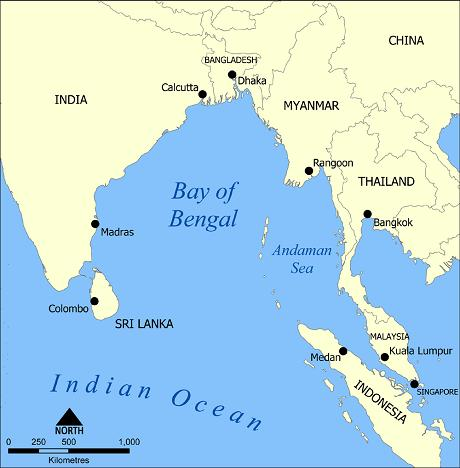
\includegraphics[width=0.5\linewidth]{CHAPTER 1/Indian Ocean Region and Key Maritime Links.png}
    \caption{Indian Ocean Region and Key Maritime Links \cite{cesak2016andaman}}
    \label{fig:placeholder}
\end{figure}
\vspace{\baselineskip}\par\noindent Beyond domestic concerns, India's strategic position straddles the world’s primary maritime Sea Lines of Communication (SLOCs). The global maritime economy depends on three critical choke points bordering the IOR: the Strait of Hormuz (facilitating the transit of Middle Eastern hydrocarbons), Bab-el-Mandeb (connecting the Red Sea to the Mediterranean via the Suez Canal) and the Strait of Malacca (the gateway to the South China Sea and the Pacific Ocean). Approximately 70\% of the global oil trade and 50\% of the world's container traffic traverse these waters annually. Consequently, any disruption to these lines, whether by state sponsored blockades, asymmetric piracy, or localized conflict, poses a direct threat to India’s economic stability and regional energy security.
\section{Fleet Capabilities and Gaps}The Indian Navy operates to project power, ensure sea control, and maintain Maritime Domain Awareness (MDA) throughout the IOR.
\subsection{Core Strengths}
\begin{enumerate}[\alph*)]
    \item \textbf{Carrier Aviation and Blue-Water Projection:}The Indian Navy is  one of a select few global forces operating multiple active Carrier Strike Groups (CSGs). The operational deployment of INS Vikramaditya and the indigenous INS Vikrant gives the navy a distinct advantage in projecting organic air power, enforcing wide-area sea control, and providing comprehensive air defense shields far beyond the range of land based aircraft.
    \begin{figure}[htbp]
        \centering
        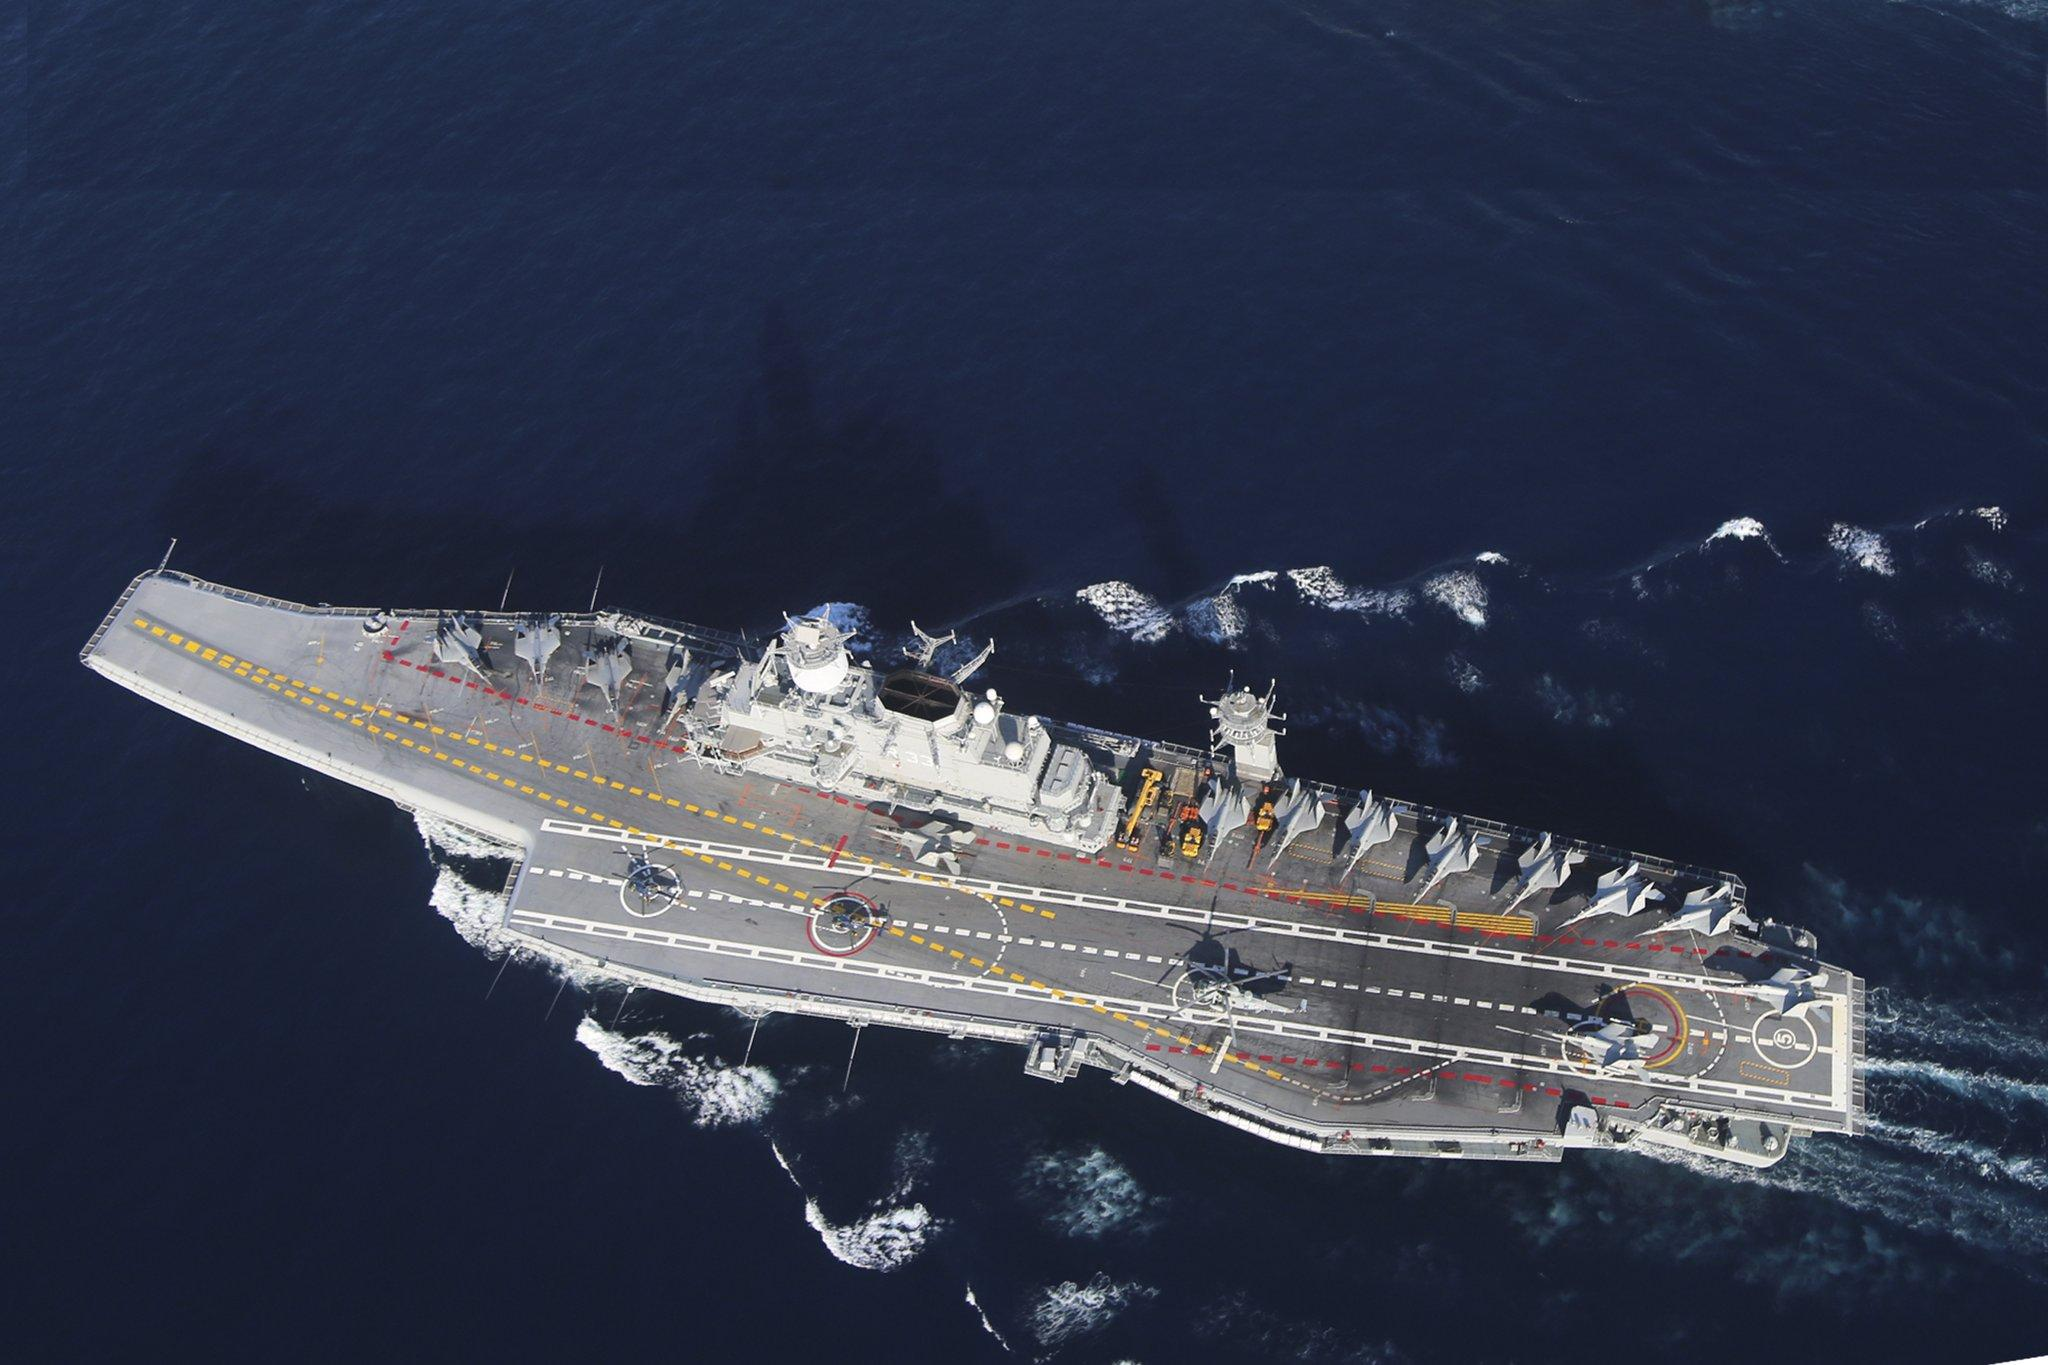
\includegraphics[width=0.75\linewidth]{CHAPTER 1/INS Vikramaditya aircraft carrier at sea.png}
        \caption{INS Vikramaditya aircraft carrier at sea \cite{indiannavy2021vikramaditya}}
        \label{fig:placeholder}
    \end{figure}
    \item \textbf{Stealth Platform Development:}Indian design capabilities have progressed through projects like the Kolkata and Visakhapatnam-class (Project 15A\&B) guided missile destroyers and the Shivalik and Nilgiri-class (Project 17\&17A) stealth frigates. These ships show advanced mastery of radar cross-section (RCS) reduction techniques, infrared signature suppression, and network-centric warfare through integrated Combat Management Systems (CMS).
    \item \textbf{Material and Technological Infrastructure: }Collaborations between the Defence Research and Development Organisation (DRDO) and the Steel Authority of India Limited (SAIL) led to the domestic production of DMR 249A and DMR 249B high-tensile warship-grade steel. This development eliminated reliance on foreign suppliers for structural hull plates.
    \begin{figure}[htbp]
        \centering
        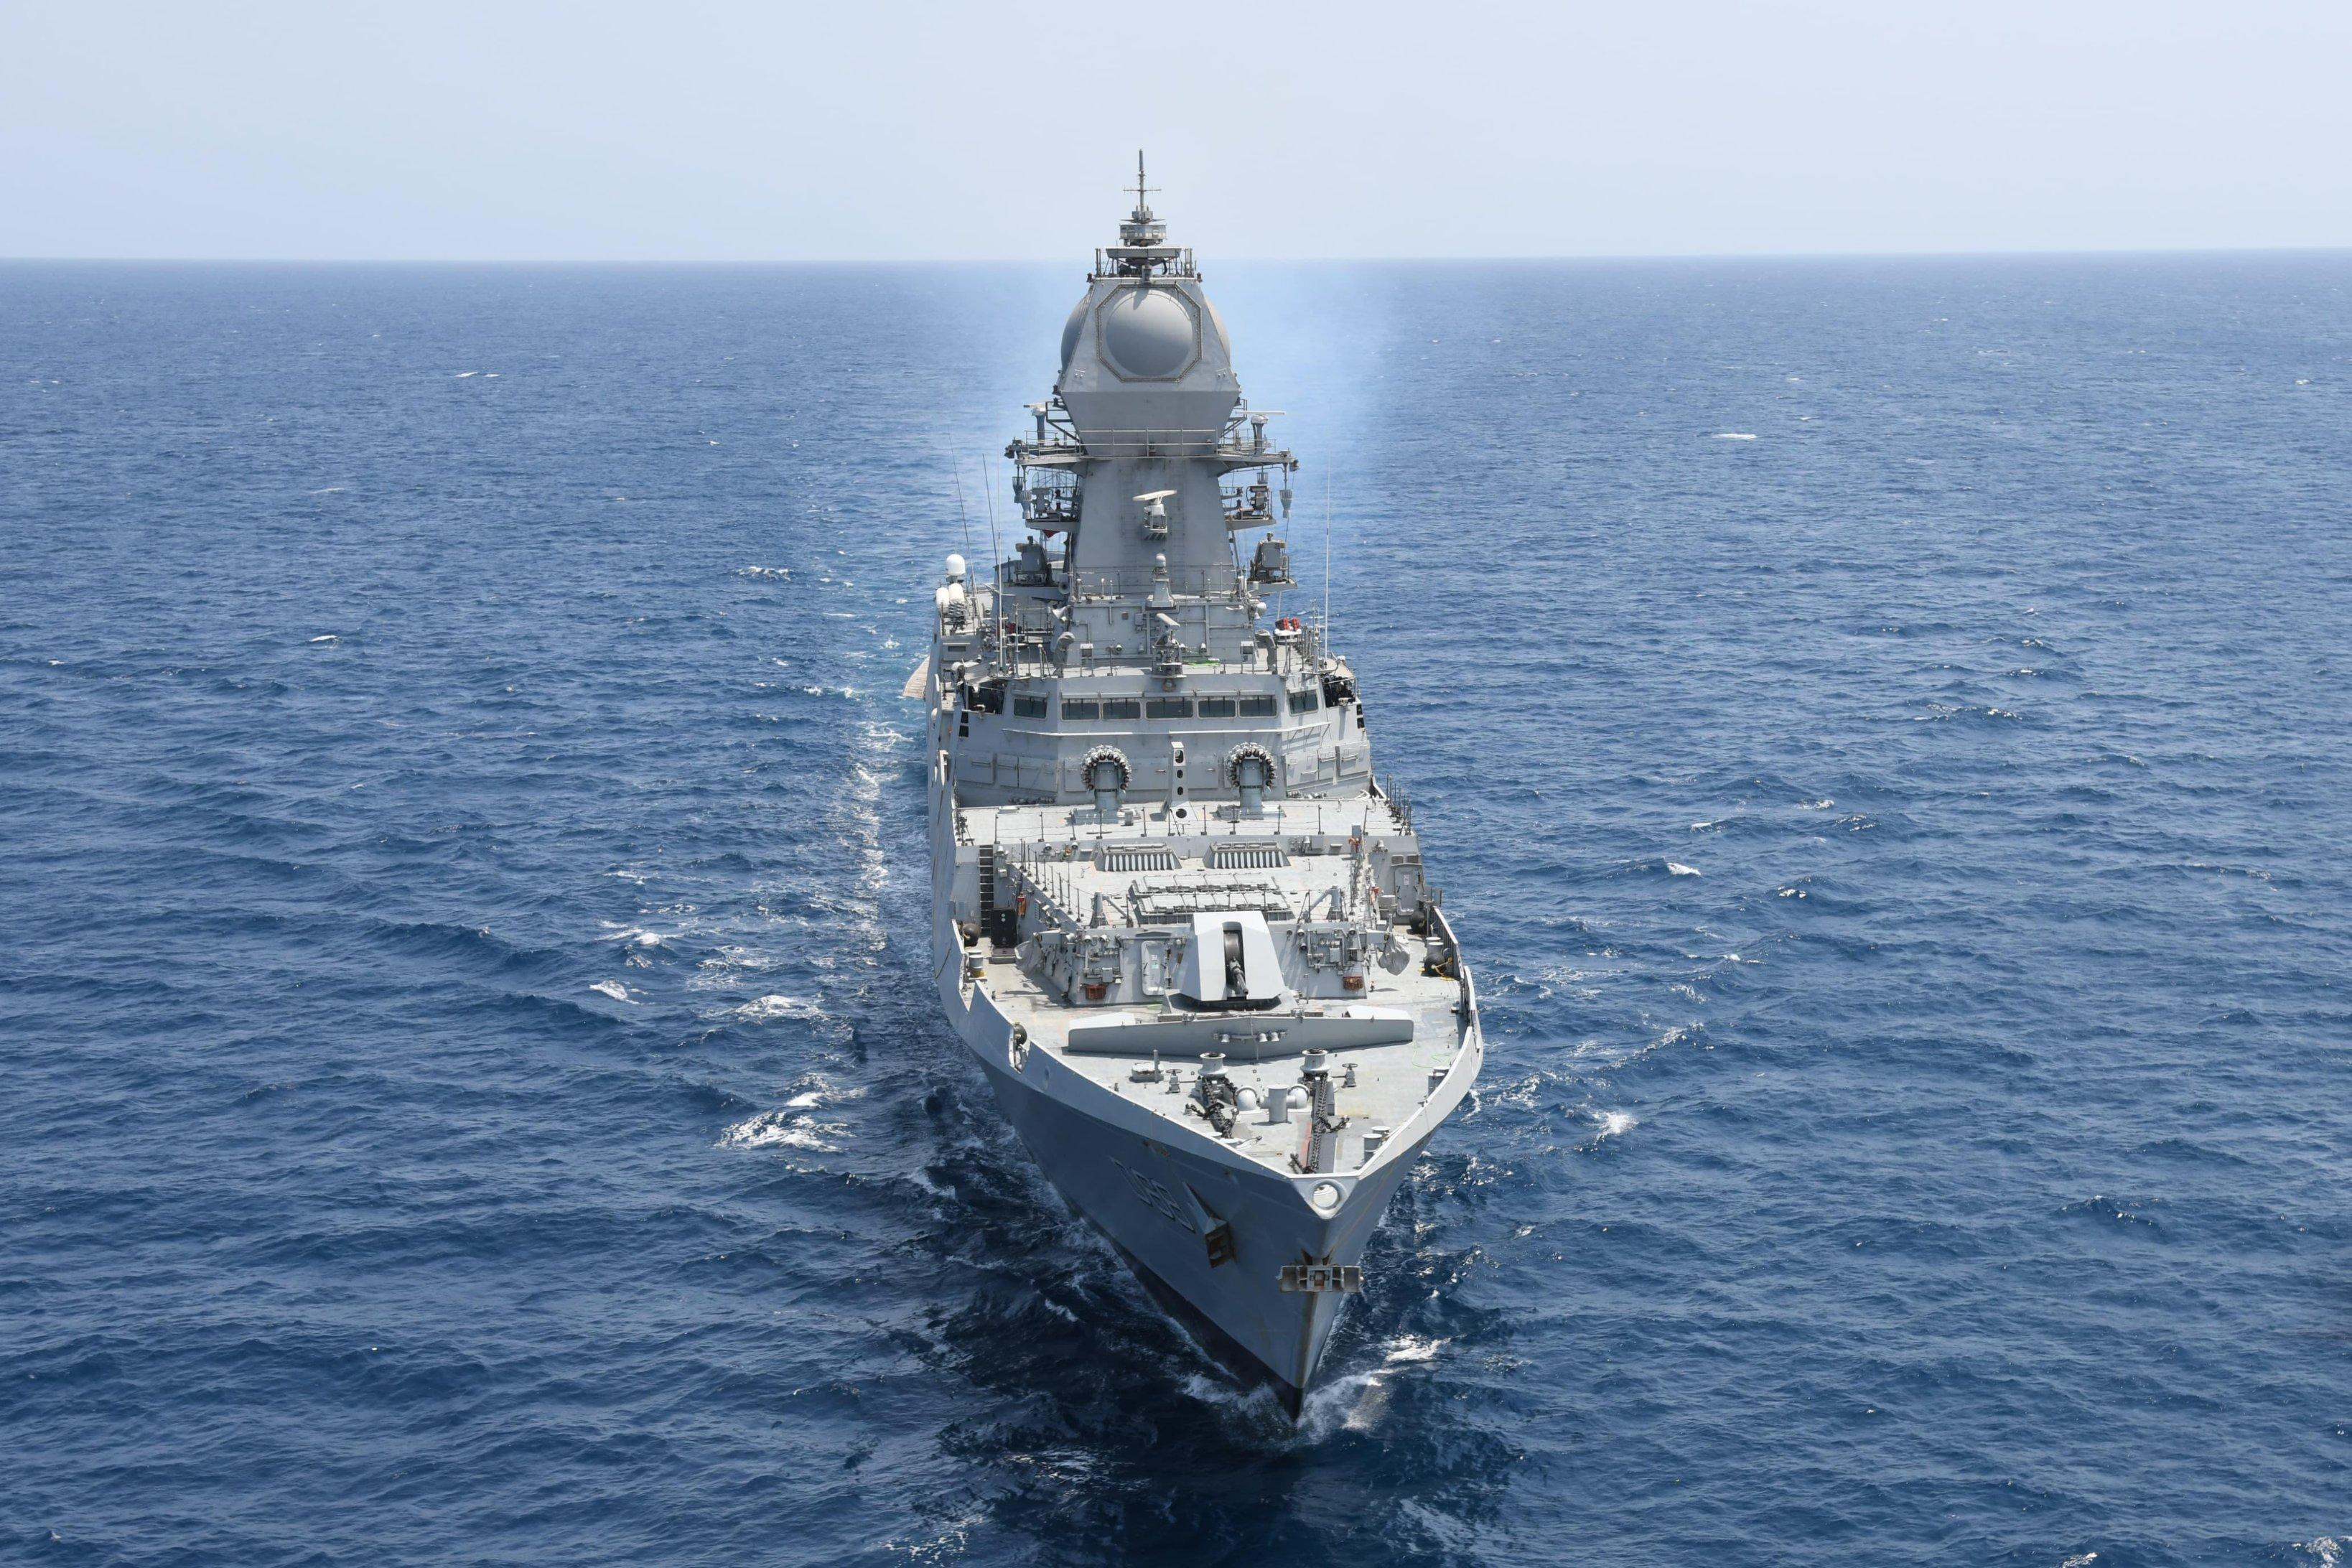
\includegraphics[width=0.75\linewidth]{CHAPTER 1/INS Imphal Project 15B destroyer.png}
        \caption{INS Imphal Project 15B destroyer \cite{indiannavy2024imphal}}
        \label{fig:placeholder}
    \end{figure}
    \item \textbf{Fiscal and Operational Inter-operability: }Decades of executing 
 highly integrated bilateral and multilateral exercises (such as Malabar and Milan) have optimized tactical communication links and cross deck helicopter logistics, positioning the Indian Navy as a primary security 
provider in the region.
\begin{table}[htbp]
    \centering
    \caption{Core Strengths and Structural Vulnerabilities}
    \label{tab:core_strengths_vulnerabilities}
    \renewcommand{\arraystretch}{1.25}
    \setlength{\tabcolsep}{8pt}
    \begin{tabular}{clcl}
        \toprule
        \multicolumn{2}{c}{\textbf{Core Strengths}} &
        \multicolumn{2}{c}{\textbf{Structural Vulnerabilities}} \\
        \midrule
        \textbf{No.} & \textbf{Description} &
        \textbf{No.} & \textbf{Description} \\
        \midrule
        1 & Carrier strike group capability &
        1 & Fleet depletion in littoral hulls \\
        
        2 & Advanced domestic stealth tech &
        2 & Critical submarine shortages \\
        
        3 & Indigenous DMR 249A steel production &
        3 & High operational asset fatigue \\
        
        4 & High inter operability standards &
        4 & Deficit in mine counter measures \\
        \bottomrule
    \end{tabular}
\end{table}


\end{enumerate}
\subsection{Structural Vulnerabilities}
\begin{enumerate}[\alph*)]
    \item \textbf{Asset Distribution Overstretch: }A critical gap exists between heavy blue-water combatants (destroyers and frigates) and light coastal assets. Using a 7,000-tonne stealth destroyer for routine anti-piracy operations, maritime border enforcement, or escort duties causes unnecessary wear and tear on complex machinery and expends disproportionate amounts of fuel.
    \item \textbf{Under-sea Warfare Shortages:}
    The conventional diesel-electric submarine fleet faces block obsolescence. Delays in procurement frameworks have caused a dip in the minimum required hull count, limiting the navy's ability to maintain continuous underwater surveillance at key maritime choke points.
    \item \textbf{Mine Counter-Measures (MCM) Shortfall: }The fleet has a noticeable deficit in dedicated Mine Counter Measure Vessels (MCMVs). This lack of modern mine hunting sonar systems and autonomous underwater vehicles (AUVs) leaves vital commercial ports and naval bases vulnerable to asymmetric naval mining.
    \begin{figure}[htbp]
        \centering
        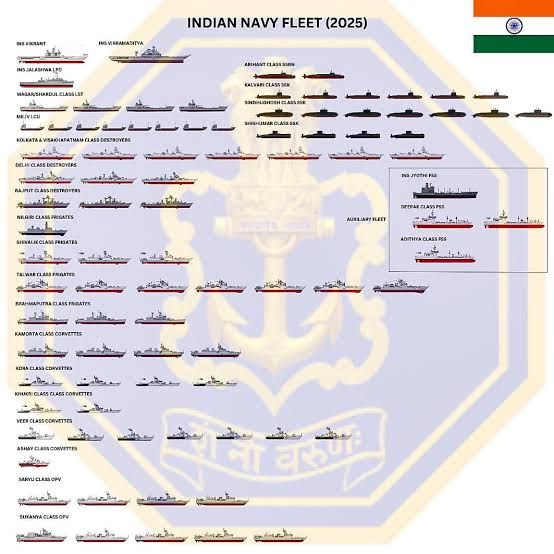
\includegraphics[width=0.75\linewidth]{CHAPTER 1/Indian Navy active fleet composition chart.jpg}
        \caption{Indian Navy active fleet composition chart}
        \label{fig:Indian Navy active fleet composition chart}
    \end{figure}
    \item \textbf{Littoral Defense Gaps: }
    Legacy missile boats (such as the Veer class) and older corvettes (like the Kora and Khukri class) lack advanced anti-submarine sonar suites, vertical launch surface-to-air missile systems, and modern stealth geometries. This leaves them vulnerable in highly contested, modern anti-access/area-denial (A2/AD) environments.
    
\end{enumerate}
\section{Threat Matrix and Security Challenges}India’s maritime operating environment is shaped by traditional state rivalries and evolving asymmetric threats. The northern Indian Ocean is increasingly contested, requiring a highly adaptable surface fleet.
\subsection{Traditional State Threats}
\label{subsec:traditional_state_threats}
\begin{figure}[htbp]
    \centering
    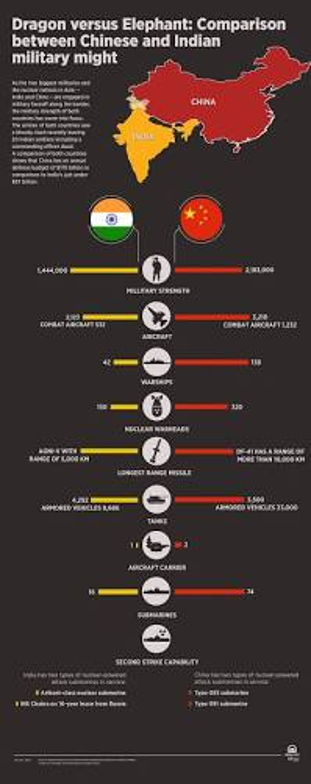
\includegraphics[width=0.3\linewidth]{CHAPTER 2/India-China military and naval strength comparison infographic.png}
    \caption{India-China military and naval strength comparison infographic}
    \label{fig:India-China military and naval strength comparison infographic}
\end{figure}

\noindent
\begin{enumerate}[\alph*)]
    \item \textbf{People's Liberation Army Navy (PLAN) Expansion:}
The Chinese Navy has expanded its presence in the IOR through its ``String of Pearls''
strategy. This involves establishing dual use commercial and military port facilities
in Gwadar (Pakistan), Hambantota (Sri Lanka), and Djibouti on the Horn of Africa.
PLAN deployments include nuclear powered attack submarines (SSNs), conventional
hunter killer submarines (SSKs), satellite-tracking ships, and hydrographic research
vessels. These assets operate inside India's maritime zone to monitor naval activities
that affect acoustic detection.
\begin{figure}[htbp]
    \centering
    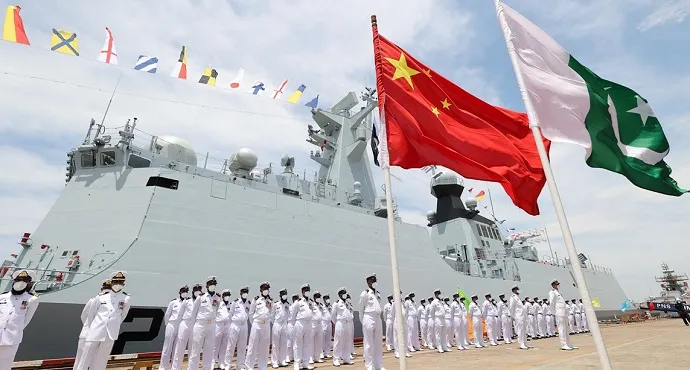
\includegraphics[width=0.75\linewidth]{CHAPTER 1/China and Pakistan “Sea Guardian” bilateral naval exercise.png}
    \caption{China and Pakistan “Sea Guardian” bilateral naval exercise \cite{iria2023seaguardian}}
    \label{fig:placeholder}
\end{figure}

\item \textbf{Pakistan Navy Modernization:}
Operating along India's western flank, the Pakistan Navy has focused on building a
specialized underwater denial force. The acquisition of advanced
\textit{Hangor} class conventional submarines equipped with Air Independent
Propulsion (AIP) allows these vessels to remain submerged for extended periods.
This presents a major challenge to surface forces in the shallow, noisy
hydroacoustic environments of the Arabian Sea.

\end{enumerate}
\subsection{Asymmetric Security Threats}
\begin{enumerate}[\alph*)]
    \item \textbf{Anti-Ship Cruise Missile (ASCM) Proliferation: }
    Low cost, high speed anti-ship missiles have spread to non state actors and proxy forces. Incidents involving sea-skimming missiles like the C-802 or variants in restricted waters like the Red Sea prove that even minor actors can threaten unstealthy surface combatants.
    \item \textbf{Unmanned Systems and Drone Swarms: }The widespread use of low-cost loitering munitions and explosive Unmanned Surface Vessels (USVs) has altered littoral warfare. A modern warship must be able to detect, track, and destroy multiple small, fast-moving surface and aerial targets simultaneously.
    \item\textbf{Transnational Maritime Crime:}The IOR continues to deal with traditional security issues, including piracy originating from the Somali basin, maritime narcotics trafficking, weapons smuggling used to fund regional insurgencies, and widespread Illegal, Unreported, and Unregulated (IUU) fishing that depletes local marine resources.
    \begin{figure}[htbp]
        \centering
        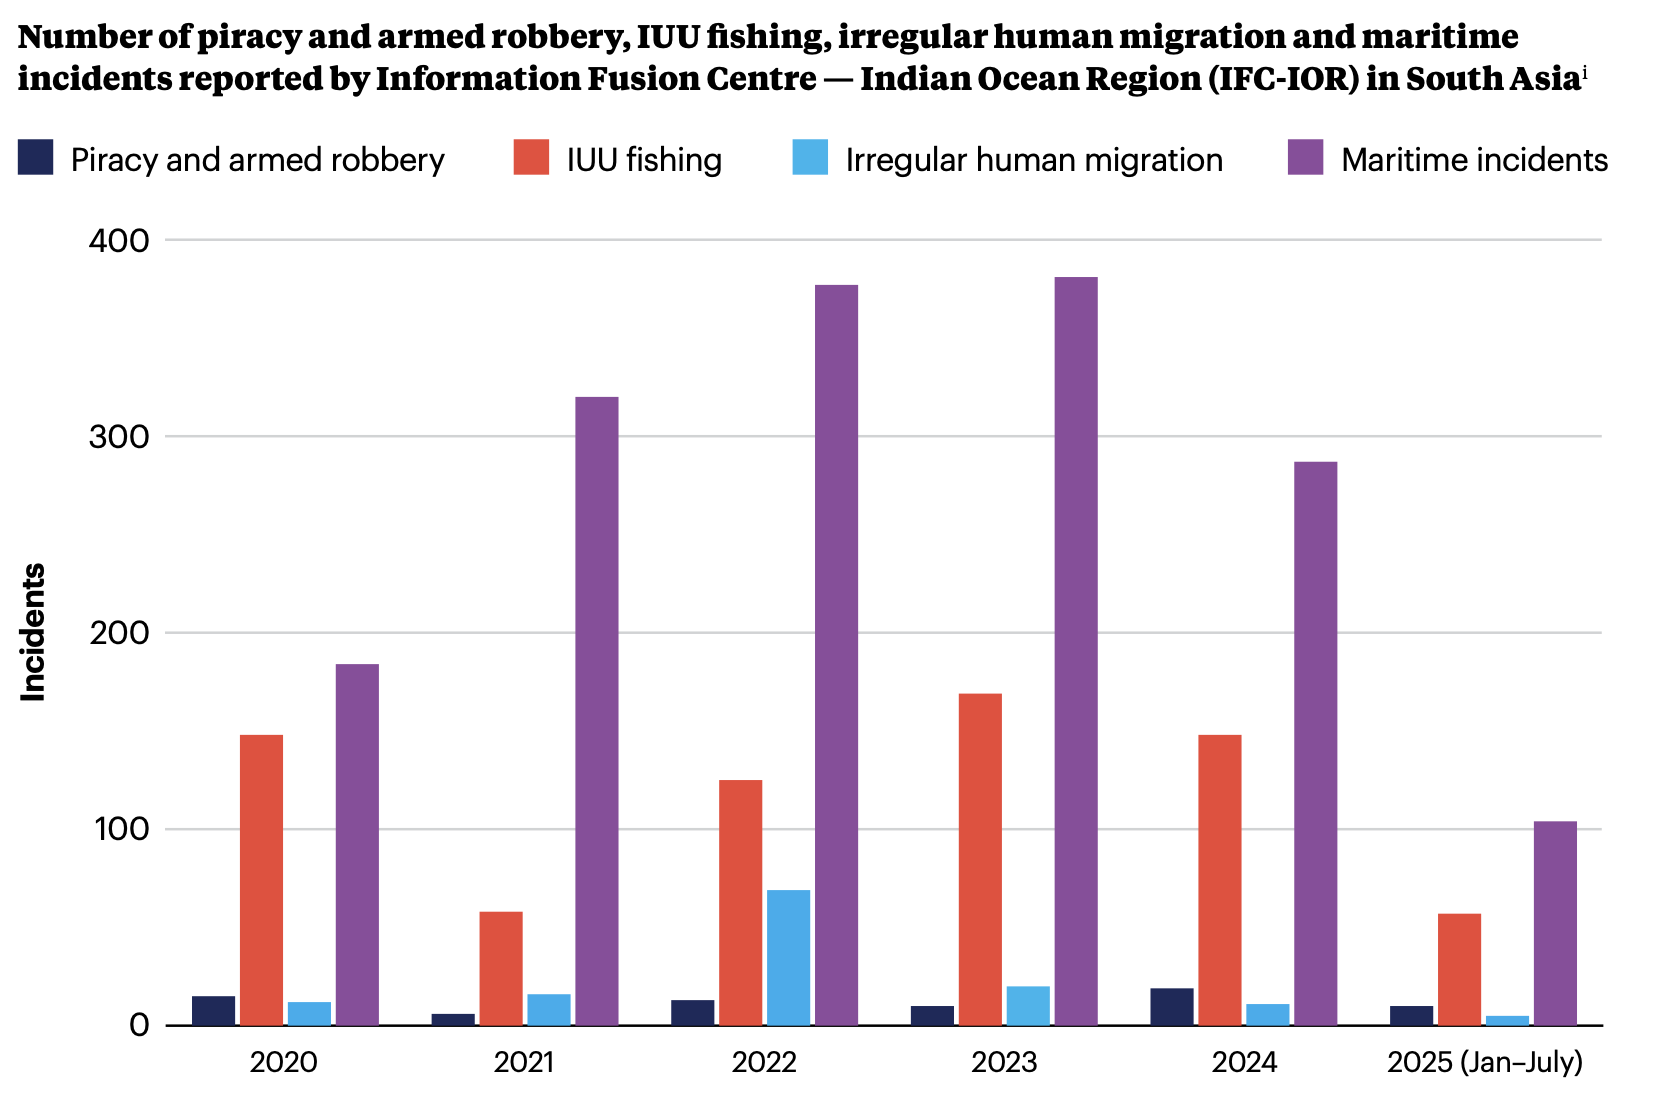
\includegraphics[width=0.75\linewidth]{CHAPTER 1/indian Ocean maritime security and crime incident graph.png}
        \caption{Indian Ocean maritime security and crime incident graph \cite{globalmaritimehub2026indianocean}}
        \label{fig:placeholder}
    \end{figure}
\end{enumerate}
\section{Technical and Tactical Role}
In naval engineering terminology, a Corvette is defined as a surface combatant falling between an Offshore Patrol Vessel (OPV) and a Frigate. It typically features a displacement of 1,000 to 3,500 tons, an overall length between 80 and 120 meters, and a hull optimized for speed, maneuverability, and shallow-drift operations.
The engineering and operational necessity of the corvette class stems from basic naval economics and hydrodynamic principles.
\subsection{Littoral Hydrodynamics and Tactical Maneuverability}
Large surface vessels such as destroyers require significant operational drafts (often exceeding 6.5 meters), making them poorly suited for shallow coastal archipelagos, sandbanks, and restricted littoral channels. The shallow draft of a corvette (typically less than 4.5 meters) allows it to navigate these confined spaces easily. This shallow draft provides access to smaller ports and offers tactical cover near irregular coastlines, where land clutter can disrupt enemy radar tracking.
\subsection{The Weapon to Displacement Efficiency Ratio}
Modern structural design, lightweight composite superstructures, and compact weapon electronics allow engineers to mount heavy armament onto smaller hulls. A modern 3,500-ton corvette can carry supersonic anti-ship cruise missiles, active towed array sonars, torpedo launchers, and vertical launch air defense networks capabilities previously restricted to 6,000-ton frigates.
\subsection{Operational Cost Optimization}
Building and maintaining a destroyer requires significant capital expenditure and large crew complements (often more than 250 personnel). In contrast, a corvette integrates extensive automation such as automated machinery control systems (AMCS) and smart damage control systems which reduces the crew's requirements to fewer than 150 personnel. This lower manning requirement, combined with a smaller displacement, reduces fuel consumption and lowers overall lifecycle costs while keeping a highly capable combat asset at sea.
\section{Evolution of Fleet Hulls}
The development of the Indian Navy's corvette fleet marks a clear transition from basic foreign imports to advanced, domestically designed stealth platforms.
\subsection{Legacy Strike Hulls}
The older framework relied on Veer class missile boats (derived from the Soviet Project 1241RE Tarantul class) and Kora class guided-missile corvettes. These platforms offered high speeds and heavy forward fire networks, but lacked comprehensive multi-mission capabilities, offering limited air defense and minimal anti-submarine protection.
\subsection{Project 28 (Kamorta Class)}
To address the growing threat of submarines in the region, the Directorate of Naval Design developed the Project 28 Kamorta-class ASW corvette. Built by Garden Reach Shipbuilders \& Engineers (GRSE) in Kolkata, these vessels have a full load displacement of 3,300 to 3,500 tons, an overall length of 109.1 meters and a beam of 13.7 meters.
\vspace{\baselineskip}\par\noindent The Project 28 class introduced several key structural innovations:
\begin{enumerate}[\alph*)]
    \item \textbf{Advanced Stealth Geometries: }The hull utilizes an 'X-form' cross section with inclined superstructure bulkheads to scatter incoming radar waves, significantly lowering the vessel's radar cross-section.
    \begin{figure}[htbp]
        \centering
        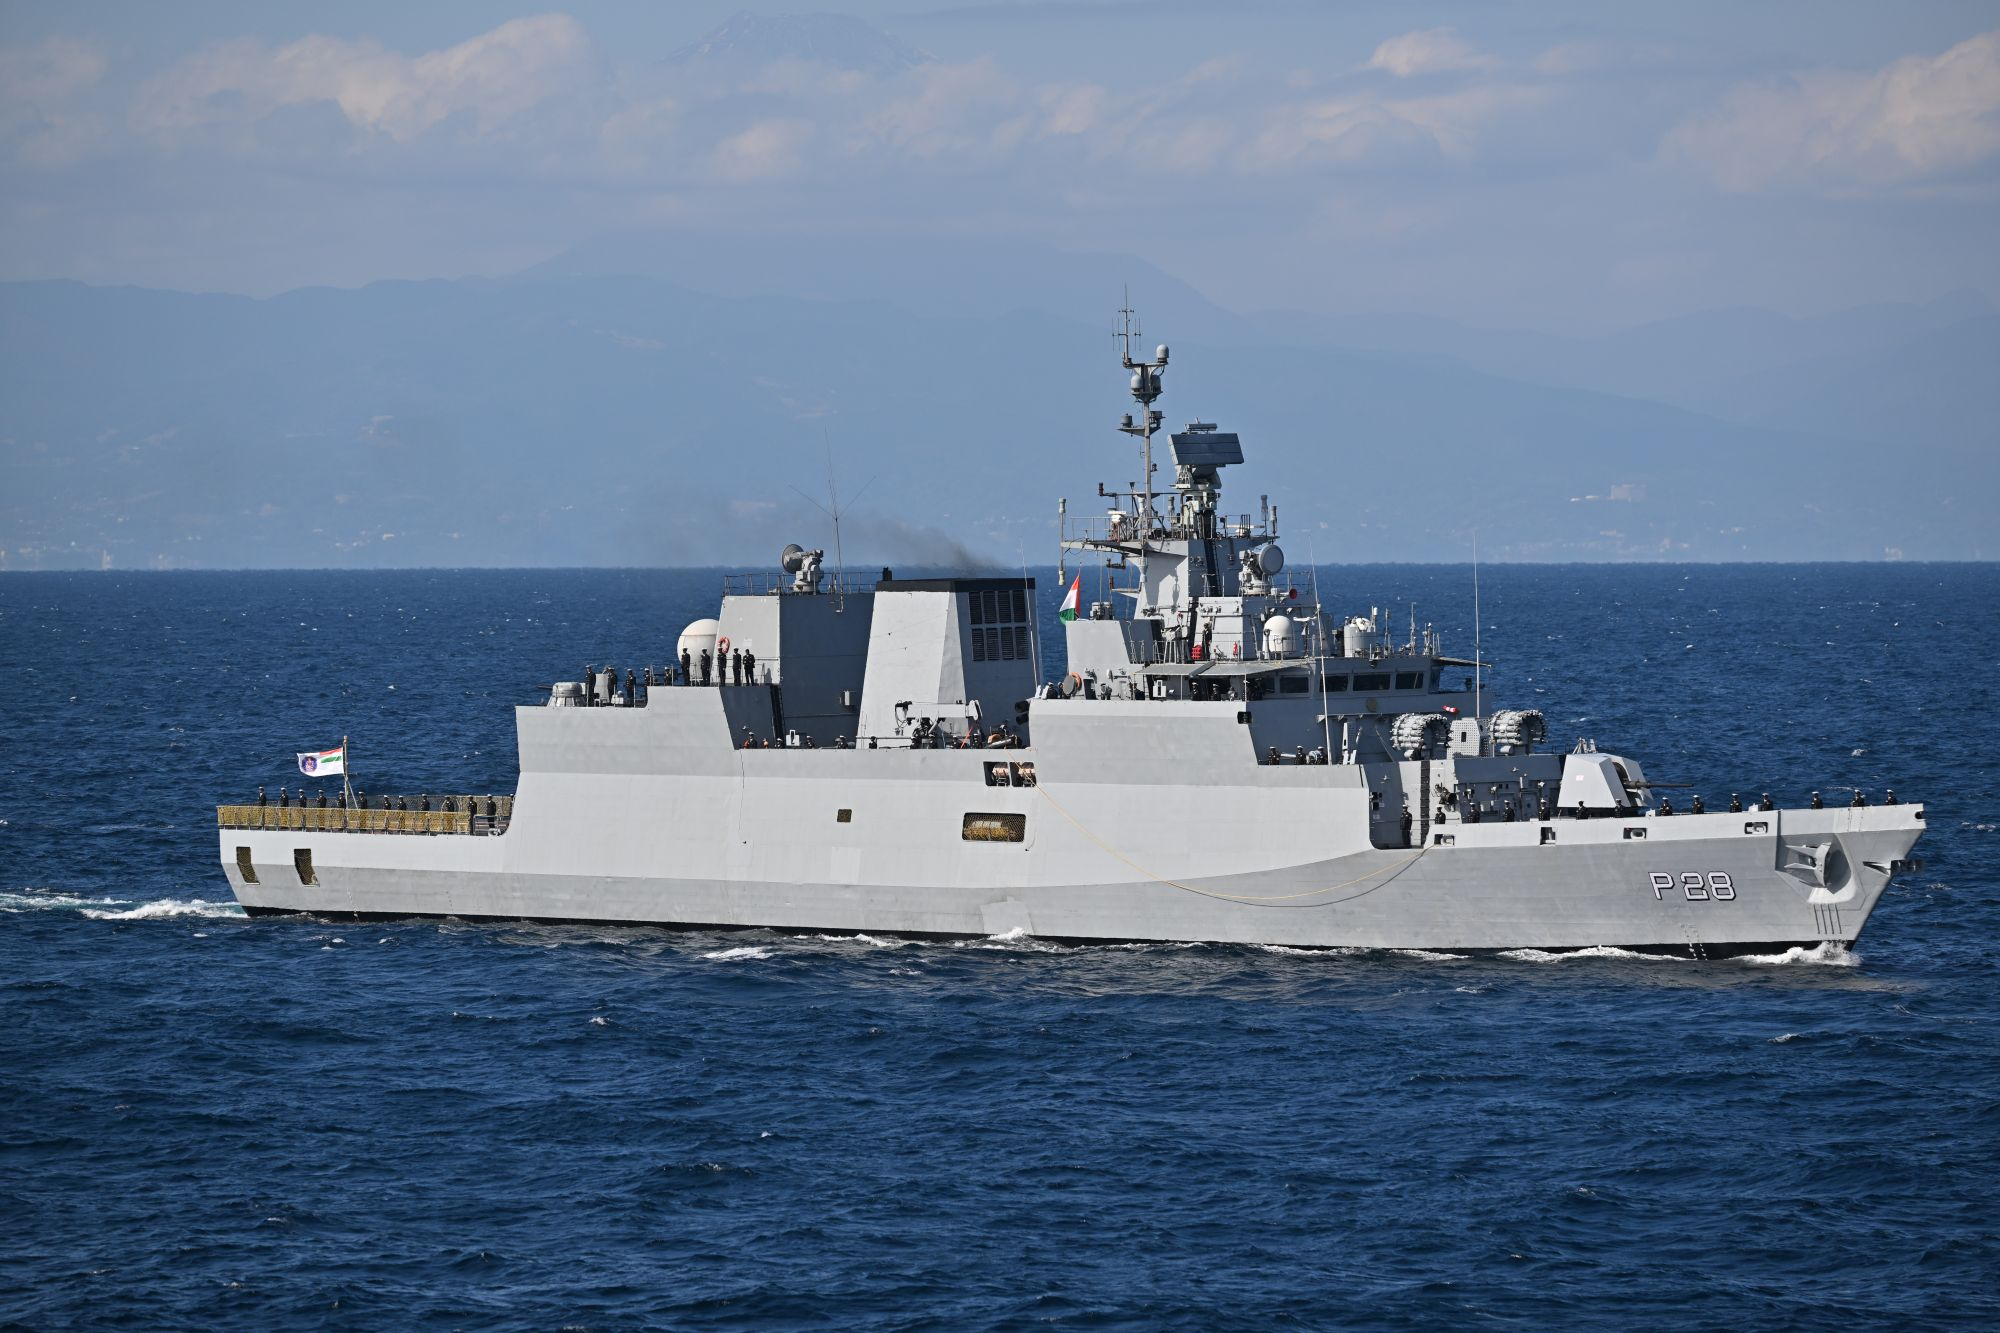
\includegraphics[width=0.7\linewidth]{CHAPTER 1/INS Kamorta antisubmarine corvette at sea.png}
        \caption{INS Kamorta antisubmarine corvette at sea \cite{bharatpedia2026kamorta}}
        \label{fig:placeholder}
    \end{figure}
    \item \textbf{Composite Superstructure Integration: }The upper superstructure incorporates Carbon Fiber Reinforced Plastic (CFRP) structural panels co-bonded to the steel hull structure. This lowered the ship’s vertical center of gravity, which improved intact stability margins and reduced overall structural weight.
    \item \textbf{Acoustic Quieting and Vibration Isolation: }
    The main machinery is mounted on specialized raft isolation systems. This arrangement absorbs structural vibrations before they reach the hull plating, reducing the underwater radiated noise signature to hamper detection by enemy passive sonars.
    \item \textbf{Propulsion System: }
    The propulsion plant uses a Combined Diesel and Diesel (CODAD) configuration, pairing four Pielstick 12 PA6 STC diesel engines to drive twin controllable-pitch propellers, achieving a top speed of 32 knots and an economical cruising range of 4,000 nautical miles at 14 knots.
\end{enumerate}
\section{Next Gneration Missile Vessels (NGMV)}
Designed to replace the aging Veer class, the NGMV is a specialized anti-surface strike vessel. Displacing roughly 1,437 tons with an overall length of 89 meters and a narrow beam of 12 meters, these ships are engineered for high-speed dashes.
\vspace{\baselineskip
}\par\noindent The propulsion layout uses a Combined Diesel and Gas (CODAG) system that pairs a General Electric LM2500 gas turbine with two cruising diesel engines to power three Kongsberg Kamewa waterjets. This setup enables a maximum speed of 35 knots. The primary armament consists of eight BrahMos supersonic anti-ship cruise missiles carried in slant-launch configurations, combined with a 24 cell Vertical Launch Short Range Surface-to-Air Missile (VL-SRSAM) system for point defense.
\subsection{Next Generation Corvettes (NGC)}
The future core of the littoral combat fleet is the Next Generation Corvette program. Approved by the Ministry of Defense, this program involves constructing eight multi-role surface combatants, with GRSE serving as the lead shipyard for five hulls and Goa Shipyard Limited (GSL) building the remaining three.
\begin{figure}[htbp]
    \centering
    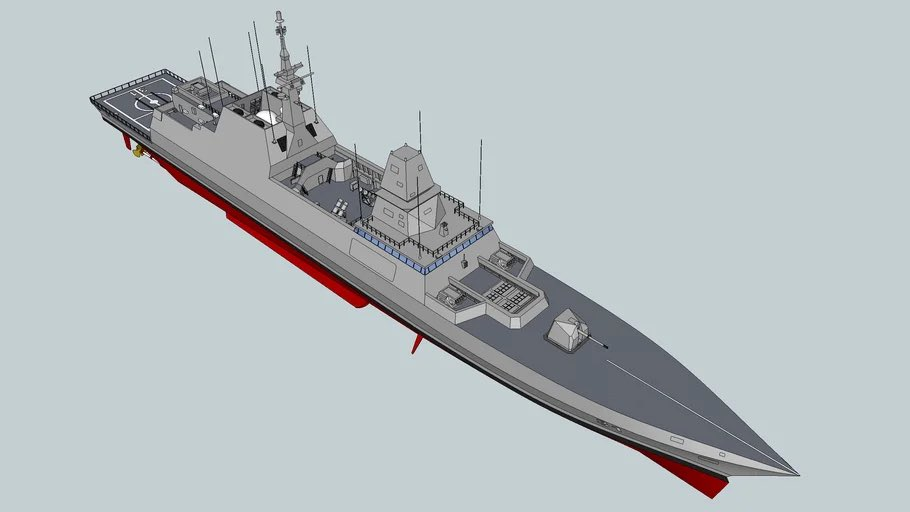
\includegraphics[width=0.8\linewidth]{CHAPTER 1/Indian Navy Next Generation Corvette (NGC) schematic concept.png}
    \caption{Indian Navy Next Generation Corvette (NGC) schematic concept \cite{defencedecode2025post}}
    \label{fig:placeholder}
\end{figure}
The NGC features a planned displacement of 3,800 to 4,000 tons, a length of under 120 meters, and a beam of under 15 meters. The propulsion system will utilize a robust CODAG network, combining two Rolls-Royce MT30 gas turbines with four indigenous 6 MW diesel engines to ensure a sustained cruising range of 4,000 nautical miles at 14 knots and top speeds exceeding 27 knots. The armament suite includes eight BrahMos cruise missiles, 24 vertical launch anti-missile defense cells, and dual triple-tube 324 mm lightweight torpedo launchers.
\section{Operational History and Case Studies}
Small, heavily armed surface vessels have played a critical role in major operations conducted by the Indian Navy, validating their operational concept through direct combat success.
\subsection{Operations Trident and Python (1971)}
During the 1971 Indo-Pakistani War, the Indian Navy deployed Osa class missile boats the technological precursors to the modern missile corvette in offensive operations. On 4 December 1971, under Operation Trident, these agile vessels executed a high speed strike against the Pakistani naval hub at Karachi.
\begin{figure}[htbp]
    \centering
    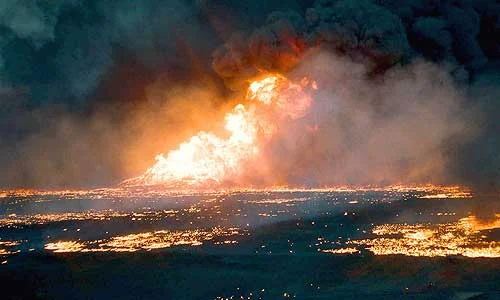
\includegraphics[width=0.75\linewidth]{CHAPTER 1/Karachi harbor burning during Operation Trident.png}
    \caption{Karachi harbor burning during Operation Trident \cite{iadn_operationtrident}}
    \label{fig:placeholder}
\end{figure}
Firing Soviet supplied P-15 Termit anti-ship missiles, they sank the destroyer PNS Khaibar and the minesweeper PNS Muhafiz, while severely damaging merchant assets and shore based fuel storage tanks. Days later, Operation Python struck the port again, crippling the local maritime logistics network. These actions established sea control for India in the northern Arabian Sea and demonstrated the striking power of small, fast missile combatants.

\subsection{Operation Vijay and Operation Talwar (1999)}
During the 1999 Kargil Conflict, the Indian Navy launched Operation Talwar to put aggressive pressure on Pakistan's maritime trade routes. Missile corvettes were deployed alongside larger destroyers to form a tight naval blockade in the northern Arabian Sea.
\vspace{\baselineskip}\par\noindent This forward deployment cut off commercial fuel routes to Karachi and discouraged the possible escalation of the Pakistani navy. The ability of corvettes to operate effectively near shallow coastal borders allowed larger capital ships to maintain broader sea-denial screens further out at sea.
\subsection{Anti-Piracy and Escort Deployments (2000s – Present)}
In response to the rise of piracy in the western Indian Ocean and the Gulf of Aden, the Indian Navy has maintained a continuous presence in these high-risk areas. Corvettes have proven highly effective for these missions. Their operational endurance allows them to conduct extended patrols, while their onboard helicopter facilities and rigid hull inflatable boats (RHIBs) enable rapid boarding actions. Deploying corvettes for these tasks keeps international sea lanes open while preserving larger destroyers for primary defense duties elsewhere.
\section{Modular Design Principles}
A fundamental aspect of modern corvette design is the adoption of modular payload architectures. Historically, warships were designed around fixed systems; weapons and sensors were permanently integrated into the structural fabric of the hull. This traditional approach meant that mid-life refits took years to complete, requiring extensive structural cutting, welding, and balance reconalibrations.
\vspace{\baselineskip}\par\noindent A fundamental aspect of modern corvette design is the adoption of modular payload architectures. Historically, warships were designed around fixed systems; weapons and sensors were permanently integrated into the structural fabric of the hull. This traditional approach meant that mid life refits took years to complete, requiring extensive structural cutting, welding, and balance reconalibrations.
Modern corvette engineering solves this issue using standardized interfaces such as standardized containerized mission slots which allow systems to be quickly swapped out.
\subsection{Structural and Utility Standardization}
Mission bays are engineered with uniform spatial dimensions, structural load foundations, standard electrical connections, and uniform cooling water systems. This design allows the vessel's primary role to be reconfigured within 48 hours at a forward naval base.
\begin{figure}[htbp]
    \centering
    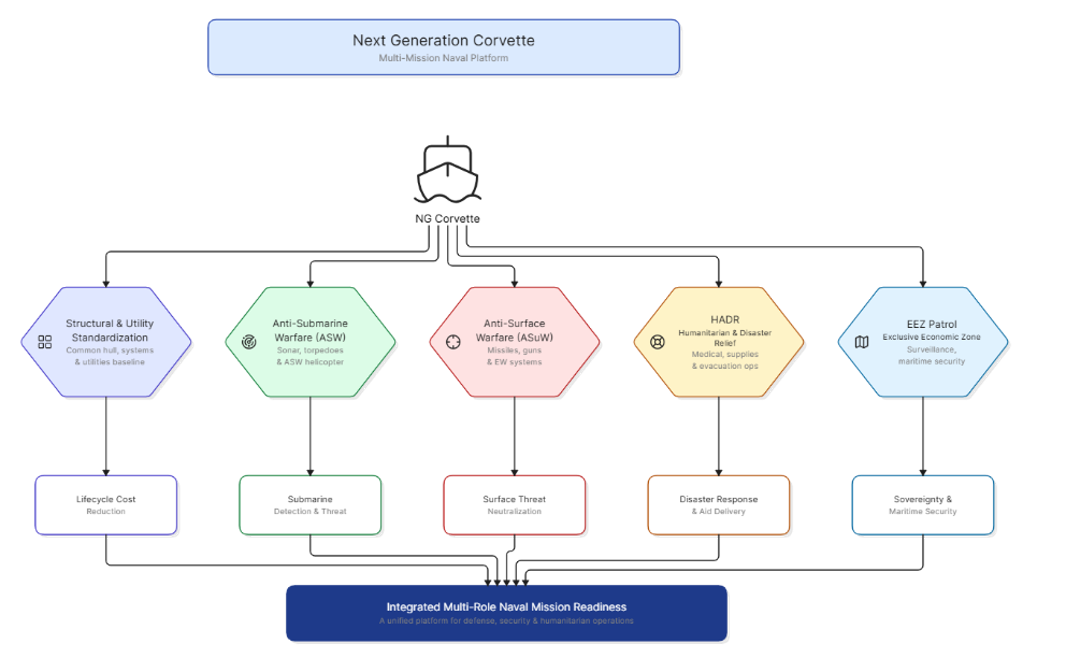
\includegraphics[width=1\linewidth]{CHAPTER 1/Concept of NGC.png}
    \caption{Concept of NGC}
    \label{fig:placeholder}
\end{figure}
\subsection{Anti-Submarine Warfare (ASW) Mode}
The modular bay is equipped with an active towed array sonar system, processing racks, and lightweight torpedo storage systems.
\subsection{Anti-Surface Warfare (ASuW) Mode}
The ASW systems are removed and replaced with containerized surface-to-surface missile launch systems or long-range loitering munitions to boost surface striking power.
\subsection{Humanitarian Assistance and Disaster Relief (HADR) Mode}
The weapons modules are replaced with mobile medical stations, water purification machinery, and emergency supplies, allowing the corvette to act as a first responder during regional environmental crises.
\section{Signature Management Systems}
Surviving in modern contested littorals requires a comprehensive approach to signature management. Because corvettes operate closer to hostile coastlines than larger frigates, they face higher exposure to land-based radar installations, thermal imaging networks, and shallow water acoustic sensor arrays.
\begin{figure}[htbp]
    \centering
    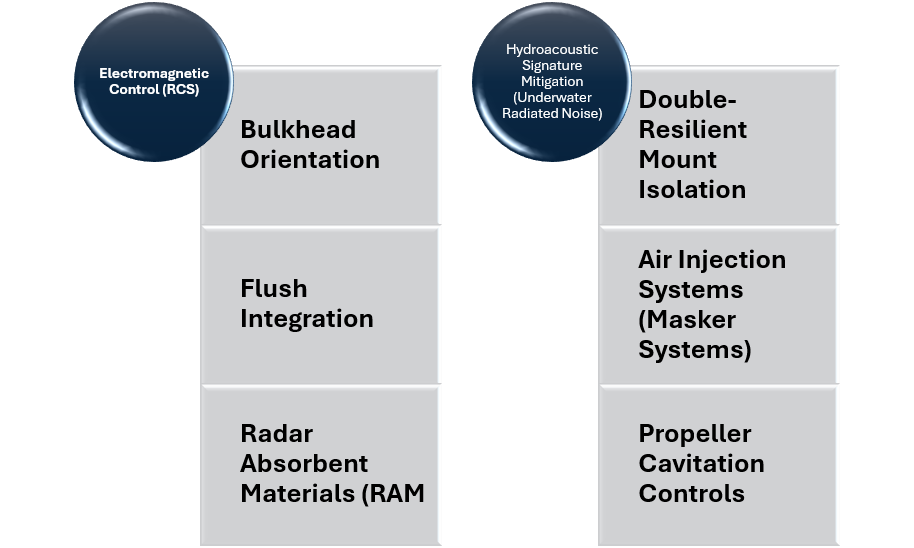
\includegraphics[width=1\linewidth]{CHAPTER 1/Signature Management System.png}
    \caption{Signature Management System}
    \label{fig:placeholder}
\end{figure}
\subsection{Electromagnetic Control (RCS)}
Reducing the vessel's Radar Cross-Section relies on geometric configuration and advanced material placement:
\begin{enumerate}[\alph*)]
    \item \textbf{Bulkhead Orientation: }
    Superstructure slopes are maintained at angle configurations between 10 degrees to 15 degrees relative to the vertical plane. This angle prevents orthogonal radar reflections, scattering incoming electromagnetic waves away from the enemy receiver antenna.
    \item \textbf{Flush Integration: }Deck equipment including mooring winches, bitts, and chocks is positioned beneath the main deck or hidden behind clean bulwark screens.
    \item \textbf{Radar Absorbent Materials (RAM): }The superstructure is treated with specialized multi-layer dielectric and magnetic RAM coatings. These coatings convert incoming electromagnetic energy into thermal energy, significantly reducing the ship's overall radar detection range.
\end{enumerate}
\subsection{Hydroacoustic Signature Mitigation (Underwater Radiated Noise)}
Passive acoustic sonars in enemy submarines represent a serious threat to the surface hulls. Minimizing Underwater Radiated Noise requires isolated machinery layouts.
\begin{enumerate}[\alph*)]
    \item \textbf{Double-Resilient Mount Isolation: }
    Main propulsion diesels and diesel generator sets are attached to an intermediate structural raft plate via elastomeric isolators. This assembly is then mounted to the ship's primary framing network using a second set of high-deflection rubber isolators, blocking structural vibrations from reaching the outer hull plating.
    \item \textbf{Air Injection Systems (Masker Systems): }
    Perforated air emitter bands are installed along the hull's exterior near the engine spaces. These bands discharge a continuous screen of micro bubbles into the boundary layer, altering the local acoustic impedance and dampening internal machinery noise.
    \item \textbf{Propeller Cavitation Controls: }
    Propeller blade geometries are optimized using advanced computational fluid dynamics (CFD) to delay the onset of tip cavitation. Additionally, air is injected through the propeller hub and out along the blade edges (Pratt Prairie systems) to collapse cavitation bubbles smoothly, reducing high-frequency acoustic emissions.
\end{enumerate}
\section{The Strategic Imperative for Indigenous Shipbuilding(Aatmanirbhar Bharat)}Transitioning from foreign procurement to absolute domestic self-reliance 
(Aatmanirbhar Bharat) is a key requirement for modern Indian warship design. 
Historically, relying on foreign shipyards created significant vulnerabilities: 

\subsection{Geopolitical Sanction Risks }
Relying on foreign suppliers leaves naval construction programs 
vulnerable to sudden changes in international relations, technology 
transfer restrictions, and unilateral sanctions. These external  
disruptions can block spare part pipelines during periods of active 
conflict.
\subsection{Lifecycle and Configuration Control}
When a warship is designed and built domestically, the navy retains 
absolute control over its configuration management data. This allows 
engineers to modify structural frames, update software code in the 
Combat Management System, and replace aging electronic subsystems 
without requiring permission or documentation from a foreign original 
equipment manufacturer (OEM).


\section{Outline Specifications}
\begin{longtable}{@{}p{0.24\textwidth}p{0.70\textwidth}@{}}
\caption{Outline Specifications of the Proposed Multi-Role Corvette}
\label{tab:outline_specifications} \\

\toprule
\textbf{Parameter} & \textbf{Specification} \\
\midrule
\endfirsthead

\toprule
\textbf{Parameter} & \textbf{Specification} \\
\midrule
\endhead

\bottomrule
\endfoot

% General Characteristics
\multicolumn{2}{@{}l}{\textbf{General Characteristics}} \\
\midrule

Type &
Multi-Role Corvette \\

Role &
Anti-Submarine Warfare, Anti-Surface Warfare, Air Defence,
Maritime Surveillance, EEZ Patrol and Mine Warfare Support \\

Displacement &
3,500--4,000 t \\

Length Overall &
112--118 m \\

Beam &
15--17 m \\

Draft &
5.0--5.5 m \\

Speed &
26--28 knots (Maximum); 20 knots (Cruising) \\

Range &
4,000--5,000 nautical miles at 20 knots \\

Endurance &
20--30 days \\

% Combat Capability
\midrule
\multicolumn{2}{@{}l}{\textbf{Combat Capability}} \\
\midrule

Primary Mission &
Multi-Role \\

Secondary Missions &
Maritime Security, Coastal Defence, Convoy Escort,
Search \& Rescue, Humanitarian Assistance and Disaster Relief \\

Operational Capability &
Anti-Submarine Warfare, Anti-Surface Warfare,
Local Area Air Defence and Mine Warfare Support \\

Mission Flexibility &
Modular payloads and future mission upgrades \\

% Aviation Facilities
\midrule
\multicolumn{2}{@{}l}{\textbf{Aviation Facilities}} \\
\midrule

Flight Deck &
Capable of operating one medium naval helicopter \\

Hangar &
Enclosed hangar for one helicopter and UAV facilities \\

% Mission Systems
\midrule
\multicolumn{2}{@{}l}{\textbf{Mission Systems}} \\
\midrule

Mission Bay &
Multi-purpose mission space for modular equipment \\

Unmanned Systems &
Provision for UAV, USV and AUV operations \\

Boat Facilities &
RHIB launch and recovery arrangement \\

% Accommodation
\midrule
\multicolumn{2}{@{}l}{\textbf{Accommodation}} \\
\midrule

Crew &
70--90 personnel \\

Mission Personnel &
20--35 specialists \\

Medical Facilities &
Sickbay, isolation room and first aid facility \\

% Propulsion
\midrule
\multicolumn{2}{@{}l}{\textbf{Propulsion}} \\
\midrule

Type &
CODAD \\

Propulsion &
Twin-shaft configuration \\

Bow Thrusters &
If required \\

Power Generation &
Diesel Gen Sets \\

% Self Defence
\midrule
\multicolumn{2}{@{}l}{\textbf{Self Defence and Survivability}} \\
\midrule

Weapons &
Medium Calibre Naval Gun, Close-In Weapon System (CIWS),
Surface-to-Air Missiles, Anti-Ship Missiles and Lightweight Torpedoes \\

Electronic Systems &
ESM Suite, Decoy Launchers, Electronic Countermeasures
and Electro-Optical Fire Control \\

% Design Considerations
\midrule
\multicolumn{2}{@{}l}{\textbf{Design Considerations}} \\
\midrule

Standards &
Naval Classification Rules and Naval Ship Code \\

Stealth Design &
Reduced Radar Cross Section, Infrared Signature Reduction
and Low Acoustic Signature \\

Modular Design &
Reserved Space, Weight and Power Margins for future weapons
and sensors \\

Automation &
High Platform Automation with Reduced Crew Requirements \\

Redundancy &
Enhanced System Redundancy \\

Sea Keeping &
Optimized for sustained operations in littoral and open-sea
conditions up to Sea State 6 \\

\end{longtable}



\begin{figure}[htbp]
    \centering

    \begin{minipage}{0.3\textwidth}
        \centering
        
\includegraphics[width=\linewidth]{CHAPTER 1/QR CODE.png}
    \end{minipage}
    \hfill
    \begin{minipage}{0.68\textwidth}
        \raggedright
        \textit{Scan the QR code to access the digital copy of this chapter,
        together with the LaTeX code, Excel calculations and reference bib.tex}.
    \end{minipage}

\end{figure}
\clearpage
\thispagestyle{empty}
\null
\newpage


%----------------------CHAPTER 2 BEGINS---------------------------------------------
%---------------- CHAPTER DIVIDER PAGE ----------------
\clearpage
\thispagestyle{empty}

\begin{center}
    \vspace*{\fill}

    {\fontsize{16}{19}\selectfont\bfseries CHAPTER 2\par}
    \vspace{0.6cm}
    {\fontsize{16}{19}\selectfont\bfseries FIXING OF MAIN DIMENSIONS\par}

    \vspace*{\fill}
\end{center}

\clearpage
%-------------------------------------------------------
\clearpage
\thispagestyle{empty}
\null
\newpage
    \chapter{Fixing of Main Dimensions}
    \section{Introduction}
    Designing a warship is an exercise in balancing the requirements of the ship with its physical dimensions. Before any structural lines can be drawn or internal layouts finalized, we must answer a core question: What are the physical dimensions required for this ship to successfully perform its intended missions?
    \subsection{The Influence of Dimensions on Vessel Performance}
    The dimensions of a warship dictate its operational effectiveness, crew comfort, and survival in harsh sea states.
\begin{enumerate}[\alph*)]
    \item\textbf{Seakeeping and Crew Comfort:}The length-to-beam (L/B) and beam-to-draft (B/T) ratios heavily influence the ship’s motion in heavy seas. A hull that is too short or overly wide will experience harsh, rapid roll periods, leading to severe crew fatigue and making precision tasks—such as helicopter operations on the flight deck—extremely hazardous.
    \item \textbf{Hydrodynamic Resistance:}	The slenderness ratio  ${L/\nabla^{1/3}}$ determines how efficiently the hull cuts through water. A longer, sleeker hull reduces wave-making resistance at high speeds, allowing the vessel to reach its tactical sprint targets without requiring an excessively large, heavy engine plant.
    \item \textbf{	Internal Space and Volumetric Layout:}The beam and depth control the total enclosed volume available for machinery, weapons, ammunition storage, fuel bunkers, and living quarters.
    \end{enumerate}
    \subsection{Why Parent Ship Analysis Fails for Corvettes}In commercial naval architecture—such as the design of bulk carriers, tankers, or container vessels—main dimensions are typically fixed using Parent Ship Analysis. This method relies on scaling a new design from an existing, successful "parent" vessel using linear scaling factors and empirical statistical regressions.
    \vspace{\baselineskip}\par\noindent Although parent ship analysis works well for commercial ships (which are primarily driven by volume or dead weight and share uniform hull geometries), it is fundamentally inaccurate for modern corvettes \vspace{\baselineskip} \par\noindent Warships are fundamentally weight- and payload-driven platforms, both approaches are depicted in Figure \ref{fig:my_label}. Two corvettes of identical length can have completely different internal requirements. For example, a specialized Anti-Submarine Warfare (ASW) corvette that requires heavy sonar arrays, acoustic insulation, and helicopter hangar facilities demands an entirely different volumetric footprint than an Anti-Surface missile craft (ASuW) dominated by heavy vertical launch systems (VLS). Applying simple scaling factors from a parentship risks either under-sizing critical combat spaces or over-sizing the hull, which unnecessarily increases build costs and radar signatures.

\vspace{\baselineskip}
    \begin{figure}
        \centering
        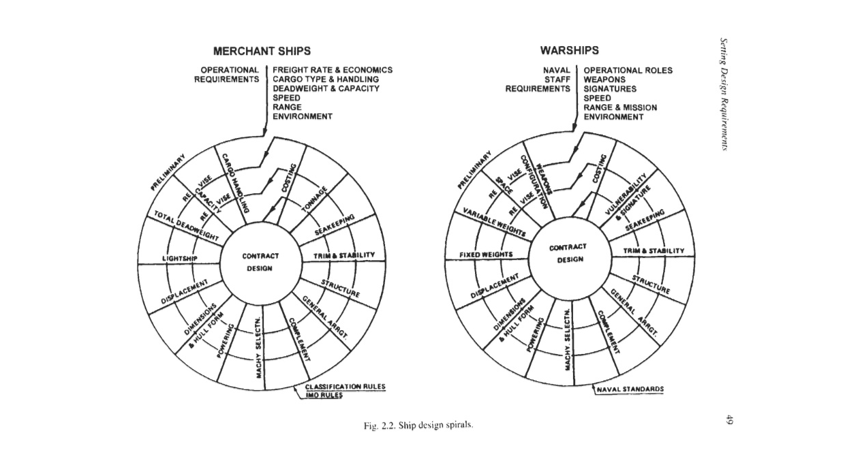
\includegraphics[width=1\linewidth]{CHAPTER 2/WarShip Design Spiral.png}
        \caption{WarShip Design Spiral \cite{watson_practical_ship_design}}
        \label{fig:my_label}
    \end{figure}
   \subsection{The Payload Analysis Approach}
   To overcome the limitations of parent ship analysis, this project adopts the Payload Analysis Method (also known as the First-Principles / Weight-Volume Approach) to fix the main dimensions of our stealth corvette. \vspace{\baselineskip} \par\noindent Instead of guessing hull dimensions first and fitting equipment inside later, Payload Analysis works from the inside out:
   \begin{enumerate}[\alph*)]
       \item\textbf{Weapon and Mission Systems Identification: } We establish the exact tactical payload required for the mission profile (e.g., BrahMos VLS, SAM arrays, torpedo bays, towed array sonars, aviation facilities, and radar suites).
       \item \textbf{Weight and Space Estimation:}The physical weight, structural margins, power demands, and volumetric footprint of every weapon and sensor system are cateloged.
       \item \textbf{Crew and Logistics Allocation: } Required crew complements, living spaces, fresh water, and fuel oil capacities for a 4,000 nautical mile endurance are calculated based on naval habitability standards.
       \item \textbf{Hull Sizing Iteration:}Using parametric weight-displacement relationships, the total required displacement $(\Delta)$ is derived. From these baseline requirements, the final principal dimensions (L,B,D,T) are calculated to ensure the hull provides sufficient buoyancy, stability, and volumetric capacity.
   \end{enumerate}
   By anchoring our design in Payload Analysis, we ensure that the fixed principal dimensions are tailored directly to our corvette’s specific operational needs .
   \section{Mission Analysis}
   A Next-Generation Corvette is built as a flexible, multi-role warship designed to bridge the gap between heavy open-ocean frigates and small coastal patrol craft.
   \vspace{\baselineskip} \par\noindent Its primary functions are high lethality, operational stealth, and tactical adaptability.
   \begin{enumerate}[\alph*)]
       \item \textbf{Primary Role :}Anti-Submarine Warfare (ASW), Anti-Surface Warfare (ASuW), Local Air Defence, Maritime Surveillance\& EEZ Patrol, Mine Warfare Support.
       \item \textbf{Secondary Role :}Maritime Security, Coastal Defence, Convoy Escort, Search \& Rescue, and Humanitarian Assistance \& Disaster Relief (HADR).
   \end{enumerate}
    \section{Payload Selection}
    The Payload Selection Approach is a "bottom-up" engineering methodology designed specifically for warships, which are fundamentally weight- and volume-driven platforms rather than cargo-driven ones. Instead of guessing the size of the hull first and trying to fit equipment in it, this approach begins with the payload of the core mission payload—cataloging the exact weights, physical dimensions, power draws, and operational space requirements of all tactical systems (such as vertical launch missile cells, main guns, radar suites, sonar arrays, and aviation facilities). Once the combat system envelope is established, secondary requirements are built around it, calculating the necessary propulsion plant, electrical power generation, fuel and fresh water reserves for target endurance, and accommodation for the crew. \vspace{\baselineskip} \par.\noindent By aggregating these payload and support demands, naval architects calculate the total required structural displacement and internal volume. From this bottom-line volumetric requirement, the principal hull dimensions—length, beam, depth, and draft—are derived using hydrostatic and hydrodynamic equations. This ensures that the finalized hull is neither under-sized, which would compromise combat effectiveness and stability, nor over-sized, which would unnecessarily inflate construction costs, hydrodynamic resistance, and radar cross-section. Ultimately, the payload approach creates a tightly integrated, customized warship where every meter of hull space directly serves an operational purpose.
    \subsection{Main Deck Naval Artillery}The main gun on a warship serves as its primary medium-caliber kinetic weapon system, mounted on the forward deck to provide automated rapid-fire support against surface ships, low-altitude aerial threats, and shore targets. Directed by the ship's fire-control radar, it balances kinetic firepower with multi-domain versatility.
    \vspace{\baselineskip}\par\noindent
    OTO Melara 76/62 mm Super Rapid is the ideal selection for a corvette because it delivers an exceptional balance of low weight, extreme rate of fire, and multi-role versatility without overloading the hull's displacement. 
    
    \vspace{\baselineskip}\par\noindent
    Weighing less than 8 ton compared to 25+ tons for 127 mm guns, it preserves the ship's forward center of gravity while offering a rapid firing rate of up to 120 rounds per minute, allowing it to double as a effective close-in defense system against anti-ship missiles, aircraft, and drone swarms. \vspace{\baselineskip}\par\noindent Furthermore, its radar-absorbent stealth cupola seamlessly integrates into our vessel’s low-RCS geometry, its compatibility with smart guided ammunition (like STRALES and VULCANO) provides extended-range precision strike capability, and its established domestic manufacturing (via BHEL) guaranties low lifecycle costs and seamless integration with indigenous combat management systems.
    \begin{figure}[htbp]
        \centering
        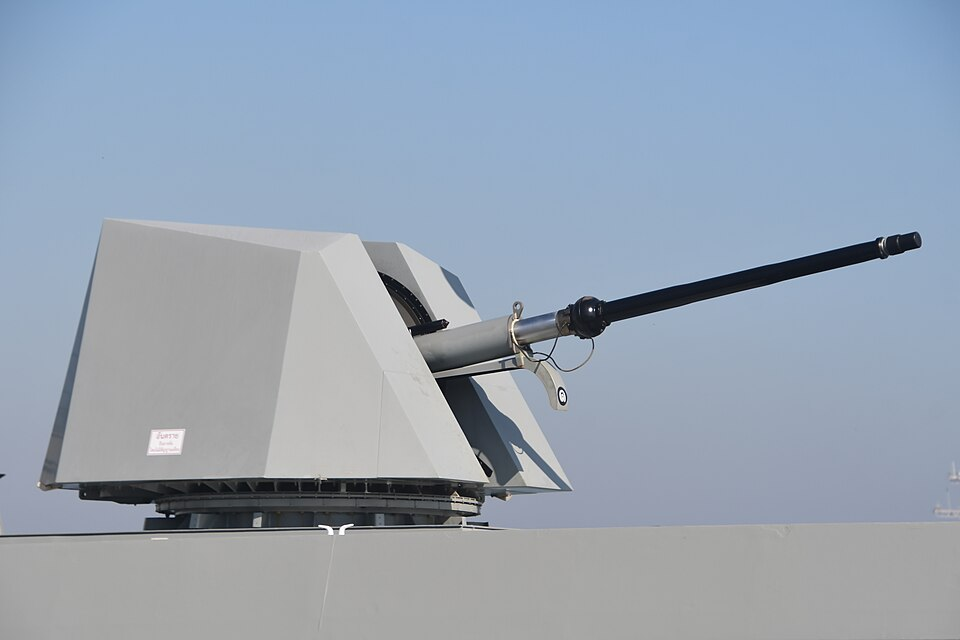
\includegraphics[width=0.5\linewidth]{CHAPTER 2/Oto_Melara_76mm_Super_Rapid_Gun_mount_on_HTMS_Bhumibol_Adulyadej_(FFG-471)_right_front_view_at_JMSDF_Yokosuka_Naval_Base_November_3,_2022_01.jpg}
        \caption{OTO Melara 76/62 mm Super Rapid Main Deck Naval Gun}
        \label{fig:placeholder}
    \end{figure}
    \subsection{Anti-Surface Warfare (ASuW) Missile System} 
    Anti-Surface Warfare (ASuW) systems serve as a warship's primary offensive strike weapon, designed to neutralize hostile surface combatants, heavily armored fleet formations, and strategic coastal land targets at beyond-visual-range (BVR) distances. Modern naval ASuW relies on long-range cruise missiles launched from vertical launch system (VLS) cells or deck-mounted angled canisters, guided by active radar seekers, satellite navigation, and mid-course data links to execute precision sea-skimming attacks.
    \begin{figure}[htbp]
        \centering
        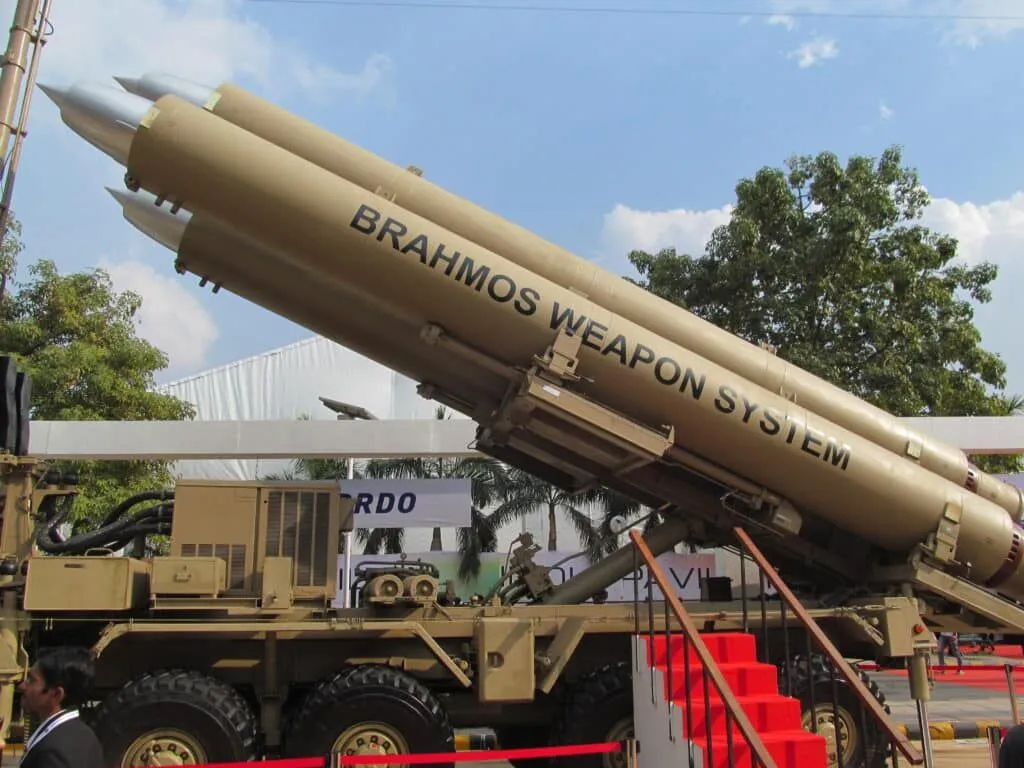
\includegraphics[width=0.5\linewidth]{CHAPTER 2/Brahmos Quad Launching System.png}
        \caption{Brahmos Quad Launching System \cite{csis2024brahmos}}
        \label{fig:placeholder}
    \end{figure}
    \par\noindent The BrahMos supersonic cruise missile is the premier choice for corvette's primary ASuW capability because its unmatched Mach 2.8 to Mach 3.0 speed and sea-skimming trajectory leave target ships with virtually zero reaction time, making defense interception practically impossible. By opting for an 8-cell Universal Vertical Launch System (UVLS) integrated flush into the forward deck, we preserve the ship's low Radar Cross-Section (RCS) while avoiding the exposed weight and drag of traditional inclined deck launchers.

    \subsection{Surface-to-Air Missile (SAM) System}
    Naval Surface-to-Air Missile (SAM) systems serve as a warship's primary defensive shield against airborne threats, including high-speed anti-ship sea-skimmer missiles, strike aircraft, helicopters, and unmanned aerial vehicles (UAVs). Modern naval SAM systems rely on vertical launch systems (VLS) for rapid $360^{\circ}$ coverage, using active radar homing seekers and mid-course guidance to track and destroy incoming threats before they reach the ship's outer defense perimeter.
    \begin{figure}[htbp]
        \centering
        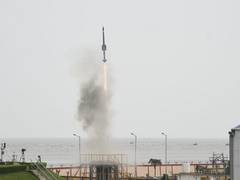
\includegraphics[width=0.5\linewidth]{CHAPTER 2/VL-SRSAM Vertical Launch Test for Naval Surface Defence.png}
        \caption{VL-SRSAM Vertical Launch Test for Naval Surface Defence \cite{ani2024vlshorads}}
        \label{fig:placeholder}
    \end{figure}
    \par\noindent The indigenous VL-SRSAM is the most suitable air-defence system for our stealth corvette because its compact vertical-launch design provides true $360^{\circ}$ rapid-reaction coverage against high-speed sea-skimming anti-ship missiles without the mechanical slew delays or blind spots associated with older trainable arm launchers. Using a 16-cell canisterized VLS module integrated flush into the superstructure, it eliminates topside structural weight, protects the missiles from harsh marine environments, and preserves the low Radar Cross-Section (RCS).
    \subsection{Close-In Weapon System (CIWS)} A Close-In Weapon System (CIWS) acts as a warship's final point-defense line of kinetic protection against fast-approaching threats that have penetrated the outer envelope of the SAM missile. Typically featuring fully automated, high-rate-of-fire rotary cannons slaved to dedicated radar and optronic trackers, a CIWS detects, locks onto, and destroys incoming sea-skimming anti-ship missiles, low-flying aircraft, guided munitions, and hostile drone swarms at close range (1 to 4 km) using a dense wall of high-explosive or armor-piercing artillery.
    \begin{figure}
        \centering
        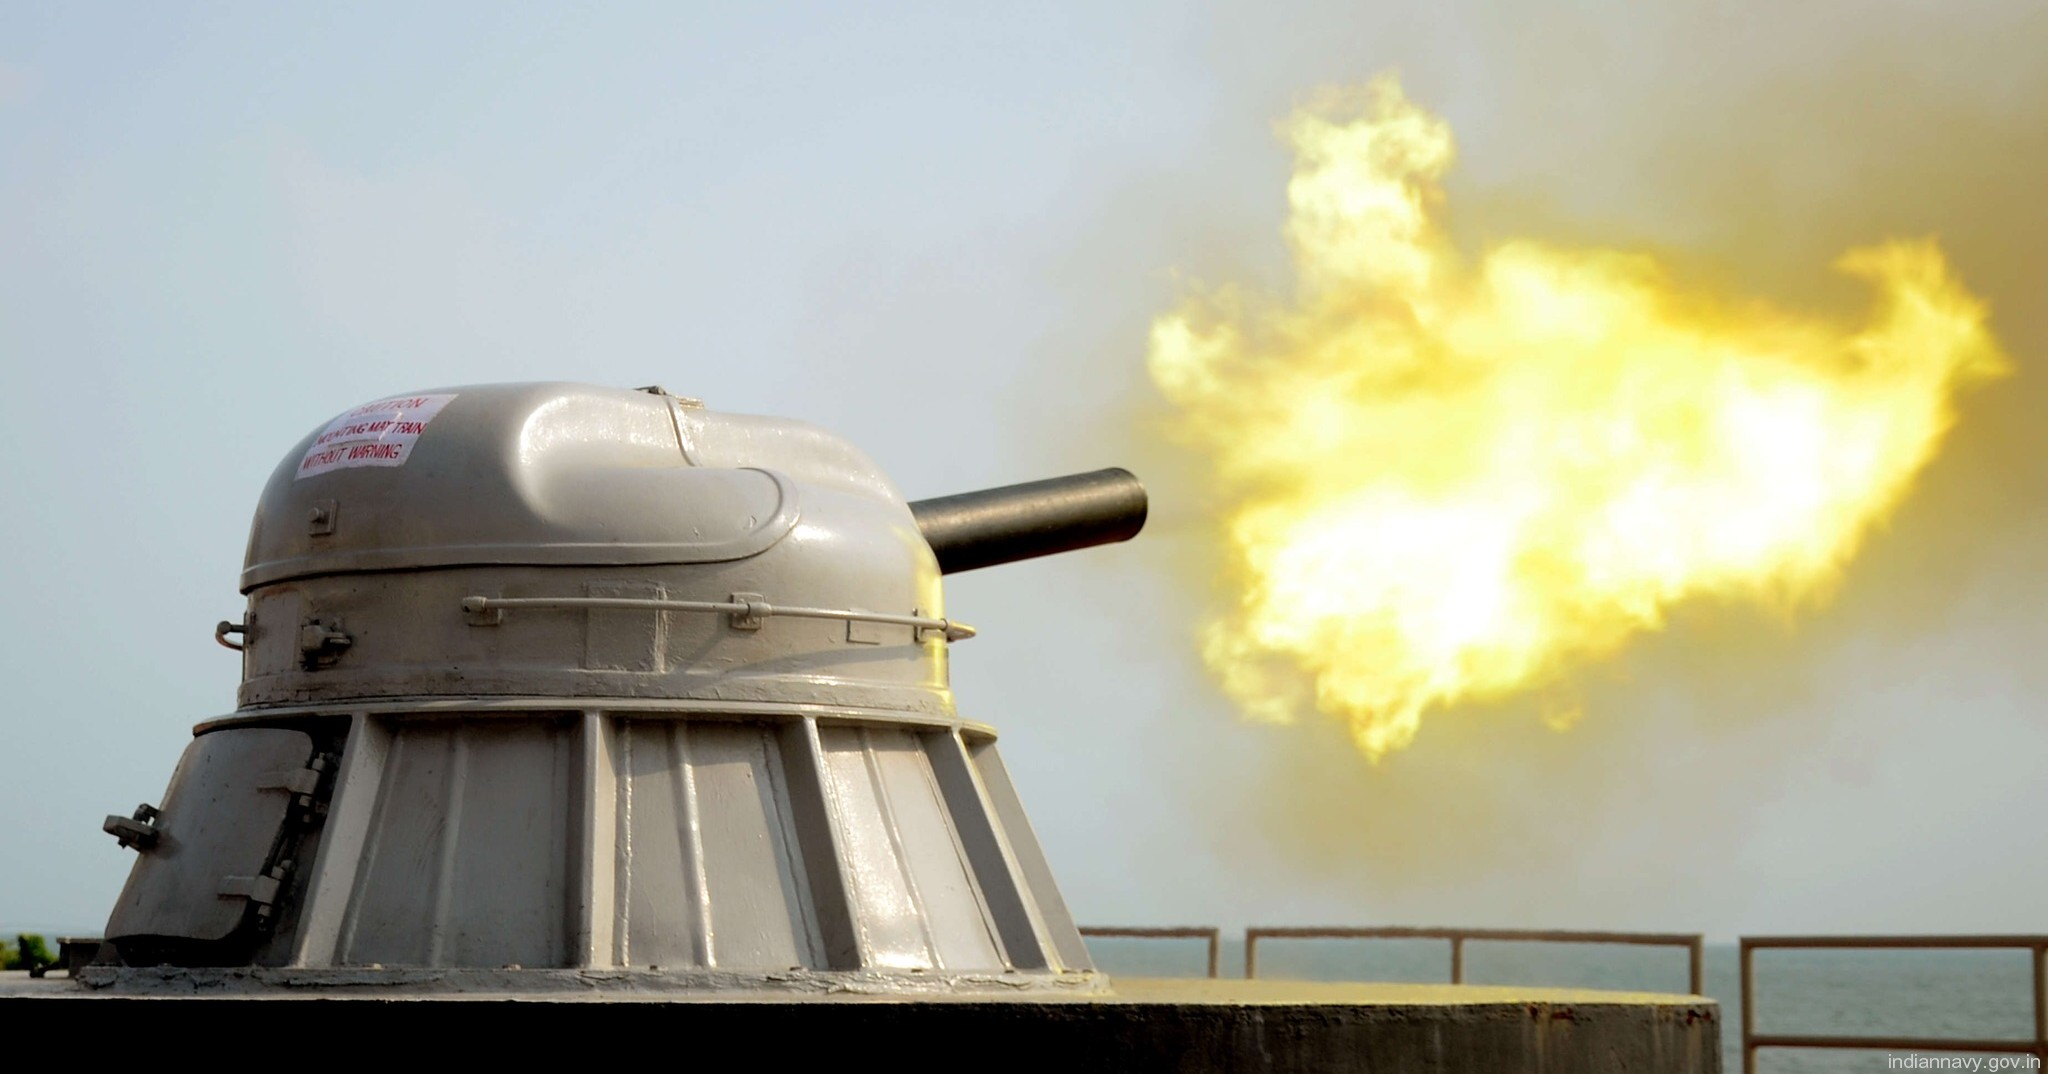
\includegraphics[width=0.5\linewidth]{CHAPTER 2/AK-630M 30mm Close-In Weapon System (CIWS.png}
        \caption{AK-630M 30mm Close-In Weapon System (CIWS) \cite{seaforces_ak630}}
        \label{fig:placeholder}
    \end{figure}
    \par\noindent The AK-630M is the most suitable CIWS choice for stealth corvette because its 6-barrel 30"mm"  rotary cannon delivers an intense firing rate of up to 5,000 rounds per minute, creating a high-density fragmentation screen capable of physically shredding incoming supersonic anti-ship missiles at close ranges. Its compact turret configuration allows dual mounts to be positioned laterally or aft on the superstructure deck without imposing heavy structural loads or displacing internal VLS spaces.
    \subsection{Anti-Submarine Warfare (ASW) Torpedo System} An Anti-Submarine Warfare (ASW) torpedo system forms a warship's primary underwater strike capability, designed to detect, track, and destroy quiet conventional or nuclear submarines in both shallow littoral waters and deep ocean environments. Launched via shipborne twin or triple tubes mounted at the beam, modern heavy/lightweight torpedoes utilize active/passive acoustic homing, conformal arrays, and wire-guidance feedback to maneuver autonomously, counter acoustic decoys, and detonate high-explosive warheads directly against a submarine's pressure hull.
    \begin{figure}[htbp]
        \centering
        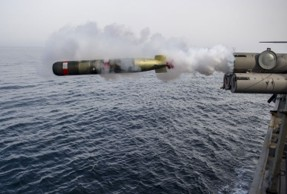
\includegraphics[width=0.5\textwidth]{CHAPTER 2/TAL SHYENA.jpg}
        \caption{TAL Shyena Launch System \cite{kattoch2020torpedoes}}
        \label{fig:TAL SHYENA IMAGE}
    \end{figure}
    \par\noindent The indigenous TAL Shyena is considered suitable for our corvette's primary ASW requirement because    of its compact size, relatively low weight, and ability to operate at considerable underwater depths. The torpedo has a diameter of 324 mm, a length of approximately 2.752 m, and a warhead weight of approximately 220 kg. It is electrically propelled using a seawater-activated battery and can attain a maximum speed of approximately 33 knots, with an endurance of approximately 6 minutes. The system has an operating depth of up to 450 m, allowing it to engage submarines operating in a wide range of underwater conditions.
    \subsection{Modular Multi-Role Mission Bay}
    A midship mission bay is a dedicated, reconfigurable internal space positioned at the ship's center of gravity, designed to accommodate modular equipment, auxiliary craft, and specialist payloads. Featuring overhead davits, internal crane tracks, and hydraulic side-launch doors, it enables the safe deployment and recovery of Rigid-Hull Inflatable Boats (RHIBs), Unmanned Surface Vessels (USVs), and Autonomous Underwater Vehicles (AUVs) while protecting them from severe weather.
    \begin{figure}
        \centering
        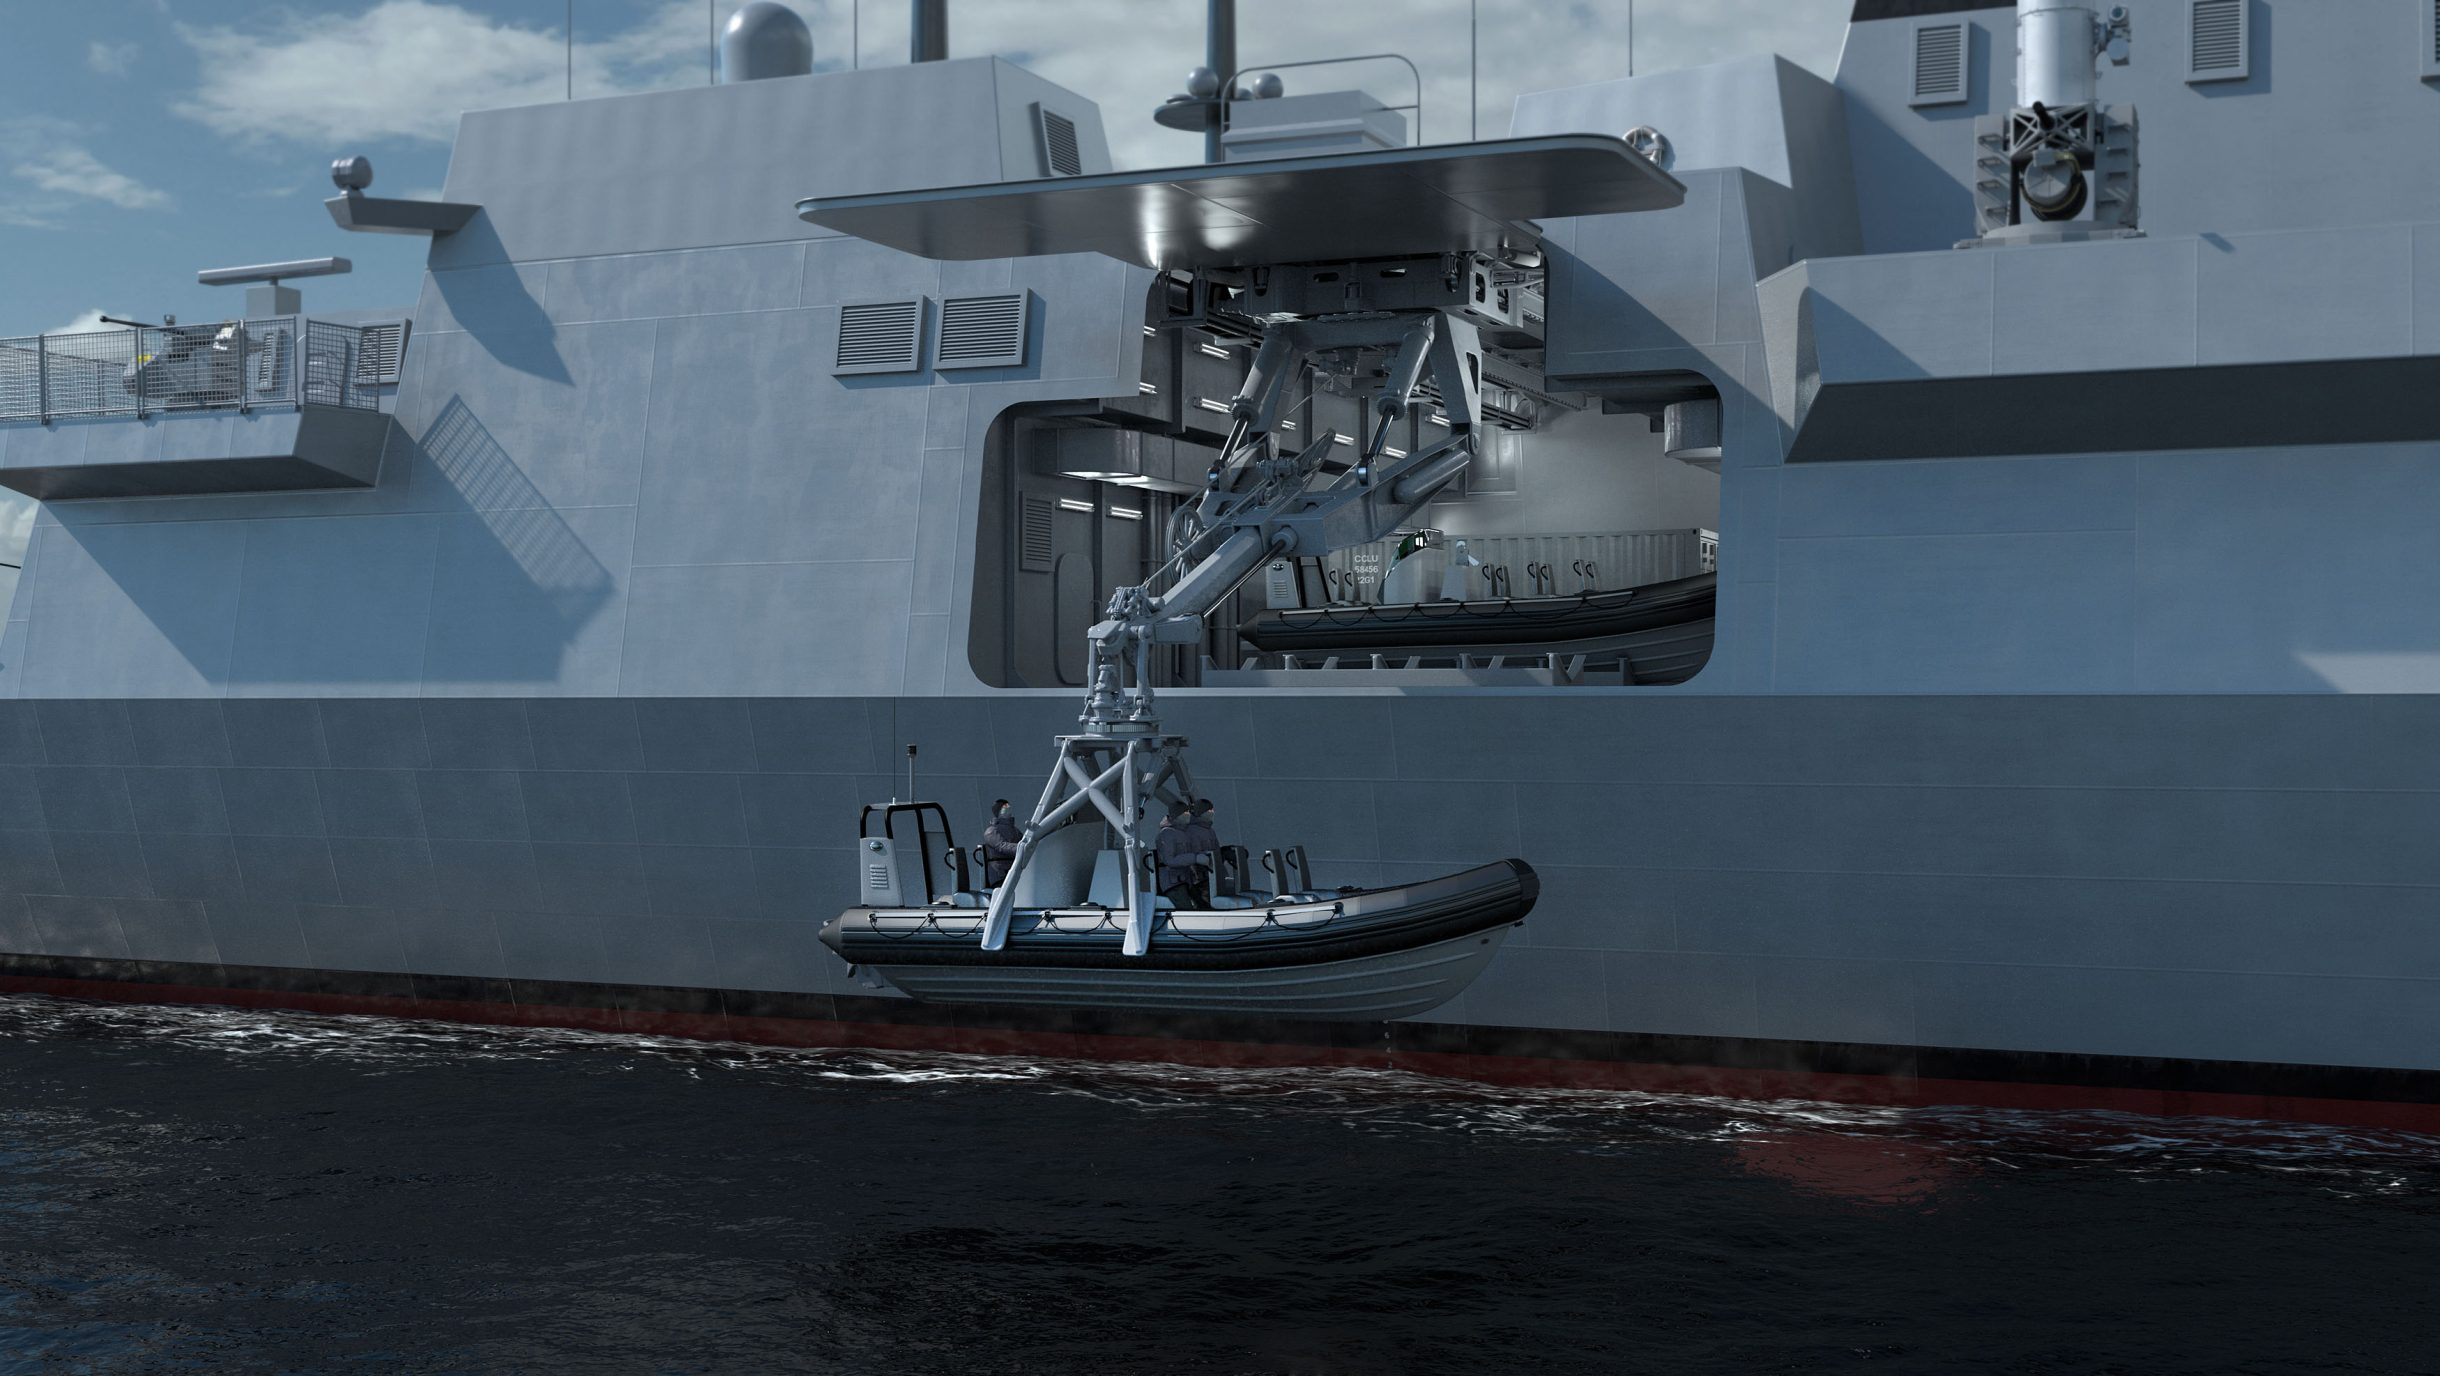
\includegraphics[width=0.5\linewidth]{CHAPTER 2/Mission Bay Handling System.png}
        \caption{Mission Bay Handling System \cite{fmd_missionbayhandling}}
        \label{fig:placeholder}
    \end{figure}
    \subsection{Primary Surveillance Radar}
    The primary surveillance radar serves as the ship's main multi-function electronic "eye," providing continuous 3D air and surface tracking, target classification, and weapons guidance.
    
    \par\noindent Operating in the S-band, modern naval Active Electronically Scanned Array (AESA) systems use multiple fixed solid-state antenna panels to sweep $360^{\circ}$ electronically without moving parts, simultaneously detecting high-altitude strike aircraft, low-observable sea-skimming anti-ship missiles, and surface vessels.
    \begin{figure}[htbp]
        \centering
        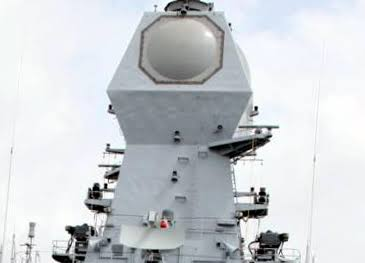
\includegraphics[width=0.5\linewidth]{CHAPTER 2/MF-STAR Multi-Function AESA Surveillance Radar.jpg}
        \caption{EL/M-2248 MF-STAR Multi-Function AESA Surveillance Radar \cite{namu_m2248}}
        \label{fig:placeholder}
    \end{figure}
   \vspace{\baselineskip}\par\noindent The EL/M-2248 MF-STAR is the ideal choice for primary surveillance on our corvette because its scalable, 4-panel fixed AESA architecture provides continuous 360-degree tracking and instantaneous multi-beam guidance for air-defense missiles without mechanical rotation delays. In its compact corvette configuration (weighing roughly 3.3 tons), it fits comfortably on the main mast, minimizing top-weight while delivering detection ranges out to 250 km for aircraft and over 25 km against fast, low-RCS sea-skimmers.
   \subsection{Secondary Underwater Surveillance (Sonar)}The primary subsurface surveillance suite on a surface combatant relies on a Hull-Mounted Sonar (HMS) housed in a bulbous bow dome beneath the waterline. It operates in dual active and passive modes to transmit low-to medium frequency acoustic pulses through the water column, listening for echo returns to detect submerged submarines, incoming torpedoes, and underwater obstacles in both shallow littoral waters and deep ocean environments.
   \par\noindent The indigenous is the most suitable underwater sensor for our corvette because its advanced digital processing and adaptive beam-forming algorithms give it exceptional active/passive tracking range against quiet conventional submarines in noisy, high-clutter Indian Ocean waters. Developed by NPOL/DRDO and manufactured by BEL, its compact transducer array fits neatly into our vessel's bow dome without causing excessive hydrodynamic drag or compromising high-speed performance.
   \subsection{Soft-Kill Decoy System}A naval soft-kill decoy system serves as a warship's primary electronic countermeasure defense against incoming radar-guided anti-ship missiles. Rather than physically intercepting threats with kinetic artillery or surface-to-air missiles, it launches rocket-borne chaff cartridges that bloom into suspended, highly radar-reflective clouds.
   \begin{figure}
       \centering
       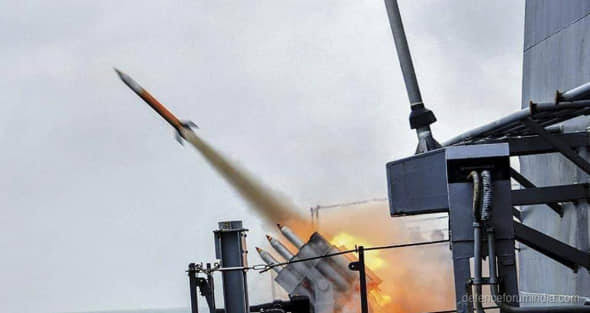
\includegraphics[width=0.5\linewidth]{CHAPTER 2/Kavach Chaff Rocket Decoy System for Naval Electronic Defence..png}
       \caption{Kavach Chaff Rocket Decoy System for Naval Electronic Defence. \cite{nextgenerationweapons_kavach}}
       \label{fig:placeholder}
   \end{figure}
   \par\noindent The indigenous Kavach chaff decoy system is the most suitable soft-kill countermeasure for our 2,200-ton stealth corvette because its multi-layered defense capability operating in Long-Range Confusion, Medium Range Distraction, and Short-Range Seduction modes provides a comprehensive soft-kill shield against advanced sea-skimming anti-ship missile swarms.
   \section{Determination Of Principal Dimensions}To establish the preliminary length overall of the stealth corvette using the Payload-Driven Approach, a spatial allocation method is applied across the main weather deck. Rather than relying solely on empirical coefficients derived from historical ships, this method directly maps the functional footprint of every primary deck weapon, sensor mast, aviation facility, and operational clearance required along the ship's centerline.
   \subsection{Determination of Principal Length}The overall deck of the ship is divided into 3 main segments, they are:
   \begin{enumerate}[\alph*)]
       \item \textbf{Forward Section}The forward segment begins with a 10.0 m cut-off distance from the stem/bow apex to the mid of the main deck artillery. This length provides the necessary hydrodynamic bow overhang, fine entry lines to minimize wave-making resistance, anchor handling arrangements, and structural wave-breaker clearances. Immediately aft sits the OTO Melara 76/62 mm Super Rapid main gun, occupying a 4.5 m longitudinal footprint inclusive of its lower turret deck ring and service maintenance perimeter. To complete the forward strike zone, a 16-cell VL-SRSAM surface-to-air missile launcher is positioned in a 6.0 m module space directly behind the main gun, ensuring dedicated structural isolation from the forecastle.
       \begin{figure}[htbp]
       \centering
       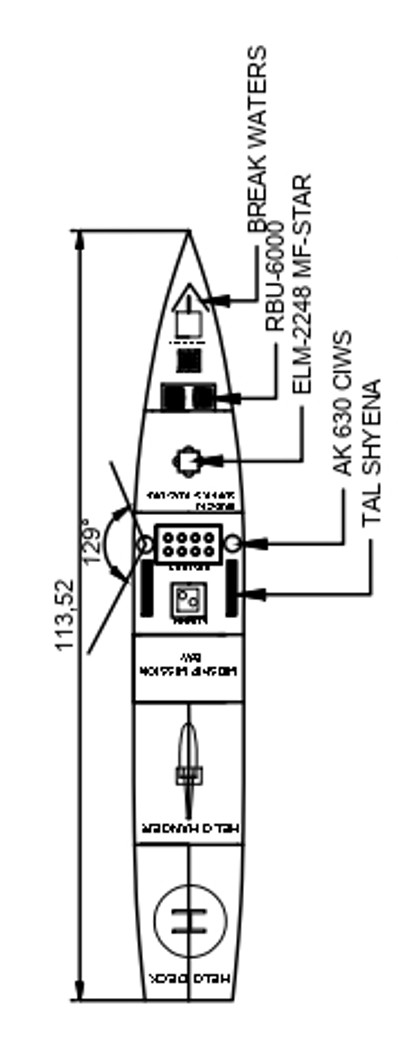
\includegraphics[width=0.4\textwidth]{CHAPTER 2/deck layout.jpg}
       \caption{Preliminary Deck Layout}
       \label{fig:preliminary deck layout}
   \end{figure}
       \item \textbf{Midship Section}The midship portion houses the ship's primary operational superstructure and machinery exhaust casings. A 15.0 m central superstructure module encompasses the enclosed navigation bridge, combat information centre (CIC), and the multi-function radar mast housing the EL/M-2248 MF-STAR AESA arrays. Directly adjoining this is a 22.5 m main machinery and payload zone, which contains the main engine uptakes and funnel enclosure, the Kavach chaff decoy launchers, and the 533"mm"  ASW torpedo launch tubes. To maximize volumetric efficiency and stealth, an internal 10.0 m modular midship mission bay is integrated directly underneath this funnel and torpedo zone, utilizing the central region of the hull for optimal transverse stability during offboard craft launch and recovery.
       \item \textbf{Aft Section}The aft deck architecture is dedicated entirely to aviation and multi-role operations. A 21.0 m enclosed helicopter hangar is provisioned to accommodate, store, and maintain a medium-class naval utility helicopter (such as the MH-60R or ALH Dhruv) alongside aviation fuel tanks and weapons storage. Extending to the stern is a 23.0 m helicopter flight deck. Beyond providing a safe landing zone with adequate deck margin for high sea-state flight operations, this expansive aft deck provides flexible operational area for Replenishment at Sea (RAS) transfers, board-and-search staging, and vertical replenishment (VERTREP).
   \end{enumerate}
   
   \vspace{\baselineskip}\par\noindent  From Figure \ref{fig:preliminary deck layout}  summating these discrete structural and operational zones, the initial baseline length for the weather deck is established at 114 m.Therefore \par\noindent$$\textbf{L}_{pre} = 114m$$.
   \subsection{Determination of Principal Breadth}Determining the molded breadth (beam) of the stealth corvette requires an inside-out spatial sizing process driven by the internal envelope of the enclosed midship mission bay. Because the hull must accommodate various primary combat systems, internal machinery casings, and uncrewed vehicles offboard within a streamlined stealth profile, the minimum width of the vessel is dictated directly by the transverse arrangement of these mission-critical assets. \begin{figure}[htbp]
       \centering
       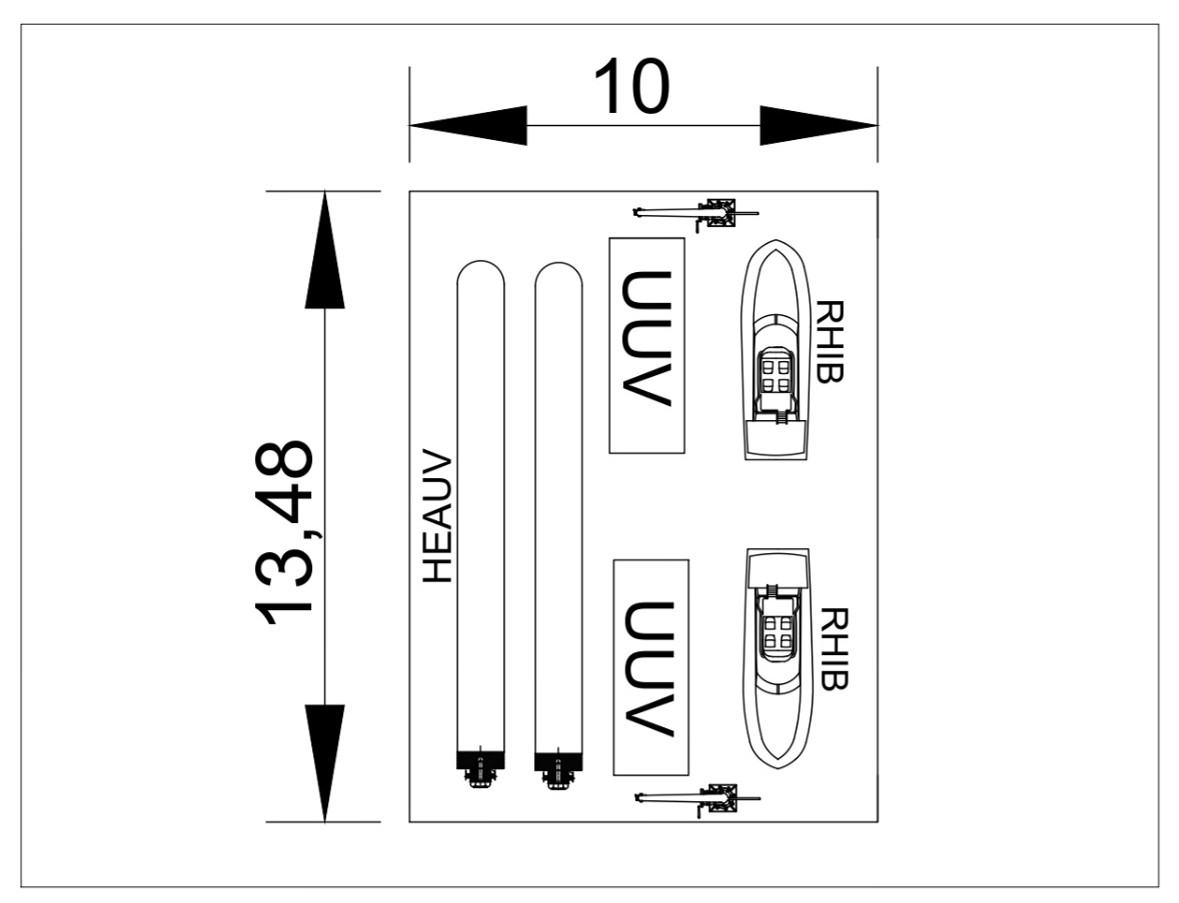
\includegraphics[width=0.7\linewidth]{CHAPTER 2/preliminary miship bay.jpg}
       \caption{Preliminary Midship Mission Bay}
       \label{fig:preliminary mission bay}
   \end{figure}
   \vspace{\baselineskip}\par\noindent The core driver for this beam constraint is the multi-role midship mission bay, which houses two Rigid-Hull Inflatable Boats (RHIBs), two Unmanned Underwater Vehicles (UUVs), and two Heavy Expeditionary Autonomous Underwater Vehicles (HEAUVs) alongside two dual-point hydraulic boat davits. To prevent operational congestion, allow rapid deployment during emergency board-and-search missions, and ensure that crew maintenance personnel can safely maneuver around parked systems.
  
   \par\noindent Consequently, 13.48 m is established as the baseline preliminary beam (B) at the waterline. This beam dimension guaranties that the mission bay remains ungested while simultaneously ensuring an optimal Length-to-Beam ratio, which maintains good hydrodynamic efficiency, high-speed stability, and adequate metacentric height ($GM_{T}$).$$\textbf{B}_{pre} = 14m$$.
   \section{Initial Complement Estimation}The total complement according to the OSR was given as 125, to accommodate a 10\% additional complement. An empirical approach is used for the initial estimate of the ships complement in various categories. The complement was drawn in officers and sailors. The margins and break up of the ship's crew is shown below. The initial estimate of the complement (N) is taken as 138. Compared to the graphs in the UCL Databook, the complement provided is less. This is mainly due to the inclusion of advanced equipment in modern ships. The number of complements and the distribution is shown in Table \ref{tab:complement}
\begin{table}[htbp]
\centering
\caption{Estimation of Complement}
\label{tab:complement}

\begin{tabular}{lcc}
\toprule
\textbf{Personnel Requirement} & \textbf{UCL Proportions} & \textbf{Number} \\
\midrule
N         & $N$       & 138 \\
Officers  & $0.075N$  & 11  \\
CPO       & $0.110N$  & 15  \\
PO        & $0.140N$  & 20  \\
JR.       & $0.675N$  & 92  \\
\bottomrule
\end{tabular}

\vspace{2mm}

\footnotesize
\textit{Source: UCL Ship Design Data Book, 2011. \cite{ucl_ship_design_data_book}}

\end{table}
\section{Initial Displacement and Volume Estimation}The total hull volume and weight was assumed to be divided into seven weight groups as shown below. The weight and volume under each of these seven heads were calculated as per the guidelines. They are mainly categorized as follows:
\begin{enumerate}[\alph*)]
    \item \textbf{Hull : }The Hull group includes the structural components of the ship such as shell plating, decks, bulkheads, frames, girders and superstructure. It also accounts for the structural weight required to provide adequate strength and support for the ship.
    \item \textbf{Personnel : }The Personnel group includes the accommodation and provisions associated with the ship's crew. It covers personnel-related spaces, furnishings, clothing, personal equipment and other requirements necessary for crew operation.
    \item \textbf{Ship Systems : }The Ship Systems group comprises the various services required for the safe and effective operation of the vessel. These include piping, ventilation, air-conditioning, fire-fighting, damage-control and other auxiliary ship services.
    \item \textbf{Propulsion : }The Propulsion group includes the main machinery and associated equipment required to generate and transmit power for ship propulsion. It includes prime movers, gearboxes, shafting, propellers and related propulsion auxiliaries.
    \item \textbf{Electricals : }The Electrics group covers the equipment required for generation, distribution and utilisation of electrical power onboard. This includes generators, switchboards, transformers, cables, batteries and associated electrical equipment.
    \item \textbf{Payload : }The Payload group represents the mission-specific equipment and load carried by the ship. For a corvette, this may include weapons, ammunition, sensors, communication systems and other operational equipment specified by the mission requirements.
    \item  \textbf{Variables (Stores and Fuel) : }The Variables group consists mainly of consumable loads that change during the ship's operation. It includes fuel, lubricating oil, fresh water, provisions, stores, ammunition expenditure and other variable consumables.

    \vspace{\baselineskip}\par \noindent These descriptions are consistent with the UCL seven-group weight system, which is intended to organize the preliminary estimates of ship weight, space and power during the design process.

   \vspace{\baselineskip}\par \noindent For your corvette report, I would use these exactly as written because they are formal enough for a technical report while remaining short enough to fit the large blank spaces shown in your screenshot.
\end{enumerate}

\vspace{\baselineskip}\par \noindent Using open-source technical data , the weights of the payload components of the ship were collated into a comprehensive baseline table \ref{tab:equipment_weight}, resulting in an initial payload weight of 121.22 tons. To account for future system growth, structural interfaces and design contingencies, a margin was applied, establishing the final payload weight of the design at 145.46 tons.
\begin{table}[H]
\centering
\caption{Preliminary Equipment Weight Estimate}
\label{tab:equipment_weight}
\begin{tabular}{l r r}
\midrule
\textbf{Equipment} & \textbf{Quantity} & \textbf{Weight (t)} \\
\midrule
OTO Melara 76 mm \cite{seaforces_otomelara76} & 1 & 8.0153 \\
Vertical Launching System \cite{seaforces_mk57} & 16 & 19.331 \\
VL-SRSAM \cite{bdl_vlsrsam}& 16 & 2.72 \\
BrahMos \cite{csis2024brahmos}& 8 & 12 \\
Quad Launching \cite{csis2024brahmos} & 2 & 6.00 \\
TAL Shyena \cite{bdl_tal} & 6 & 1.185 \\
HEAUV \cite{kodainya_drdoheauv}& 2 & 12.00 \\
AK-630 \cite{navweaps_ak630}& 2 & 3.782 \\
ELM-2248 MF-STAR \cite{radartutorial_naval_radar}& 1 & 3.30 \\
Kelvin Hughes \cite{hensoldt_sharpeye_mk11}& 1 & 0.80 \\
HUMSA-NG \cite{bel_humsang_mk2}& 1 & 5.00 \\
HAL Dhruv \cite{hal_dhruv}& 1 & 5.80 \\
RHIB \cite{shmgroup_product_catalogue}& 2 & 7.00 \\
UUV \cite{shmgroup_product_catalogue} & 1 & 2.00 \\
Davit \cite{viking_offshore_lifeboats}& 2 & 22.40 \\
RBU-6000 \cite{weaponsystems_rbu6000}& 2 & 9.068 \\
VisionMaster \cite{manualslib_visionmaster_ft}& 1 & 0.044 \\
Garpun \cite{deagel_3ts25e}& 1 & 1.00 \\
Selesmar & 1 & 1.086 \\
BridgeMaster \cite{bmemarine_bridgemaster_e}& 1 & 0.10 \\
ELLORA \cite{mod2007annualreport}& 1 & 1.00 \\
\multicolumn{2}{l}{{Fire Control Systems}} & 18.00 \\
\multicolumn{2}{l}{{Navigation Systems}} & 1.01 \\
\multicolumn{2}{l}{{Communication Systems}} & 1.35 \\
\multicolumn{2}{l}{{Deck Handling Equipment}} & 25.00 \\
\multicolumn{2}{l}{{Firefighting \& Damage Control}} & 8.50 \\
\multicolumn{2}{l}{{Aviation Support}} & 10.50 \\
\multicolumn{2}{l}{{UUV Support}} & 3.00 \\
\multicolumn{2}{l}{{Spares \& Special Tools}} & 10.00 \\
\midrule
\multicolumn{2}{l}{{Total Weight}} & \textbf{200.991} \\
\multicolumn{2}{l}{{Design Margin (10\%)}} & \textbf{20.0991} \\
\multicolumn{2}{l}{\textbf{Final Weight}} & \textbf{221.09} \\
\midrule
\end{tabular}
\end{table}
Based on the calculated payload displacement, the required payload volume was determined. Typically, the payload density was assumed to be 0.9 $t/m^{3}$, and the total payload volume for the vessel was evaluated to be 394.4$m^3$.
The volume of the underwater hull ($\nabla$) of the vessel is estimated using the product of the length between the perpendiculars (L), the width of the molded (B), the design draft (T) and the block coefficient ($C_B$). For corvette-sized combatants, the block coefficient typically ranges from 0.35 to 0.60. Adopting a design $C_B$ of 0.54, along with the principal dimensions of L=114 m, B=14 m and an assumed design draft of T=5.00 m, the preliminary design is adopted. 

    
The displacement volume is evaluated as follows:
\begin{equation}
V_{\text{Estimated}} = L \times B \times T \times C_B
\label{eq:estimated_volume}
\end{equation}
\addcontentsline{loe}{equations}{Estimated Volume}

$$= 114 \times14\times5\times0.54$$
$$=4.309.2m^{3}$$
 Before evaluating the final volumetric and displacement estimates, the UCL Ship Design Procedure requires specific design margins to account for weight growth, space integration allowances, and future equipment additions across each functional system category. These design margins, applied to both weight and spatial allocations, are summarized in Table \ref{tab:design_margins} below.
\begin{table}[htbp]
    \centering
    \caption{Designer, board, and growth margins for weight and spatial allocation.}
    \label{tab:design_margins}

    \begin{tabular}{lccccc}
        \toprule
        \textbf{Group} &
        \multicolumn{2}{c}{\textbf{Designer Margin}} &
        \multicolumn{2}{c}{\textbf{Board Margin}} &
        \multicolumn{1}{c}{\textbf{Growth Margin}} \\
        
        & \textbf{W (\%)} & \textbf{V (\%)} &
        \textbf{W (\%)} & \textbf{V (\%)} &
        \textbf{W (\%)} \\
        \midrule
        
        Hull        & 5 & -- & 2 & -- & 5 \\
        Personnel   & -- & 5 & 2 & -- & 5 \\
        Ship Systems & 5 & 2 & 2 & -- & 5 \\
        Machinery   & 4 & -- & 2 & -- & 5 \\
        Electrical  & 5 & -- & 5 & 5 & 5 \\
        Payload     & 7 & 10 & 2 & -- & 5 \\
        Variables   & 4 & 4 & 2 & -- & 5 \\
        
        \bottomrule
    \end{tabular}

    \vspace{2mm}
    
    \footnotesize
    \textit{Source: UCL Ship Design Data Book, 2011. \cite{ucl_ship_design_data_book}}
    
\end{table}
In accordance with the UCL Ship Design Methodology, each primary system category is further subdivided into specific warship functional groups to ensure complete weight accounting. Detailed weight calculations were performed in Excel to compute the baseline masses in all constituent groups. The applicable category-specific margins (as described in Table \ref{tab:design_margins}) were individually applied to each group's base weight. Summing these margined category weights yields the preliminary baseline displacement. Finally, a cumulative global design margin of 5\% was applied to the calculated baseline displacement to establish the total design displacement for the vessel.
\begin{table}[htbp]
    \centering
    \caption{Estimated displacement and margins for different weight groups.}
    \label{tab:displacement_margin}

    \begin{tabular}{lccc}
        \toprule
        \textbf{Category} &
        \textbf{Calculated Displacement (t)} &
        \textbf{Margin (\%)} &
        \textbf{Displacement (t)} \\
        \midrule

        Hull          & 1221 & 12 & 1211.291424 \\
        Personnel     & 195  & 7  & 194.4706853 \\
        Systems       & 568  & 12 & 546.5328512 \\
        Propulsion    & 400  & 15 & 460 \\
        Electricals   & 226.9565  & 15 & 261 \\
        Payload       & 220.09  & 14 & 250.90 \\
        Variable Loads & 621 & 11 & 611.7732353 \\
        \midrule
        \textbf{Total} & & & \textbf{3535.068} \\
        \bottomrule
    \end{tabular}

    \vspace{2mm}

    \footnotesize
    \textit{Source: Author's calculation based on the methods and equations given in the UCL Ship Design Data Book, 2011. \cite{ucl_ship_design_data_book}}

\end{table}
\subsection{Weight Estimations}
For the purpose of the present preliminary weight estimate, the adopted fixed-weight groups total approximately 2923.29t, while the variable-load component is 611.77t. Therefore, the preliminary lightship/fixed-weight estimate is approximately 2923.29t and the corresponding deadweight/variable-load estimate is approximately 611.77t. These values should be refined during subsequent design stages as detailed structural, machinery, equipment, fuel, and operational requirements are finalized.
\section{Parentship Analysis}

Before determining the preliminary principal dimensions of the proposed vessel,
a parametric study was carried out using existing naval vessels that had similar
operational characteristics and configuration. The principal dimensions and
relevant hull-form parameters of these vessels were collected and compared to
identify suitable ranges for the proposed design.

\begin{table}[htbp]
    \centering
    \caption{Parent Ship Analysis}
    \label{tab:parent_ship_analysis}

    \scriptsize
    \setlength{\tabcolsep}{3.5pt}

    \begin{tabular}{llccccccccc}
        \toprule
        \textbf{Country} &
        \textbf{Class} &
        \textbf{L (m)} &
        \textbf{B (m)} &
        \textbf{T (m)} &
        \textbf{$\Delta$ (t)} &
        \textbf{Speed (kn)} &
        \textbf{Range (nm)} &
        \textbf{$C_B$} &
        \textbf{L/B} &
        \textbf{B/T} \\
        \midrule

        Finland &
        Pohjanmaa \cite{pohjanmaa_rmc} &
        117 & 16.5 & 5.0 & 4300 & 26 & 3500 & 0.45 & 7.09 & 3.30 \\

        Russia &
        Steregushchiy \cite{steregushchiy_oni} &
        104.5 & 13 & 3.7 & 2200 & 27 & 3800 & 0.43 & 8.04 & 3.51 \\

        Algeria &
        Adhafer \cite{adhafer_c28a} &
        120 & 14.4 & 3.87 & 2880 & 30 & -- & 0.43 & 8.33 & 3.72 \\

        Russia &
        Gremyashchiy \cite{gremyashchiy_oni} &
        104.5 & 13 & 3.7 & 2430 & 27 & 4000 & 0.48 & 8.03 & 3.51 \\

        South Korea &
        Incheon \cite{incheon_helis} &
        114 & 14 & 4.0 & 3250 & 30 & 4500 & 0.51 & 8.14 & 3.50 \\

        Philippines &
        BRP Miguel Malvar \cite{miguel_malvar_pna} &
        118.4 & 14.9 & -- & 3200 & 25 & 4500 & 0.49 & 7.95 & -- \\

        Indonesia &
        Martadinata \cite{martadinata_class} &
        105.11 & 14.02 & 3.75 & 2946 & 28 & 5000 & 0.53 & 7.49 & 3.74 \\

        Brazil &
        Tamandaré \cite{tamandare_brazil_navy} &
        107.2 & 16.0 & 5.2 & 3455 & 25.5 & 5500 & 0.39 & 6.70 & 3.08 \\

        Egypt &
        Gowind-2500 \cite{gowind_egypt_alexandria} &
        102 & 16 & 3.6 & 2600 & 25 & 3700 & 0.33 & 6.38 & 4.44 \\

        \bottomrule
    \end{tabular}

    \vspace{2mm}

    \footnotesize
    \textit{Note: $C_B$ was calculated from displacement and principal dimensions.
    L/B and B/T were calculated from the corresponding dimensions.}

\end{table}
\subsection{First Estimate of Main DImensions}
Based on the preliminary layout of the deck, the initial displacement and other principal dimensions of the vessel were estimated. The dimensional and operational constraints specified in the OSR were then considered along with these preliminary values. Using these inputs, a Python-based computational code was developed to generate and evaluate different combinations of the principal dimensions, as presented in the Appendix~\ref{app:ship_dimension_generator}. The code calculates the corresponding displacement and hull-form parameters for each combination and identifies the feasible dimensions that satisfy the specified design constraints. This approach was used to systematically explore the available design space and select a suitable set of principal dimensions for further design calculations.
\vspace{\baselineskip}\par\noindent Among the feasible alternatives, the following dimensions are selected:
\begin{table}[htbp]
    \centering
    \caption{Preliminary Main Dimensions}
    \label{tab:preliminary_main_dimensions}

    \begin{tabular}{lc}
        \toprule
        \textbf{Parameter} & \textbf{Value} \\
        \midrule
        LOA          & 116 m \\
        B            & 16 m \\
        $L_{WL}$     & 113 m \\
        $B_{WL}$     & 15.04 m \\
        Draft        & 5.434 m \\
        Depth        & 10 m \\
        Displacement & 3600 t \\
        $C_B$        & 0.39 \\
        \bottomrule
    \end{tabular}
\end{table}
These values were selected because they give a displacement of 3650 tons, very close to the 3600-ton target, with a relatively fine block coefficient of 0.395 suitable for the 20-knot design speed. The resulting L/B and B/T ratios are within the range of the parent vessels, and the 10 m depth provides adequate freeboard without unnecessarily increasing the vessel depth. Therefore, it gives a balanced solution between displacement, high-speed hull form, stability, and practical arrangement requirements.
\section{Preliminary Power Estimation}
The propulsion power of the proposed vessel was initially estimated using a parent-ship regression method. Nine comparable naval vessels were selected based on their displacement, principal dimensions, and maximum speed. The displacement, maximum speed, and total installed propulsion power of the selected vessels were collected. A power-law relationship between propulsion power, displacement, and speed was assumed. The relationship was transformed into a linear form using logarithms and multiple linear regression was performed in Microsoft Excel.
\begin{table}[htbp]
    \centering
    \caption{Preliminary Power Estimation of Various Ships}
    \label{tab:preliminary_power_estimation}

    \footnotesize
    \setlength{\tabcolsep}{3.5pt}

    \begin{tabular}{lcccccc}
        \toprule
        \textbf{Vessel} &
        \textbf{$\Delta$ (t)} &
        \textbf{$V_{\max}$ (kn)} &
        \textbf{Power (kW)} &
        \textbf{$\ln(\Delta)$} &
        \textbf{$\ln(V)$} &
        \textbf{$\ln(P)$} \\
        \midrule

        Pohjanmaa \cite{pohjanmaa_rmc}
        & 4300 & 26 & 28000
        & 8.366370302 & 3.25809654 & 10.2399598 \\

        Steregushchiy \cite{steregushchiy_oni}
        & 2200 & 27 & 17600
        & 7.696212639 & 3.29583687 & 9.77565418 \\

        Adhafer \cite{adhafer_c28a}
        & 2880 & 30 & 23680
        & 7.965545573 & 3.40119738 & 10.0723861 \\

        Gremyashchiy \cite{gremyashchiy_oni}
        & 2430 & 27 & 17600
        & 7.795646536 & 3.29583687 & 9.77565418 \\

        Incheon \cite{incheon_helis}
        & 3300 & 30 & 56000
        & 8.101677747 & 3.40119738 & 10.933107 \\

        Miguel Malvar \cite{miguel_malvar_pna}
        & 3200 & 25 & 29600
        & 8.070906089 & 3.21887582 & 10.2955296 \\

        Martadinata \cite{martadinata_class}
        & 2946 & 28 & 20000
        & 7.988203597 & 3.33220451 & 9.90348755 \\

        Tamandaré \cite{tamandare_brazil_navy}
        & 3500 & 25.5 & 21280
        & 8.160518247 & 3.23867845 & 9.96552294 \\

        \bottomrule
    \end{tabular}

    \vspace{2mm}

    \footnotesize
    \textit{Note: The logarithmic values were calculated from the corresponding
    displacement, speed, and power values.}

\end{table}
\par\noindent After performing a regression analysis of various ships, the following equation has been developed :
\begin{equation}
\label{eq : 2.2}
P = 0.0001965\times\Delta^{1.45}\times V^{2.1441}
\end{equation}
$$\Delta = 3600t\hspace{2cm}V = 28kn$$
$$P_{regression} = 35.7152 MW$$
The main propulsion system of the proposed vessel was selected after estimating the required propulsion power using the selected parent ships. The proposed vessel has a displacement of approximately 3600 tons and a maximum speed of 28 knots. From the parent-ship regression analysis, from (\ref{eq : 2.2}) the preliminary propulsion power requirement was estimated to be approximately  35.7152 MW.
\vspace{\baselineskip}\par\noindent Taking into account the operational requirements of the vessel, a CODAG (Combined Diesel And Gas) propulsion system was selected. The main reason for choosing CODAG is that it allows the vessel to operate economically at lower speeds using diesel engines, while providing additional power from a gas turbine when high speed is required.
\vspace{\baselineskip}\par\noindent For the proposed vessel, the selected propulsion arrangement consists of two diesel engines and one gas turbine.
\subsection{Selection of Disel Engines}
mtu 20V 8000 M71 was selected as the main diesel engine for the propulsion system. The engine has a rated power of approximately 8200 kW and is designed for fast vessels with high load factors. The Series 8000 has also been used in naval propulsion applications, making it suitable for consideration for the ship.
\begin{figure}[htbp]
    \centering
    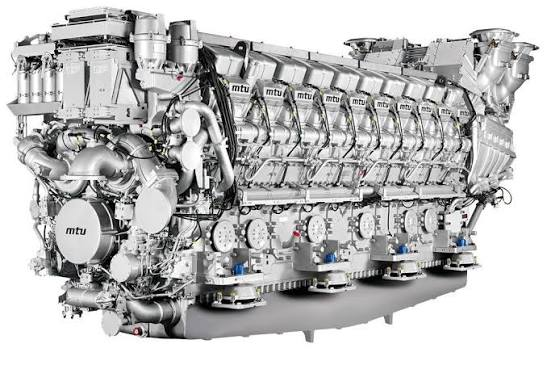
\includegraphics[width=0.5\linewidth]{CHAPTER 2/MTU 20V 8000 M71.png}
    \caption{MTU 20V 8000 M71 \cite{maritimeprofessional2012mtu8000}}
    \label{fig:placeholder}
\end{figure}
\subsection{Selection of Gas Turbine}For high-speed operation, a GE LM2500 marine gas turbine was selected. The LM2500 is a well-established marine gas turbine and has extensive experience in naval propulsion applications. The LM2500 has an output of approximately 22.07 MW under U.S. Navy Standard Day conditions. This rating was considered for the present preliminary design because it represents a suitable naval operating reference condition. The gas turbine provides a large increase in available propulsion power when high speed is required. Therefore, it is used in conjunction with diesel engines during high-speed operation.
\begin{figure}[htbp]
    \centering
    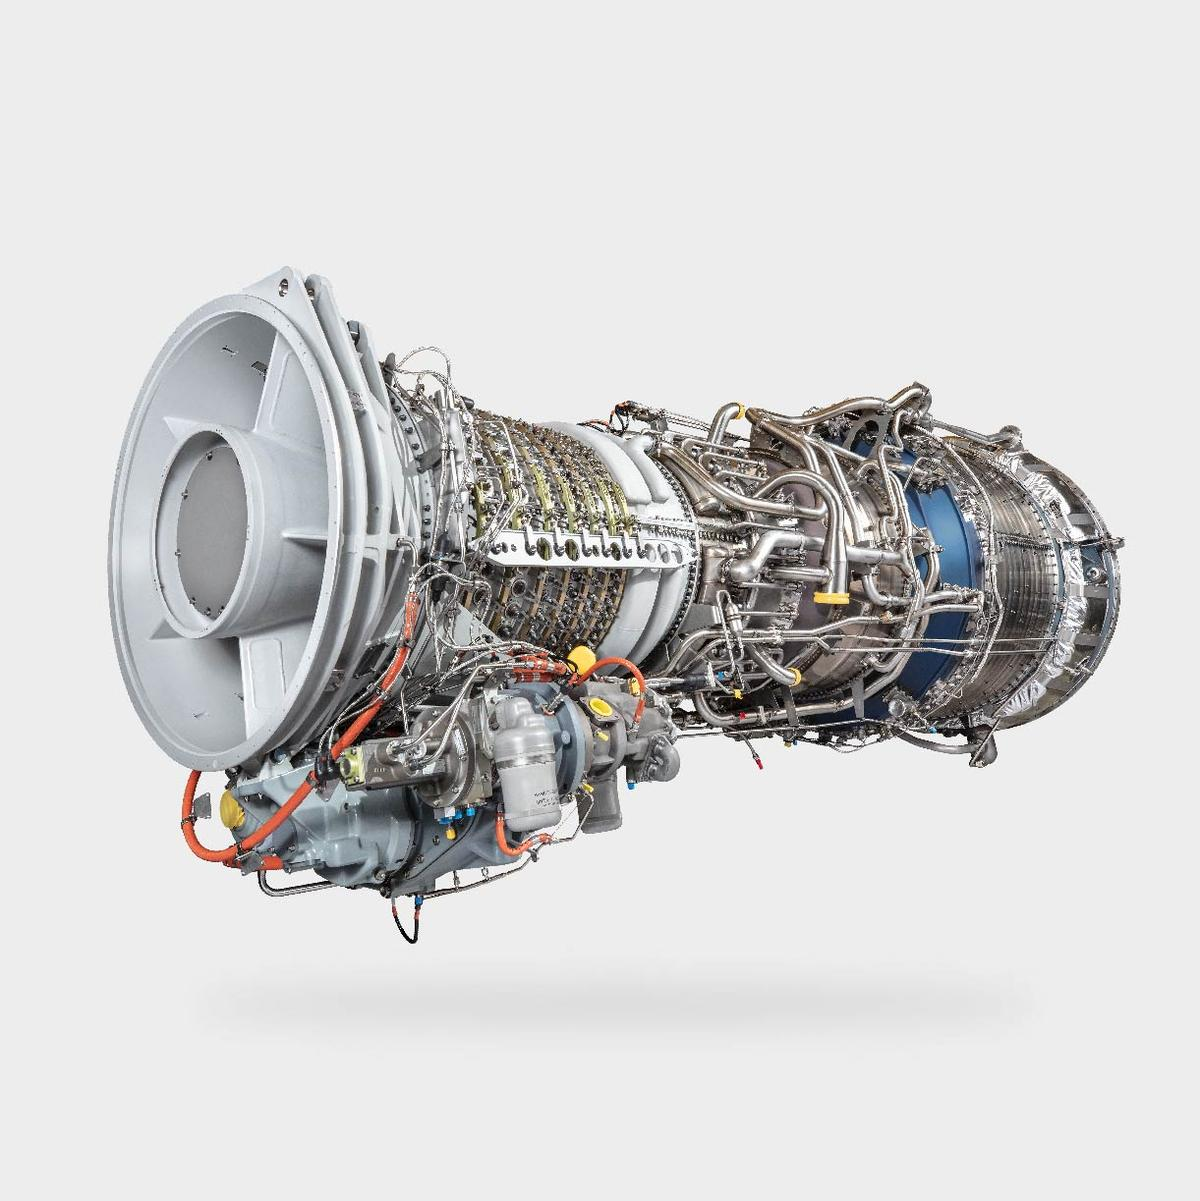
\includegraphics[width=0.4\linewidth]{CHAPTER 2/GE LM2500 marine gas turbine.png}
    \caption{GE LM2500 marine gas turbine \cite{thehindu2024lm2500}}
    \label{fig:placeholder}
\end{figure}
\subsection{Preliminary Machinery selection}
\begin{table}[htbp]
    \centering
    \caption{Preliminary Machinery Selection}
    \label{tab:preliminary_machinery_selection}

    \footnotesize
    \setlength{\tabcolsep}{5pt}

    \begin{tabular}{llcccc}
        \toprule
        \textbf{System} &
        \textbf{Machinery} &
        \textbf{Qty.} &
        \textbf{Power/unit} &
        \textbf{Total} \\
        \midrule

        Main propulsion &
        MTU 20V 8000 M71 diesel \cite{mtu_20v8000_m71} &
        2 &
        8.20 MW &
        16.40 MW \\

        Main propulsion &
        GE LM2500 gas turbine \cite{ge_lm2500} &
        1 &
        22.07 MW &
        22.07 MW \\

        \textbf{Propulsion total} &
        &
        &
        &
        \textbf{38.47 MW} \\

        Electrical generation &
        Caterpillar 3512C genset \cite{caterpillar_3512c} &
        3 &
        1.70 MW &
        5.10 MW \\

        \bottomrule
    \end{tabular}

    \vspace{2mm}
    \footnotesize
    \textit{Note: The propulsion plant consists of two diesel engines and one gas turbine in a CODAG configuration.}
\end{table}
\noindent A CODAG (Combined Diesel and Gas Turbine) propulsion configuration
consisting of two diesel engines and one gas turbine was selected for
the proposed vessel. The use of a single gas turbine is a proven
arrangement in naval vessels. For example, the German Navy's
F124 Sachsen-class frigates
\cite{f124_sachsen_bundeswehr,ge_marine_frigate_propulsion}
employ a CODAG propulsion system consisting of two diesel engines
and one gas turbine, with a total installed propulsion power of
approximately 38.3~MW and a maximum speed of about 29~kn.

\vspace{\baselineskip}\par\noindent The proposed propulsion plant consists of two MTU 20V 8000 M71
diesel engines, each rated 8.20~MW, and one GE LM2500 gas turbine
rated 22.07~MW. The total installed propulsion power resulting is :

\[
P_{\mathrm{total}}
=
2(8.20) + 22.07
=
38.47~\mathrm{MW}.
\]
\section{Preliminary General Arrangement}
A preliminary general arrangement (GA) of a ship is an early-stage layout plan showing the main arrangement of spaces, equipment, and systems throughout the vessel. Typically, it identifies the hull divisions, decks, accommodation, machinery spaces, cargo areas, tanks, access routes, safety equipment, and major shipboard facilities. This drawing is used to assess whether the functions, capacity, stability, safety, and operational requirements of the ship can be met before the detailed design begins.
\subsection{Positions of Frames}According to the Indian Register of Shipping (IRS) Rules. The reference spacing is based on the length of run (LR), calculated using the adopted Taylor’s expression.
\begin{equation}
LR = 0.2L_{WL} + 2.5(B \times T)^{0.5}
\label{eq : 2.3}
\end{equation}

\[
LR = 0.2(113) + 2.5(15.04 \times 5.3)^{0.5}
\]
From (\ref{eq : 2.3})
\[
LR = 44.92~\mathrm{m}
\]

The reference spacing for the longitudinal framing is calculated using
the IRS formula.

\begin{equation}
S_r = 550 + 2 \times LR \quad (\mathrm{mm})
\label{eq : 2.4}
\end{equation}

\[
S_r = 550 + 2(44.92)
\]
From (\ref{eq : 2.4})
\[
S_r = 639.84~\mathrm{mm}
\]

Therefore, the reference spacing for the longitudinal framing is
approximately $640~\mathrm{mm}$.
$$S_r=640mm$$
The calculation of reference spacing is subject to regional maximum limits prescribed by IRS Rules. The governing frame spacing for each region is obtained by adopting the lesser of the calculated spacing and the applicable IRS limits.

\begin{table}[htbp]
    \centering
    \caption{IRS Regional Limits and Adopted Frame Spacing}
    \label{tab:irs_frame_spacing}

    \small
    \setlength{\tabcolsep}{4pt}

    \begin{tabular}{lccc}
        \toprule
        \textbf{Ship Region} &
        \textbf{IRS Limit (mm)} &
        \textbf{Calculated (mm)} &
        \textbf{Adopted (mm)} \\
        \midrule

        Peaks and cruiser stern & 600  & 640 & 600 \\
        Forward region         & 700  & 640 & 650 \\
        Midship region         & 1000 & 640 & 650 \\

        \bottomrule
    \end{tabular}
\end{table}
\subsubsection{Location of Collision Bulkhead}

The location of the collision bulkhead is calculated in accordance
with IRS rules.

\noindent For ships with $LR < 200$~m, the IRS limits are:

\begin{equation}
X_{c,\min} = 0.05LR - X_R
\label{eq : 2.5}
\end{equation}

\begin{equation}
X_{c,\max} = 0.08LR - X_R
\label{eq : 2.6}
\end{equation}

\noindent where $X_R$ is the correction factor that accounts for underwater
projections from FP.

\noindent The correction factor is calculated as:

\begin{equation}
X_R = 0.015LR
\label{eq : 2.7}
\end{equation}

\noindent For the proposed vessel:

\[
X_R = 0.67~\mathrm{m}
\]

\noindent Therefore from (\ref{eq : 2.5}) \& (\ref{eq : 2.6}),

\[
X_{c,\min} = 1.576~\mathrm{m}
\]

\[
X_{c,\max} = 2.92~\mathrm{m}
\]

\noindent Based on the above limits, the collision bulkhead is selected at
$2.248$~m from the forward perpendicular (FP) point.\subsection{Height of Superstructure}The height of the superstructure depends on the required Blind region, according to SOLAS Regulation 22, the blind region should not be more than twice the length of the vessel or 500 m, whichever is lesser. \vspace{\baselineskip} \par\noindent Considering the blind region as 2 times the ship length, which is 232 m and height of human as 1.53 m.
\begin{figure}[htbp]
    \centering
    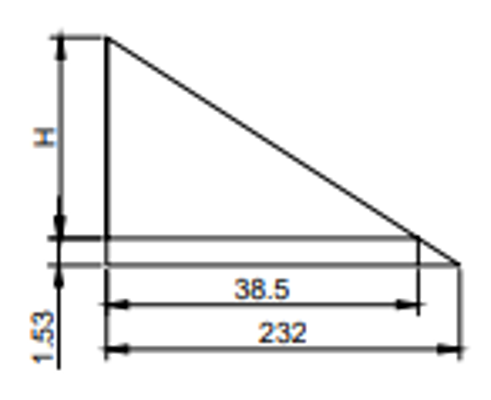
\includegraphics[width=0.5\linewidth]{CHAPTER 2/superstructure.png}
    \caption{Superstructure height}
    \label{fig:placeholder}
\end{figure}
From the above figure it was found that the minimum superstructure height should be 0.217 m. However, we take the height of the superstructure to be 9m.
\vspace{\baselineskip}\par\noindent With these calculations, a preliminary general arrangement drawing was developed.
\begin{figure}[htbp]
    \centering
    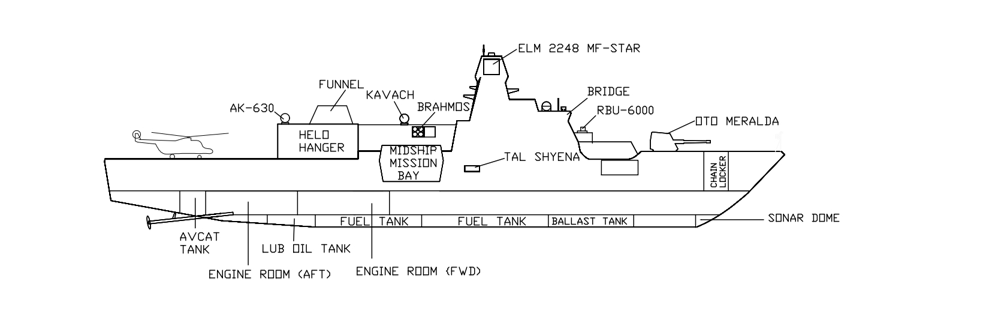
\includegraphics[width=\textwidth]{CHAPTER 2/side view.png}
    \caption{Preliminary General Arrangement}
    \label{fig:preliminary_general_arrangement}
\end{figure}
\section{Initial Estimation of Consumable Stores and Cargoes}

This part deals with the estimation of requirements such as fuel,
lube oil, provisions, fresh water, cargo, etc. It also influences the
weight estimation stage during the design.

\subsection{Mass of HFO (\texorpdfstring{$M_{\mathrm{HFO}}$}{MHFO})}

Since the vessel requires an endurance of 30 days to support all
operations specified in OSR, the mass of heavy fuel oil is calculated
as:

\begin{equation}
M_{\mathrm{HFO}}
=
\frac{\mathrm{SFC}\;(\mathrm{g/kWh}) \times P_B\;(\mathrm{kW})
\times \mathrm{hours}}{1{,}000{,}000}
\times 1.10
\end{equation}

\[
M_{\mathrm{HFO}} = 453~\text{tonnes}
\]
\subsection{Mass of Diesel Fuel}

The mass of diesel fuel is estimated as

\begin{equation}
M_{\mathrm{DF}} = \frac{M_{\mathrm{HFO}}}{3}
\end{equation}

\[
M_{\mathrm{DF}} = 151~\text{tonnes}
\]


\subsection{Mass of Lube Oil}

The mass of lube oil is estimated as:

\begin{equation}
M_{\mathrm{LO}}
=
0.04\left(M_{\mathrm{HFO}} + M_{\mathrm{DF}}\right)
\end{equation}

\[
M_{\mathrm{LO}} = 24.16~\text{tonnes}
\]


\subsection{Mass of Fresh Water (\texorpdfstring{$M_{\mathrm{FW}}$}{MFW})}

This will include the mass of drinking water and washing water.
The vessel has a complement of 138 persons.

\vspace{\baselineskip}\par\noindent The drinking water requirement is 10 liters/person / day and
the washing water is 80 liters / person / day. Considering that the vessel
operates continuously for 30 days:

\[
\text{Weight of drinking water}
=
\frac{(138 \times 10)\times 30}{1000}
\times 1.10
\]

\[
= 45.54~\text{tonnes}
\]

\vspace{\baselineskip}\par\noindent The weight of washing water is:

\[
\text{Weight of washing water}
=
\frac{(138 \times 80)\times 30}{1000}
\times 1.10
\]

\[
= 365~\text{tonnes}
\]

\vspace{\baselineskip}\par\noindent Hence, the total fresh water requirement is:

\[
M_{\mathrm{FW}}
=
45.54 + 365
=
410~\text{tonnes}
\]


\subsection{Mass of Ballast Water (\texorpdfstring{$M_{\mathrm{BW}}$}{MBW})}

The ballast water allowance is generally taken as 2--3\% of the
full-load displacement. Taking into account 2.5\% of $\Delta = 3600$~t:

\[
M_{\mathrm{BW}}
=
0.025 \times 3600
\]

\[
M_{\mathrm{BW}} = 90~\text{tonnes}
\]


\subsection{Mass of Provisions (\texorpdfstring{$M_{\mathrm{PR}}$}{MPR})}

Taking into account the provisions requirement as 8~kg / person/day, including
factors such as delays in the journey and food spoilage, for a crew
of 138 persons over an endurance period of 30 days, the mass of
provisions is calculated as follows:

\begin{equation}
M_{\mathrm{PR}}
=
\frac{N_{\mathrm{crew}} \times 8 \times 30}{1000}
\times 1.10
\end{equation}

\[
M_{\mathrm{PR}} = 37~\text{tonnes}
\]


\section{Checks on Tank Capacity}

The total underwater volume up to the main deck is calculated as:

\begin{equation}
V_{\mathrm{md}}
=
L_{WL} B T C_B
\left(\frac{D}{T}\right)^{C_W/C_B}
\end{equation}

\[
V_{\mathrm{md}} = 10126.98~\mathrm{m^3}
\]

\vspace{\baselineskip}\par\noindent According to the IRS Naval Rules, Section 7.1.3, a double bottom
is generally to be provided as far as practicable and compatible with
the design and proper working of the ship to the extent determined by
the Naval Authority. The double bottom may be omitted in watertight
compartments used exclusively for the carriage of liquids.

\vspace{\baselineskip} \par \noindent Furthermore, as per Clause 7.3.1.1, the minimum depth of the center girder is 
given by:
\begin{equation}
d = 250 + 20B + 50T \quad [\mathrm{mm}]
\end{equation}

\[
d = 835~\mathrm{mm}
\]

\vspace{\baselineskip} \par \noindent Therefore, the double bottom height is taken as $1~\mathrm{m}$.

\section{Preliminary Resistance and Propulsion Performance}

\subsection{Resistance Calculation by Guldhammer--Harvald Method}

The total resistance is given by:

\begin{equation}
R_T = C_T \times \frac{1}{2}\rho S V^2
\label{eq : 2.14}
\end{equation}

\vspace{\baselineskip} \par \noindent where

\begin{equation}
C_T = C_F + C_R + C_A + C_{AA}
\label{eq : 2.15}
\end{equation}

\vspace{\baselineskip} \par \noindent where:
\begin{itemize}
    \item $C_F$ = coefficient of friction resistance,
    \item $C_R$ = residual resistance coefficient,
    \item $S$ = wet surface area,
    \item $V$ = vessel speed,
    \item $C_A$ = correlation allowance,
    \item $C_{AA}$ = model--ship correlation allowance.
\end{itemize}

\vspace{\baselineskip} \par \noindent The waterline length is

\[
L_{WL} = 113~\mathrm{m}
\]

\vspace{\baselineskip} \par \noindent The coefficient of friction resistance is calculated using the following:

\begin{equation}
C_F =
\frac{0.075}{(\log_{10}Re-2)^2}
\end{equation}


\vspace{\baselineskip} \par \noindent The residual resistance coefficient, $C_R$, is obtained from the
graph $L_{WL}/\nabla^{1/3}$ shown in Figures \ref{fig:Residuary resistance coefficicent for 7} and \ref{fig:Residuary resistance coefficicent for 7.5}.

\[
\frac{L_{WL}}{\nabla^{1/3}} = 7.39
\]

\vspace{\baselineskip} \par \noindent The value of $C_R$ is obtained by interpolation between the values
corresponding to 7 and 7.5 to obtain the value for 7.39.

\[
C_P = 0.68
\]\begin{figure}[htbp]
    \centering
    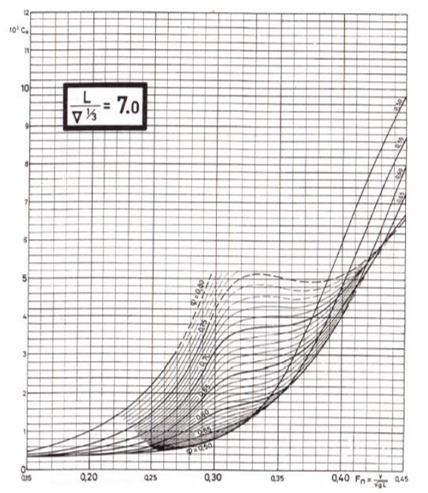
\includegraphics[width=0.5\linewidth]{CHAPTER 2/Residuary resistance coefficicent for 7.png}
    \caption{Residuary resistance coefficicent for 7 \cite{itu_gem341e_hydrodynamics} }
    \label{fig:Residuary resistance coefficicent for 7}
\end{figure}
\begin{figure}[htbp]
    \centering
    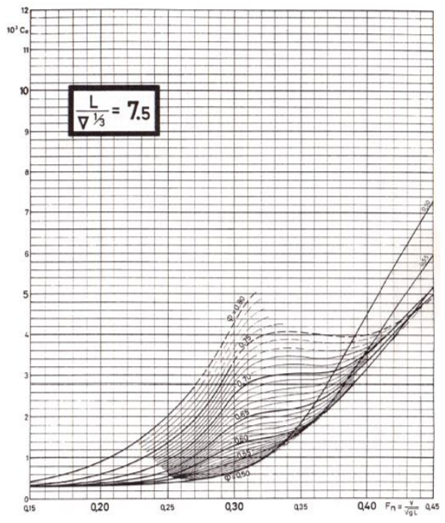
\includegraphics[width=0.5\linewidth]{CHAPTER 2/Residuary resistance coefficicent for 7.5.png}
    \caption{Residuary resistance coefficicent for 7.5 \cite{itu_gem341e_hydrodynamics}}
    \label{fig:Residuary resistance coefficicent for 7.5}
\end{figure}
\vspace{\baselineskip} \par \noindent Resistance and effective power were evaluated at the design
cruising speed of 15 knots. A separate resistance prediction was
 performed at the maximum speed of 28 knots to assess the propulsion
power requirement under the maximum operating conditions.

\subsection{B/T Correction}

The Guldhammer--Harvald resistance diagrams are based on a standard
width-to-draft ratio of $B/T=2.5$. Therefore, a correction is applied
to the actual breadth-to-draft ratio of the vessel
\cite{itu_gem341e_hydrodynamics}.

\vspace{\baselineskip} \par \noindent The correction is calculated as follows:

\begin{equation}
10^3\Delta C_R =
0.16\left(\frac{B}{T}_{\mathrm{design}}-2.5\right)
\cite{itu_gem341e_hydrodynamics}
\end{equation}

\subsection{Section Correction}

Since the shape of the forebody and the afterbody is considered normal,
no section correction is applied
\cite{itu_gem341e_hydrodynamics}.

\subsection{Appendage Correction}

The effects of standard appendages, such as the rudder and bilge keels
, are already included in the residual resistance coefficient, $C_R$.
An additional appendage resistance allowance is considered for the
boasting and a $5\%$ allowance for shaft brackets and shafts
\cite{itu_gem341e_hydrodynamics}.

\subsection{Additional Resistance Components}

The additional resistance components considered in the calculation
are the air resistance and the steering resistance.

\vspace{\baselineskip} \par \noindent The air resistance coefficient is taken as:

\[
10^3 C_{AA}=0.07
\cite{itu_gem341e_hydrodynamics}
\]

\vspace{\baselineskip} \par \noindent The steering resistance coefficient is taken as:

\[
10^3 C_{AS}=0.04 \cite{itu_gem341e_hydrodynamics}
\]

\vspace{\baselineskip} \par \noindent From (\ref{eq : 2.15}) The total resistance coefficient is calculated as:

\[
C_T=C_F+C_R+C_{AA}+C_{AS}
\cite{itu_gem341e_hydrodynamics}
\]

\vspace{\baselineskip} \par \noindent The total resistance is then calculated from (\ref{eq : 2.14}) :

\[
R_T=C_T\left(\frac{1}{2}\rho S V^2\right)
\cite{itu_gem341e_hydrodynamics}
\]

\vspace{\baselineskip} \par \noindent where $C_T$ is the total resistance coefficient, $\rho$ is the
density of water, $S$ is the wet surface area and $V$ is the
 speed of the vessel.

\vspace{\baselineskip} \par \noindent The wetted surface area is estimated using the following:

\begin{equation}
S=0.99\left(\frac{\nabla}{T}+1.9L_{WL}T\right)
+A_{\mathrm{tunnel}}
\cite{itu_gem341e_hydrodynamics}
\end{equation}

\vspace{\baselineskip} \par \noindent where $\nabla$ is the displacement volume, $T$ is the draft,
$L_{WL}$ is the length of the waterline and $A_{\mathrm{tunnel}}$ is the
surface area associated with the tunnel.

\vspace{\baselineskip} \par \noindent For the initial calculations, $A_{\mathrm{tunnel}}$ is taken as the
cross-sectional area of a cylinder.
\subsection{Calculation of QPC}

The Quasi-Propulsive Coefficient (QPC) is a measure of the overall
effectiveness of converting the power delivered to the propeller into
the useful power required to move the ship forward
\cite{itu_gem341e_hydrodynamics}.

\vspace{\baselineskip} \par \noindent The quasi-propulsive coefficient is calculated as:

\begin{equation}
QPC =
3.6C_B
\left(1-0.9C_B\right)
-
\frac{V_{MS}}{4.8C_B\sqrt{L}}
\cite{itu_gem341e_hydrodynamics}
\end{equation}

\subsection{Powering Calculation}

The effective power required to overcome the total resistance is
calculated as:

\begin{equation}
P_E=R_TV
\cite{itu_gem341e_hydrodynamics}
\end{equation}

\vspace{\baselineskip} \par \noindent where $P_E$ is the effective power, $R_T$ is the total resistance 
and $V$ is the speed of the ship.

\vspace{\baselineskip} \par \noindent The delivered power is given by:

\begin{equation}
P_D=\frac{P_E}{QPC}
\cite{itu_gem341e_hydrodynamics}
\end{equation}

\vspace{\baselineskip} \par \noindent Since a diesel-electric (DE) propulsion system is used, the propulsion
efficiency is taken as:

\[
\eta=0.9
\]

\vspace{\baselineskip} \par \noindent The required brake power is therefore calculated by applying a $15\%$
margin:

\begin{equation}
P_B=\frac{P_D}{\eta}\times1.15
\cite{itu_gem341e_hydrodynamics}
\end{equation}


\begin{table}[H]
    \centering
    \caption{Resistance Calculation at Cruising and Maximum Speeds}
    \label{tab:resistance_calculation}

    \normalsize
    \setlength{\tabcolsep}{12pt}
    \renewcommand{\arraystretch}{1.25}

    \begin{tabular}{lcc}
        \toprule
        \textbf{Parameter} & \textbf{28 knots} & \textbf{15 knots} \\
        \midrule
        Reynolds Number        & 1379294892 & 985206779.7 \\
        Frictional Coefficient & 0.00147132 & 0.001533447 \\
    
        Froude Number          & 0.432      & 0.308 \\
        $C_R$ & 7.439738029 & 2.910181213 \\

        B/T Correction         & 0.083      & 0.083 \\
        Roughness              & 0.2        & 0.2 \\
        Air                    & 0.07       & 0.07 \\
        Steering               & 0.04       & 0.04 \\
        Residual Coefficient   & 0.00842    & 0.00353 \\
        
        Total Coefficient      & 0.0098     & 0.0050 \\
        Wetted Surface Area    & 1825~m$^2$ & 1825~m$^2$ \\
        Total Resistance       & 1912~kN & 978.8~kN \\
        QPC                    & 0.211      & 0.412 \\
        Power                  & 27.53~MW   & 14.098~MW \\
        \bottomrule
    \end{tabular}

    \vspace{3mm}

    \footnotesize
    \textit{Source: Author's calculation based on the methods given in
    \cite{itu_gem341e_hydrodynamics}.}
\end{table}
\section{Initial Trim and Stability Calculations}

In this section, the initial trim, stability, and freeboard of the
vessel are calculated on the basis of the values derived from the previous
sections.

\subsection{Stability Calculations}

The preliminary stability of the vessel is evaluated using the
 principal dimensions and the available hull form parameters. The
calculation is based on the characteristics of the proposed vessel
and the corresponding stability methodology
% \cite{goren_ship_hydrodynamics_resistance}. % Citation key not found in refernce.bib

\vspace{\baselineskip} \par \noindent The principal dimensions considered for the preliminary calculations
are the following:

\[
\begin{aligned}
L &= 116~\mathrm{m} \\
B &= 16~\mathrm{m} \\
T &= 5.434~\mathrm{m} \\
D &= 10~\mathrm{m}
\end{aligned}
\]
\vspace{\baselineskip} \par \noindent The principal ratios of the vessel are calculated as:

\[
\frac{L}{B}=7.25
\]

\[
\frac{B}{T}=2.994
\]

\[
\frac{D}{T}=1.84
\]

\vspace{\baselineskip} \par \noindent The righting lever, $GZ$, is calculated using the following
relationship:

\begin{equation}
GZ = GM\sin(\theta)+BM\times h^*
\end{equation}

\vspace{\baselineskip} \par \noindent where $\theta$ is the angle of heel and $h^*$ is the constant obtained
from Prohaska's curve (CRS).

\vspace{\baselineskip} \par \noindent Here,

\begin{itemize}
    \item $\theta$ = angle of heel,
    \item $h^*$ = constant obtained from Prohaska's curve (CRS),
    \item $BM$ = metacentric radius,
    \item $GM$ = metacentric height.
\end{itemize}

\vspace{\baselineskip} \par \noindent The metacentric height is calculated as:

\begin{equation}
GM = KB + BM - KG
\end{equation}

\vspace{\baselineskip} \par \noindent where

\begin{equation}
KB=
\left[
\frac{C_W}{C_W+C_B}
\right]T
\label{eq : 2.25}
\end{equation}

\vspace{\baselineskip} \par \noindent For the present vessel,

\[
C_W=6
\]

\vspace{\baselineskip} \par \noindent Therefore,

\[
KB=
\left[
\frac{6}{6+0.4}
\right]\times5
=3.036~\mathrm{m}
\]

\vspace{\baselineskip} \par \noindent The metacentric radius is given by:

\begin{equation}
BM=\frac{C_{IT}B^2}{12T}
\label{eq : 2.26}
\end{equation}

\vspace{\baselineskip} \par \noindent where $C_{IT}$ is a factor based on the shape of the waterplane.

\vspace{\baselineskip} \par \noindent According to Normand:

\begin{equation}
C_{IT}=0.894C_W^2+0.096 \cite{prohaska_paper_1262}
\end{equation}

\vspace{\baselineskip} \par \noindent Therefore,

\[
C_{IT}=0.894(0.6)^2+0.096=0.4
\]

\vspace{\baselineskip} \par \noindent According to Dankwart:

\begin{equation}
C_{IT}=0.87C_W^2+0.13C_W
\end{equation}

\vspace{\baselineskip} \par \noindent Therefore,

\[
C_{IT}=0.87(0.6)^2+0.13(0.6)=0.38
\]

\vspace{\baselineskip} \par \noindent Hence, from (\ref{eq : 2.26}) the metacentric radius is:

\[
BM=4.025~\mathrm{m}
\]

\vspace{\baselineskip} \par \noindent Taking the vertical centre of gravity as:

\[
KG=5.7~\mathrm{m}
\]

\vspace{\baselineskip} \par \noindent from (\ref{eq : 2.25}) the calculated value of $KB$ as:

\[
KB=3.188~\mathrm{m}
\]

\vspace{\baselineskip} \par \noindent the metacentric height is:

\[
GM=KB+BM-KG
\]

\[
GM=3.188+4.025-5.7
\]

\[
GM=1.514~\mathrm{m}
\]

\vspace{\baselineskip} \par \noindent The residual stability arm, $h^*$, can then be determined for each
angle of heel using Prohaska's curves.
\begin{table}[H]
    \centering
    \caption{GZ Values}
    \label{tab:gz_values}
    \small
    \setlength{\tabcolsep}{7pt}
    \renewcommand{\arraystretch}{1.2}

    \begin{tabular}{ccccccc}
        \toprule
        \textbf{S.No} &
        \textbf{Heel Angle} &
        \textbf{$\sin\theta$} &
        \textbf{$GM\sin\theta$} &
        \textbf{$C_{RS}$} &
        \textbf{$BM C_{RS}$} &
        \textbf{$GZ$} \\
        \midrule
        1 & 0  & 0    & 0        & 0         & 0        & 0 \\
        2 & 15 & 0.25 & 0.391869 & 3.2E-05   & 0.000129 & 0.391998 \\
        3 & 30 & 0.5  & 0.757032 & -0.02041  & -0.08216  & 0.674871 \\
        4 & 45 & 0.707& 1.070605 & -0.0833   & -0.33528  & 0.735326 \\
        5 & 60 & 0.86 & 1.311219 & -0.14858  & -0.59806  & 0.713161 \\
        6 & 75 & 0.96 & 1.462474 & -0.26776  & -1.07778  & 0.384698 \\
        7 & 90 & 1    & 1.514065 & -0.3425   & -1.37862  & 0.135448 \\
        \bottomrule
    \end{tabular}

    \vspace{2mm}
    \footnotesize
    \textit{Source: Author's calculation based on Prohaska's curves
    \cite{prohaska_paper_1262}.}
\end{table}
\begin{figure}
    \centering
    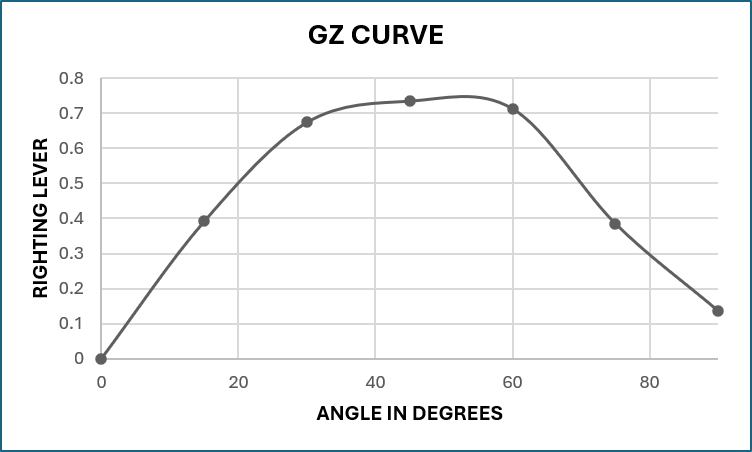
\includegraphics[width=01\linewidth]{CHAPTER 2/GZ CURVE.png}
    \caption{gz curve}
    \label{fig:placeholder}
\end{figure}
\vspace{\baselineskip} \par \noindent From the GZ curve, the following values were obtained:

\begin{enumerate}[\alph*)]
    \item Area up to $30^\circ = 0.19573$
    
    \item Area up to $40^\circ = 0.71517$
    
    \item Area between $30^\circ$ and $40^\circ = 0.51945$
    
    \item Righting lever ($GZ$) at an angle of $30^\circ = 0.67487~\mathrm{m}$
    
    \item The angle of maximum righting lever is $50^\circ$
    
    \item Initial metacentric height is $1.51406~\mathrm{m}$
\end{enumerate}

\vspace{\baselineskip} \par \noindent Since the GZ curve satisfies all the specified stability criteria, the
initial stability of the vessel is therefore verified.

\subsection{Initial Trim Checks}

Stability checks have been verified by plotting the GZ
curve. Although initial trim checks would typically follow, they require
detailed General Arrangement and capacity metrics that are not yet
established. As the current project scope is focused on finalizing the
main dimensions, trim calculations have been postponed to later
design stages.
\section{Initial Freeboard Calculations}

The freeboard is the vertical distance between the lower waterline and
the upper surface of the freeboard deck measured on the side along
the draft markings. The freeboard deck is defined as the uppermost
continuous deck having permanent means of closing all openings in
the weather-exposed portions of the deck and sides of the ship.

\vspace{\baselineskip} \par \noindent The freeboard calculation is carried out in accordance with the
International Convention on Load Lines, 1966 (ICLL 1966)
\cite{international_load_lines_1966}.
\subsection{Tabular Freeboard}

Vessels as per the International Convention on Load Lines, 1966
(ICLL 1966) are divided into two major categories:

\begin{enumerate}[\alph*)]
    \item \textbf{Type ``A'':} A ship which is designed to carry only
    liquid cargoes in bulk, and in which cargo tanks have only small
    access openings closed by watertight gasketed covers of steel or
    equivalent material.

    \item \textbf{Type ``B'':} All ships which do not come within the
    provisions regarding Type ``A'' ships in paragraphs (2) and (3)
    of the relevant regulation shall be considered as Type ``B'' ships.
\end{enumerate}

\vspace{\baselineskip} \par \noindent Therefore, the proposed vessel falls under \textbf{Type ``B''}. According to
the loading line convention, the minimum tabular freeboard for a ship of
length $116~\mathrm{m}$ is $1609~\mathrm{mm}$. Corrections are applied
to this tabular freeboard as described below.

\begin{enumerate}[\alph*)]

    \item \textbf{Correction for $C_B$}

    If $C_B > 0.68$, a correction is required. Since the block
    coefficient of the proposed vessel is

    \[
    C_B = 0.38 < 0.68,
    \]

    no correction is applied to the tabular freeboard.

    \item \textbf{Correction for Depth}

    If

    \[
    \frac{L}{15} < D,
    \]

    \vspace{\baselineskip} \par \noindent a correction for depth is required. For the proposed vessel,

    \[
    \frac{L}{15}
    = \frac{116}{15}
    = 7.7333~\mathrm{m},
    \]

    which is less than the design depth of $10~\mathrm{m}$.
    Therefore, the depth correction is applied.

    The correction is calculated as

    \begin{equation}
    \text{Correction}
    =
    \left(D-\frac{L}{15}\right)R
    \label{eq : 2.29}
    \end{equation}

    where $R$ is the correction rate.

    For the proposed vessel,

    \[
    R = 241.667~\mathrm{mm}
    \]

    and therefore from (\ref{eq : 2.29}),

    \[
    \begin{aligned}
    \text{Correction}
    &=
    \left(10-\frac{116}{15}\right)(241.667)\\
    &= 547.7778~\mathrm{mm}.
    \end{aligned}
    \]

    \item \textbf{Correction for Superstructure}

    Type ``B'' ships are classified into two types depending on the
    presence of a detached bridge. The proposed vessel is classified
    as a Type ``B'' ship without a detached bridge.

    The effective length of the superstructure is

    \[
    L_E = 65.363~\mathrm{m},
    \]

    which corresponds to

    \[
    \frac{65.363}{116}\times100
    = 56.34\%
    \]

    of the length of the vessel. As per the Load Line Convention,
    the corresponding reduction in freeboard is given in the
    following table.


\begin{table}[htbp]
    \centering
    \caption{Percentage of Deduction for Type ``B'' Ships}
    \label{tab:freeboard_deduction_type_b}
    
    \resizebox{\textwidth}{!}{%
    \begin{tabular}{llccccccccccc}
        \toprule
        \textbf{Ships} & \textbf{Line}
        & \textbf{0} & \textbf{0.1L} & \textbf{0.2L} & \textbf{0.3L}
        & \textbf{0.4L} & \textbf{0.5L} & \textbf{0.6L}
        & \textbf{0.7L} & \textbf{0.8L} & \textbf{0.9L} & \textbf{1.0L} \\
        \midrule
        
        Ships with forecastle and without detached bridge
        & I
        & 0 & 5 & 10 & 15 & 23.5 & 32 & 46 & 63 & 75.3 & 87.7 & 100 \\
        
        Ships with forecastle and detached bridge
        & II
        & 0 & 6.3 & 12.7 & 19 & 27.5 & 36 & 46 & 63 & 75.3 & 87.7 & 100 \\
        
        \bottomrule
    \end{tabular}%
    }
    
    \vspace{2mm}
    
    \footnotesize
    \textit{Source: International Convention on Load Lines, 1966,
    Regulation 37 \cite{international_load_lines_1966}.}
\end{table}
From interpolation, it was found that for an effective superstructure
length of $56.34\%$ of $L$, the corresponding deduction in freeboard is
$40.886\%$.

Therefore, the correction in freeboard is

\[
\begin{aligned}
\text{Correction}
&= -0.40886 \times 1609\\
&= -657.862~\mathrm{mm}.
\end{aligned}
\]

\item \textbf{Correction for Sheer}

The proposed vessel has no sheer. Hence, a correction is applied for
sheer deficiency. This correction results in an increase in the
freeboard.

The correction for sheer shall be the deficiency or excess of sheer
(see paragraphs (9) to (11) inclusive of Regulation 38), multiplied
by

\begin{equation}
0.75-\frac{S}{2L} \cite{international_load_lines_1966}
\label{eq : 2.30}
\end{equation}

where $S$ is the total length of enclosed superstructures.

The sheer deficiency is calculated as per the table given below:
\begin{table}[H]
    \centering
    \caption{Sheer Deficiency}
    \label{tab:sheer_deficiency}

    \scriptsize
    \setlength{\tabcolsep}{6pt}
    \renewcommand{\arraystretch}{1.15}

    % ---------------- Forward Half ----------------
    \begin{tabular}{l l c c}
        \toprule
        \textbf{Section} &
        \textbf{Station} &
        \textbf{Ordinate (in mm)} &
        \textbf{Factor} \\
        \midrule

        \textbf{Forward half}
        & Amidships
        & 0
        & 1 \\

        & 1/3 L from F.P.
        & $5.6(L/3+10)$
        & 3 \\

        & 1/6 L from F.P.
        & $22.2(L/3+10)$
        & 3 \\

        & Forward Perpendicular
        & $50(L/3+10)$
        & 1 \\

        \midrule

        % ---------------- After Half ----------------
        \textbf{After half}
        & After Perpendicular
        & $25(L/3+10)$
        & 1 \\

        & 1/6 L from A.P.
        & $11.1(L/3+10)$
        & 3 \\

        & 1/3 L from A.P.
        & $2.8(L/3+10)$
        & 3 \\

        & Amidships
        & 0
        & 1 \\

        \bottomrule
    \end{tabular}

    \vspace{2mm}

    {\footnotesize
    \textit{Source: International Convention on Load Lines, 1966,
    Regulation 38 \cite{international_load_lines_1966}.}
    }

\end{table}
\[
\text{Sheer Deficiency}
=
(4.168L+125.06)
=
608.548~\mathrm{mm}
\]

The correction for sheer is therefore followed from (\ref{eq : 2.30}) as,

\[
\begin{aligned}
\text{Correction}
&=
\left(0.75-0.281\right)(608.548)\\
&=
284.9605~\mathrm{mm}.
\end{aligned}
\]
\end{enumerate}
\vspace{\baselineskip} \par \noindent Hence, the final freeboard is 1783.877 mm. This is much smaller than the 4.7 m design freeboard, and therefore the freeboard criteria are satisfied.
\clearpage
\section{Conclusion}

The final main dimensions of the vessel have been frozen after
iterative checks of hydrostatics, stability, and resistance-powering
balance. The selected length of $116~\mathrm{m}$ provides sufficient
deck area for aviation and ASW operations, while maintaining
favorable slenderness ratios ($L/B \approx 7.25$, $L/T \approx 21.8$)
to ensure good course-keeping and maneuverability in littoral waters.
The breadth of $16~\mathrm{m}$ has been chosen to enhance stability
and provide a broad wet-deck volume, while also producing a relatively
shallow block ratio ($T/B = 0.331$) that contributes to improved
turning ability. The depth of $10~\mathrm{m}$ offers significant
reserve buoyancy and freeboard, with the actual freeboard
($4.7~\mathrm{m}$) exceeding the ICLL requirements by a large margin,
ensuring compliance with safety standards. The design draft of
$5.3~\mathrm{m}$ is kept shallow to allow operations close to shore,
while maintaining an adequate displacement of approximately
$3650~\mathrm{t}$ to house payload, vehicles, and aviation
facilities.

\begin{table}[htbp]
    \centering
    \caption{Main Particulars of the Ship}
    \label{tab:main_particulars}
    \small
    \setlength{\tabcolsep}{12pt}
    \renewcommand{\arraystretch}{1.2}
    
    \begin{tabular}{lc}
        \toprule
        \textbf{Parameter} & \textbf{Value} \\
        \midrule
        LOA          & 116 m \\
        B            & 16 m \\
        $L_{WL}$     & 113 m \\
        $B_{WL}$     & 15.04 m \\
        Draft        & 5.434 m \\
        Depth        & 10 m \\
        Displacement & 3600 t \\
        Volume       & 3512.12m$^3$ \\
        $C_B$        & 0.39 \\
        \bottomrule
    \end{tabular}
\end{table}

\begin{figure}[htbp]
    \centering

    \begin{minipage}{0.2\textwidth}
        \centering
        
\includegraphics[width=\linewidth]{CHAPTER 2/QR CODE.png}
    \end{minipage}
    \hfill
    \begin{minipage}{0.68\textwidth}
        \raggedright
        \textit{Scan the QR code to access the digital copy of this chapter,
        together with the LaTeX code, Excel calculations, appendix, and reference bib.tex}.
    \end{minipage}

\end{figure}

%----------------------CHAPTER 3 BEGINS---------------------------------------------
\clearpage
\thispagestyle{empty}

\begin{center}
    \vspace*{\fill}

    {\fontsize{16}{19}\selectfont\bfseries CHAPTER 3\par}
    \vspace{0.6cm}
    {\fontsize{16}{19}\selectfont\bfseries HULL GEOMETRY\par}

    \vspace*{\fill}
\end{center}

\clearpage
\clearpage
\thispagestyle{empty}
\null
\newpage
\chapter{Hull Geometry}
\section{Introduction}

Hull geometry is a fundamental part of ship design, as it defines the shape and underwater volume of the vessel and directly affects its buoyancy, stability, resistance, propulsion, and overall performance. In this chapter, the hull form is developed using the NPL Series based on the selected principal dimensions and hull form parameters.
\vspace{\baselineskip}\par\noindent The generated hull geometry is represented using an offset table, which gives the hull dimensions at different stations and waterlines. These offsets are then used to develop the Bonjean curves, which provide sectional areas and their moments at different drafts. Using the sectional and waterplane data, the required hydrostatic details such as displacement, LCB, KB, waterplane area, \(I_T\), \(I_L\), and metacentric heights are calculated.
\vspace{\baselineskip}\par\noindent The results obtained in this chapter provide the geometric and hydrostatic basis for the stability, resistance, propulsion, and other design calculations of the vessel.

\section{Methods for Hull Form Generation}
Several methods can be adopted to generate ship hull offsets. The main methods considered for the development of the hull-form are as follows.
\begin{enumerate}[\alph*)]
    \item \textbf{Parent Hull Form Method : }In this method, an existing hull form of a similar vessel is selected as the parent hull. Its offsets are used as the starting geometry and modified according to the required principal dimensions and design requirements.
    \item \textbf{Systematic Hull Series Method : }Systematic series such as NPL, Series 60, Series 64, and Taylor Standard Series provide predefined hull forms for different combinations of hull-form parameters. Offsets corresponding to the required parameters can be obtained and used to develop the hull geometry.
    \item \textbf{Analytical Method : }In analytical methods, mathematical equations or curves are used to define the hull surface and generate offsets at specified stations and waterlines. This method provides greater mathematical control over the hull form but requires suitable equations and parameters.
    \item \textbf{Transformation or Distortion Method : }In this method, an existing hull form is systematically modified or distorted to achieve the required principal dimensions and hull-form coefficients. The original hull characteristics are retained as much as possible while adapting the geometry to the design requirements.\textit{This method is used for hull form generation.}
    \item \textbf{Direct Hull Modelling Method : }The hull is directly created using CAD or naval architecture software by defining the stations, waterlines, sections, and surface geometry. This provides high flexibility but requires careful control to ensure that the resulting hull satisfies the required hydrostatic and geometric characteristics.
\end{enumerate}
\vspace{\baselineskip}\par\noindent For the present vessel, the NPL Series method was selected to generate the hull offsets. The selection was based on the compatibility of the series with the required hull-form parameters and its systematic approach to obtaining a suitable hull geometry.

\section{Offset Generation Procedure}
The general procedure for generating offsets from a systematic hull series begins with the selection of a suitable series based on the type of vessel and its design requirements. The principal dimensions and relevant coefficients of the hull-form such as \(C_B\), \(C_P\), \(L/B\) and \(B/T\) are determined and compared with the available forms in the selected series.
\vspace{\baselineskip}\par\noindent Once a suitable parent hull is identified, the corresponding sectional offsets at different stations and waterlines are obtained from the series data. These offsets are then scaled according to the required length, width, and draft of the vessel. If the exact required hull-form parameters are not directly available, interpolation or suitable transformation of the parent hull may be carried out to obtain the desired form.
\vspace{\baselineskip}\par\noindent The resulting offsets are compiled into an offset table and used to construct the hull geometry. The generated hull is then checked by calculating sectional areas, displacement, and hydrostatic particulars to ensure that the final hull form satisfies the required design parameters.

\section{NPL Series}
The NPL Series (National Physical Laboratory Series) is a systematic series of round-bilge, high-speed displacement/semi-displacement hull forms developed through experimental investigations at the National Physical Laboratory (NPL), Teddington, United Kingdom. The series was developed to study the resistance and performance of slender, relatively high-speed displacement hulls by systematically varying important hull parameters. The original NPL work was reported in the late 1960s and was further developed by Bailey in 1976 through additional model tests. \cite{sahoo2011resistance}
\vspace{\baselineskip}\par\noindent The NPL models were developed around a parent hull form, with the series covering different hull proportions and operating conditions. The original experimental program involved model testing to investigate the effects of parameters such as the length-to-beam ratio, beam-to-draft ratio, and slenderness on resistance. The parent models had a model waterline length of about 2.54 m, and the original series was centered on a block coefficient of approximately 0.397–0.40. \cite{sahoo2011resistance}
\vspace{\baselineskip}\par\noindent The hull form is characterized by a round bilge, relatively fine forward sections with a flare near the design waterline, and a stern form suitable for high-speed displacement operation. The commonly reported NPL range includes approximately \(L/B = 3.33–7.50\), while other presentations of resistance-test series give broader parameter ranges depending on the specific NPL models considered. 
\vspace{\baselineskip}\par\noindent The NPL hull form has also been used as the basis for subsequent research and systematic series. In particular, the Southampton/NPL extended series developed additional slender hulls from the original NPL forms, including models investigated as both monohulls and catamarans. These studies extended the application of the original NPL hull concept to high-speed displacement and multihull vessels.
\section{Suitability of NPL Series}
The applicability of the NPL Series\cite{bailey1976npl} was verified by comparing the calculated parameters of the present vessel with the limiting criteria specified in the reference to the NPL series and the UCL Design Procedure Book\cite{ucl_ship_design_data_book}. The comparison is presented in Table~\ref{tab:npl_criteria}
\begin{table}[H]
\centering
\caption{Comparison of NPL Series applicability criteria with the present vessel}
\vspace{2mm}
\label{tab:npl_criteria}
\begin{tabular}{lccc}
\hline
\vspace{2mm}
\textbf{Parameter} & \textbf{NPL/UCL Criteria} & \textbf{Present Vessel} & \textbf{Status} \\
\hline
\vspace{2mm}
$L/B$ & 3.33--7.50 & 7.492 & Satisfied \\
$F_n (maximum)$ & 0.30--1.20 & 0.43523 & Satisfied \\
$F_n (cruise)$ & 0.30--1.20 & 0.31088 & Satisfied \\
Length--Displacement Ratio & 4.47--8.30 & 7.413 & Satisfied \\
$F_{n(VOL)}$ & 0.5--3.3 & 1.185 & Satisfied \\
$M$ & 4.5--8.4 & 7.413 & Satisfied \\
\hline
\end{tabular}
\end{table}
\vspace{\baselineskip}\par\noindent The comparison shows that all the parameters calculated for the present vessel fall within the specified applicability ranges. In particular, the values \(L/B\), the Froude number, the length-displacement ratio, the volumetric Froude number and \(M\) meet the respective limits given by the design criteria of the NPL series and UCL. Therefore, the hull form of the present vessel lies within the applicable range of the NPL systematic series, justifying its selection to generate the required hull offsets.
\section{Generation of Offsets from NPL Series}
\subsection{Selection of Parent Hull}
The NPL Series consists of different parent models covering different combinations of \(L/B\), displacement ratio, and \(M\). \textit{Based on the parameters calculated for the present vessel, the 100A model is selected from the NPL series,} The selected parent hull providing the basic sectional geometry from which the required vessel offsets are derived.
\begin{table}[H]
\centering
\caption{Details of Models Comprising the series \cite{bailey1976npl}}
\label{tab:npl_models}
\renewcommand{\arraystretch}{1.15}

\resizebox{\textwidth}{!}{%
\begin{tabular}{c c c c c c c c c}
\toprule
\textbf{Model} &
\textbf{Length on DWL, $L$ (m)} &
\textbf{Beam on DWL, $B$ (m)} &
\textbf{Draught of DWL, $T$ (m)} &
\textbf{Displacement (kg)} &
\textbf{$L/B$} &
\textbf{$B/T$} &
\textbf{$M$} &
\textbf{\% $L$ aft} \\
\midrule

50 Z  & 2.54 & 0.338 & 0.084 & 28.67  & 7.50 & 4.02  & 8.30 & 6.40 \\
50 A  & 2.54 & 0.406 & 0.070 & 28.67  & 6.25 & 5.80  & 8.30 & 6.40 \\

80 Z  & 2.54 & 0.338 & 0.134 & 45.86  & 7.50 & 2.51  & 7.10 & 6.40 \\
80 A  & 2.54 & 0.406 & 0.112 & 45.86  & 6.25 & 3.63  & 7.10 & 6.40 \\
80 B  & 2.54 & 0.470 & 0.097 & 45.86  & 5.41 & 4.86  & 7.10 & 6.40 \\
80 C  & 2.54 & 0.559 & 0.081 & 45.86  & 4.54 & 6.87  & 7.10 & 6.40 \\

100 Z & 2.54 & 0.338 & 0.168 & 57.33  & 7.50 & 2.01  & 6.59 & 6.40 \\
100 A & 2.54 & 0.406 & 0.140 & 57.33  & 6.25 & 2.90  & 6.59 & 6.40 \\
100 B & 2.54 & 0.470 & 0.121 & 57.33  & 5.41 & 3.88  & 6.59 & 6.40 \\
100 C & 2.54 & 0.559 & 0.102 & 57.33  & 4.54 & 5.49  & 6.59 & 6.40 \\
100 D & 2.54 & 0.762 & 0.075 & 57.33  & 3.33 & 10.21 & 6.59 & 6.40 \\

150 A & 2.54 & 0.406 & 0.210 & 86.00  & 6.25 & 1.93  & 5.76 & 6.40 \\
150 B & 2.54 & 0.470 & 0.181 & 86.00  & 5.41 & 2.59  & 5.76 & 6.40 \\
150 C & 2.54 & 0.559 & 0.152 & 86.00  & 4.54 & 3.67  & 5.76 & 6.40 \\
150 D & 2.54 & 0.762 & 0.112 & 86.00  & 3.33 & 6.80  & 5.76 & 6.40 \\

200 B & 2.54 & 0.470 & 0.242 & 114.66 & 5.41 & 1.94  & 5.23 & 6.40 \\
200 C & 2.54 & 0.559 & 0.204 & 114.66 & 4.54 & 2.75  & 5.23 & 6.40 \\
200 D & 2.54 & 0.762 & 0.149 & 114.66 & 3.33 & 5.10  & 5.23 & 6.40 \\

250 C & 2.54 & 0.559 & 0.254 & 143.33 & 4.54 & 2.19  & 4.86 & 6.40 \\
250 D & 2.54 & 0.762 & 0.187 & 143.33 & 3.33 & 4.08  & 4.86 & 6.40 \\

320 C & 2.54 & 0.559 & 0.326 & 183.46 & 4.54 & 1.72  & 4.47 & 6.40 \\
320 D & 2.54 & 0.762 & 0.239 & 183.46 & 3.33 & 3.19  & 4.47 & 6.40 \\

\bottomrule
\end{tabular}%
}
\end{table}

\subsection{Calculation of Scale Factor}
After selecting the parent model, the dimensions of the parent model are related to the dimensions of the actual vessel. A scale factor is calculated using the ratio between the parent-model length and the required ship length:

\begin{equation}
\text{Scale factor}= \frac{L_{\text{parent}}}{L_{\text{ship}}}\cite{bailey1976npl}
\end{equation}

\vspace{\baselineskip}\par\noindent The same scaling relationship is then used to obtain the reduced design dimensions corresponding to the length of the parent-model. This provides a common basis for transferring the parent-hull offsets to the required vessel dimensions.
\subsection{Calculation of Waterline Ratio}
Once the reduced dimensions are obtained, the required waterline heights are determined by comparing the reduced design draft with the draft of the parent model. The waterline ratio is calculated as:

\begin{equation}
R_{WL}= \frac{T_{\text{reduced}}}{T_{\text{parent}}}\cite{bailey1976npl}
\end{equation} 

\vspace{\baselineskip}\par\noindent This ratio is applied to the heights of the waterlines of the parent model to obtain the corresponding waterline positions of the designed vessel.
\subsection{Calculation of Offset Ratio}
The breadth of the reduced design is then compared with the corresponding breadth of the parent model. The offset ratio is obtained as:

\begin{equation}
R_{O}= \frac{B_{\text{reduced}}}{B_{\text{parent}}}\cite{bailey1976npl}
\end{equation}

\vspace{\baselineskip}\par\noindent The calculated ratio is applied to the half-breadths of the parent-hull at each station and waterline. This converts the parent-hull sectional offsets into the corresponding offsets for the designed vessel. The NPL report follows this procedure in its work example.\cite{bailey1976npl}

\subsection{Extraction of Parent Hull Offsets}
The parent-hull offsets are obtained from the offset table provided in the NPL Series. The table contains the half-breadths corresponding to different stations and waterlines of the parent hull. These values form the basic sectional data used to generate the offsets of the present vessel. The NPL report specifically states that the hull offsets of a given design are derived from the parent-hull data provided in its tables.\cite{bailey1976npl}

\begin{table}[htbp]
\centering
\caption{Offsets of Parent Model 100A \cite{bailey1976npl}}
\label{tab:parent_model_offsets}

\renewcommand{\arraystretch}{1.1}
\setlength{\tabcolsep}{2.5pt}

\resizebox{\textwidth}{!}{%
\begin{tabular}{c|*{22}{r}}
\toprule
\textbf{Station} &
\textbf{Base} &
\textbf{10} &
\textbf{20} &
\textbf{30} &
\textbf{40} &
\textbf{50} &
\textbf{60} &
\textbf{70} &
\textbf{80} &
\textbf{90} &
\textbf{100} &
\textbf{110} &
\textbf{120} &
\textbf{130} &
\textbf{140} &
\textbf{150} &
\textbf{160} &
\textbf{180} &
\textbf{200} &
\textbf{220} &
\textbf{240} &
\textbf{260} \\

 &
\textbf{Line} &
\textbf{WL} &
\textbf{WL} &
\textbf{WL} &
\textbf{WL} &
\textbf{WL} &
\textbf{WL} &
\textbf{WL} &
\textbf{WL} &
\textbf{WL} &
\textbf{WL} &
\textbf{WL} &
\textbf{WL} &
\textbf{WL} &
\textbf{WL} &
\textbf{WL} &
\textbf{WL} &
\textbf{WL} &
\textbf{WL} &
\textbf{WL} &
\textbf{WL} &
\textbf{WL} \\

\midrule

0 (AP) &
- & - & - & - & - & - & - & 19.7 & 65.2 & 102.6 &
131.6 & 150.5 & 159.7 & 164.5 & 166.6 & 167.8 &
168.4 & 169.1 & 169.5 & 169.9 & 170.3 & 170.7 \\

0.5 &
- & - & - & - & - & - & - & 40.0 & 82.4 & 117.2 &
140.5 & 155.4 & 164.6 & 170.5 & 173.9 & 176.1 &
177.2 & 178.0 & 178.2 & 178.7 & 179.2 & 179.7 \\

1 &
- & - & - & - & - & - & 18.9 & 59.6 & 98.4 & 131.7 &
151.0 & 163.9 & 172.4 & 177.6 & 180.6 & 182.4 &
183.6 & 184.9 & 185.6 & 186.4 & 187.0 & 187.6 \\

1.5 &
- & - & - & - & - & - & 44.3 & 79.4 & 115.8 & 141.3 &
158.7 & 170.0 & 177.3 & 182.5 & 186.2 & 188.6 &
190.3 & 191.8 & 192.9 & 193.7 & 194.6 & 195.6 \\

2 &
- & - & - & - & - & 22.4 & 62.9 & 98.5 & 130.6 & 153.5 &
168.9 & 178.4 & 184.9 & 189.2 & 192.2 & 194.3 &
195.9 & 198.3 & 199.6 & 200.6 & 201.5 & 202.3 \\

3 &
- & - & - & - & 23.1 & 58.4 & 92.3 & 121.5 & 148.7 & 168.3 &
180.2 & 187.5 & 192.6 & 196.7 & 199.5 & 201.9 & 203.6 &
206.5 & 208.4 & 210.0 & 211.3 & 212.4 \\

4 &
- & - & - & 25.3 & 58.2 & 88.0 & 115.2 & 137.4 & 156.7 &
172.2 & 183.3 & 190.9 & 196.2 & 200.3 & 203.2 & 205.4 &
207.2 & 210.4 & 213.0 & 214.9 & 216.6 & 218.4 \\

5 &
- & - & 22.3 & 48.0 & 74.2 & 97.3 & 117.3 & 134.8 & 149.1 &
161.2 & 171.3 & 179.6 & 186.5 & 192.0 & 196.6 & 200.4 &
203.9 & 207.7 & 212.4 & 215.7 & 218.8 & 221.6 \\

6 &
- & 14.8 & 34.0 & 52.5 & 70.0 & 86.3 & 101.7 & 115.7 & 127.9 &
139.1 & 149.0 & 158.4 & 165.6 & 172.1 & 178.0 & 183.1 &
187.9 & 195.7 & 202.9 & 208.8 & 214.5 & 220.0 \\

7 &
3.4 & 16.4 & 29.4 & 41.8 & 54.0 & 65.0 & 76.0 & 86.4 & 96.0 &
105.4 & 114.1 & 122.6 & 130.3 & 137.8 & 144.7 & 151.5 &
157.6 & 169.4 & 181.3 & 192.2 & 203.1 & 213.5 \\

8 &
3.4 & 11.0 & 19.0 & 26.9 & 34.4 & 41.7 & 48.9 & 56.0 & 62.7 &
69.6 & 76.4 & 83.0 & 89.6 & 96.1 & 102.6 & 109.2 &
115.7 & 128.6 & 143.1 & 157.5 & 173.1 & 189.1 \\

8.5 &
- & 8.4 & 13.7 & 19.0 & 24.6 & 29.7 & 35.0 & 40.4 & 45.5 &
51.0 & 56.4 & 61.9 & 67.2 & 72.6 & 78.4 & 84.1 &
90.1 & 102.2 & 116.5 & 131.7 & 149.0 & 167.3 \\

9 &
- & 4.3 & 7.7 & 11.3 & 14.7 & 17.4 & 22.0 & 25.6 & 29.3 &
33.3 & 37.2 & 41.4 & 45.5 & 49.7 & 54.3 & 57.7 &
63.8 & 74.0 & 86.5 & 100.4 & 117.0 & 135.4 \\

9.5 &
- & - & - & - & 4.4 & 6.8 & 9.3 & 11.6 & 14.0 &
16.4 & 18.9 & 21.4 & 24.2 & 28.0 & 29.9 & 33.3 &
36.9 & 44.4 & 53.7 & 64.5 & 78.1 & 94.5 \\

10 (FP) &
- & - & - & - & - & - & - & - & - & - & - & - & - &
- & 3.4 & 5.6 & 8.2 & 13.4 & 19.6 & 26.8 & 36.0 & 46.9 \\

\bottomrule
\end{tabular}%
}

\vspace{2mm}
\textit{Length on designed waterline = 2540 mm}

\end{table}
\subsection{Generation of Final Offsets}
The calculated waterline and offset ratios are applied to the parent-hull data to obtain the corresponding half-widths and waterline positions for the designed vessel. The resulting values are arranged station-wise and waterline-wise to form the final offset table as presented in the following Table \ref{tab:offset_table}
\vspace{\baselineskip}\par\noindent The generated offset table represents the transverse geometry of the hull and is subsequently used to construct the hull surface. The NPL procedure indicates that after obtaining the required offsets and centreline heights, sufficient information is available for preparing the lines plan.
\subsection{Brief Overview of Offset Generation}
\vspace{\baselineskip}\par\noindent The NPL Series provides a systematic and reliable approach for generating the required hull offsets from an appropriate parent hull. The parent model is selected based on the principal parameters of the vessel, after which the scale factor, the waterline ratio, and the offset ratio are determined to establish the required dimensions. The parent-hull offsets are then extracted and transformed in a suitable way to represent the geometry of the designed vessel.

\vspace{\baselineskip}\par\noindent The resulting offsets are arranged station-wise and waterline-wise to obtain the final offset table, which represents the transverse geometry of the hull. These offsets, together with the required centreline heights, provide sufficient geometric information for constructing the hull surface and developing the final line plan. The procedure therefore ensures that the parent hull geometry is systematically adapted to meet the dimensional requirements of the designed vessel.The overview mentioned is projected as a flow chart which displays the overall flow of the offset generation process, which is depicted in Figure ~\ref{fig:flowchart of offset generation}



\begin{figure}[htbp]
    \centering
    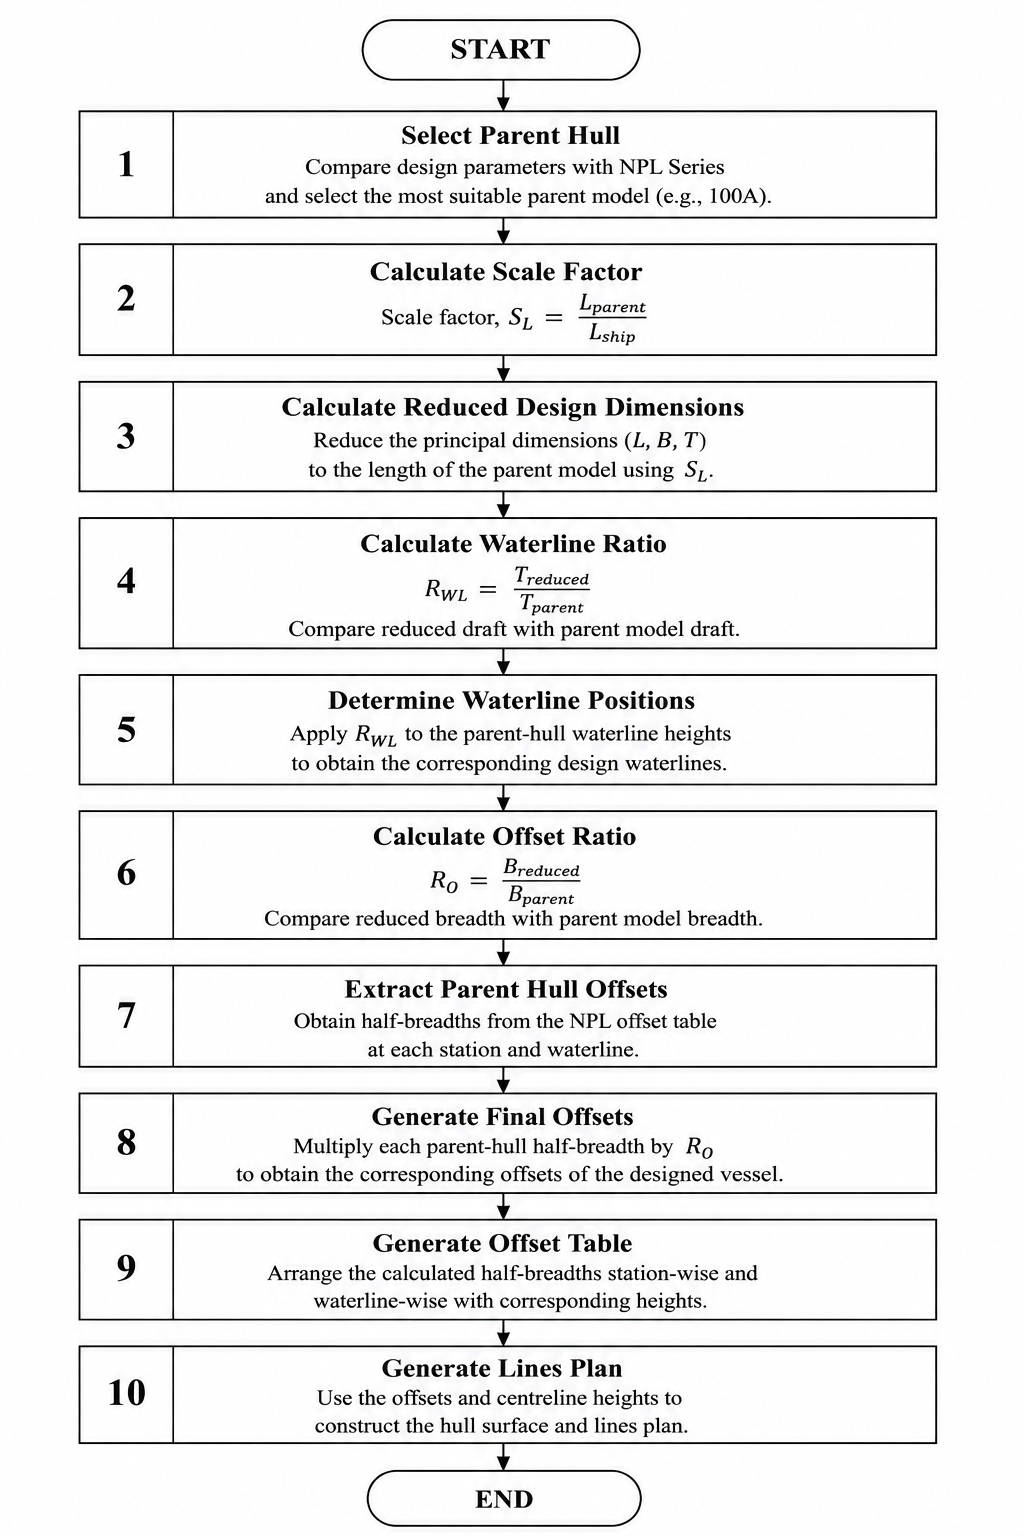
\includegraphics[width=0.87\linewidth]{CHAPTER 3/flowchart.png}
    \caption{Flowchart of Offset Generation}
    \label{fig:flowchart of offset generation}
\end{figure}


\begin{table}[H]
\centering
\caption{Generated Offset Table}
\label{tab:offset_table}
\vspace{2mm}

\resizebox{\textwidth}{!}{%
\begin{tabular}{c|ccccccccccc}
\toprule
\textbf{Station} &
\textbf{0} &
\textbf{0.5} &
\textbf{1} &
\textbf{1.5} &
\textbf{2} &
\textbf{3} &
\textbf{LWL} &
\textbf{4} &
\textbf{5} &
\textbf{6} &
\textbf{MDK} \\
\midrule

0    & 0 & 0 & 0 & 0 & 1.93 & 5.69 & 6.14 & 6.21 & 6.25 & 6.28 & 6.30 \\
0.5  & 0 & 0 & 0 & 0 & 2.28 & 5.82 & 6.24 & 6.37 & 6.42 & 6.45 & 6.47 \\
1    & 0 & 0 & 0 & 0 & 2.62 & 5.96 & 6.40 & 6.52 & 6.57 & 6.61 & 6.63 \\
1.5  & 0 & 0 & 0 & 0 & 2.95 & 6.11 & 6.53 & 6.65 & 6.71 & 6.75 & 6.78 \\
2    & 0 & 0 & 0 & 0 & 3.28 & 6.26 & 6.65 & 6.76 & 6.84 & 6.89 & 6.92 \\
3    & 0 & 0 & 0 & 0.64 & 3.97 & 6.45 & 6.85 & 6.99 & 7.11 & 7.17 & 7.22 \\
4    & 0 & 0 & 0 & 2.00 & 4.54 & 6.74 & 7.07 & 7.20 & 7.35 & 7.42 & 7.47 \\
5    & 0 & 0 & 0 & 2.79 & 4.95 & 6.94 & 7.23 & 7.36 & 7.53 & 7.62 & 7.68 \\
6    & 0 & 0 & 0 & 3.19 & 5.25 & 7.05 & 7.34 & 7.48 & 7.67 & 7.78 & 7.84 \\
7    & 0 & 0 & 0.74 & 3.65 & 5.49 & 7.13 & 7.44 & 7.57 & 7.77 & 7.89 & 7.96 \\
8    & 0 & 0 & 1.97 & 4.07 & 5.61 & 7.17 & 7.48 & 7.61 & 7.83 & 7.97 & 8.06 \\
9    & 0 & 0 & 2.49 & 4.24 & 5.57 & 7.04 & 7.40 & 7.58 & 7.85 & 8.02 & 8.14 \\
10   & 0 & 0 & 2.62 & 4.19 & 5.38 & 6.79 & 7.22 & 7.46 & 7.80 & 8.03 & 8.18 \\
11   & 0 & 0.61 & 2.61 & 3.98 & 5.06 & 6.47 & 6.94 & 7.22 & 7.66 & 7.97 & 8.17 \\
12   & 0 & 1.20 & 2.50 & 3.65 & 4.61 & 6.02 & 6.53 & 6.85 & 7.41 & 7.84 & 8.12 \\
13   & 0 & 1.27 & 2.26 & 3.21 & 4.05 & 5.41 & 5.97 & 6.33 & 7.04 & 7.65 & 8.05 \\
14   & 0.01 & 1.06 & 1.94 & 2.73 & 3.45 & 4.70 & 5.29 & 5.70 & 6.55 & 7.34 & 7.88 \\
15   & 0.18 & 0.88 & 1.59 & 2.24 & 2.85 & 3.97 & 4.55 & 4.98 & 5.92 & 6.85 & 7.54 \\
16   & 0 & 0.68 & 1.23 & 1.75 & 2.25 & 3.21 & 3.74 & 4.15 & 5.11 & 6.16 & 6.98 \\
17   & 0 & 0.43 & 0.88 & 1.25 & 1.63 & 2.41 & 2.85 & 3.21 & 4.12 & 5.25 & 6.17 \\
18   & 0 & 0.16 & 0.49 & 0.79 & 1.08 & 1.68 & 2.03 & 2.32 & 3.06 & 4.07 & 5.00 \\
18.5 & 0 & 0 & 0.26 & 0.55 & 0.79 & 1.24 & 1.51 & 1.76 & 2.47 & 3.40 & 4.28 \\
19   & 0 & 0 & 0 & 0.24 & 0.45 & 0.85 & 1.08 & 1.26 & 1.87 & 2.67 & 3.49 \\
19.5 & 0 & 0 & 0 & 0 & 0 & 0.38 & 0.61 & 0.78 & 1.26 & 1.93 & 2.67 \\
20   & 0 & 0 & 0 & 0 & 0 & 0 & 0 & 0.11 & 0.44 & 0.98 & 1.49 \\

\bottomrule
\end{tabular}%
}
\end{table}

\vspace{\baselineskip}\par\noindent After applying the calculated scale, waterline, and offset ratios to the NPL parent-hull data, the resulting half-breadths were arranged according to the corresponding stations and waterlines to form the generated offset table. The table represents the transverse dimensions of the hull at different longitudinal and vertical positions and therefore provides the basic geometric information required for constructing the hull surface.

\vspace{\baselineskip}\par\noindent The offsets at the intermediate stations describe the variation of the hull width along its length, while the waterline values define the change in the hull width with draft. The values near the forward and aft ends reduce progressively towards the ends of the vessel, ensuring a smooth transition of the hull form. The generated offsets were subsequently checked for continuity and consistency before being used for hull modeling.

\vspace{\baselineskip}\par\noindent In addition to the sectional half-breadths, keel and stern offsets are required to completely define the longitudinal profile of the hull. These offsets provide the corresponding vertical or longitudinal reference dimensions in the keel and stern regions and complement the sectional offset table. The calculated keel and stern offsets used to complete the hull geometry are presented in the following Table ~\ref{tab:keel_stem_offsets}
\begin{table}[H]
\centering
\caption{Keel and Stem Offsets}
\label{tab:keel_stem_offsets}

\begin{minipage}[t]{0.48\textwidth}
\centering
\textbf{Keel Offset}

\vspace{2mm}

\begin{tabular}{cc}
\toprule
\textbf{Station} & \textbf{Offset (m)} \\
\midrule
0    & 2.71 \\
0.5  & 2.61 \\
1    & 2.51 \\
1.5  & 2.42 \\
2    & 2.32 \\
3    & 2.13 \\
4    & 1.93 \\
5    & 1.73 \\
6    & 1.54 \\
7    & 1.35 \\
8    & 1.16 \\
9    & 0.96 \\
10   & 0.77 \\
11   & 0.58 \\
12   & 0.38 \\
13   & 0.17 \\
14   & 0 \\
15   & 0 \\
16   & 0 \\
17   & 0.19 \\
18   & 0.39 \\
18.5 & 0.78 \\
19   & 1.50 \\
19.5 & 3.06 \\
20   & 5.53 \\
\bottomrule
\end{tabular}

\end{minipage}
\hfill
\begin{minipage}[t]{0.48\textwidth}
\centering
\textbf{Sterm Offset}

\vspace{2mm}

\begin{tabular}{cc}
\toprule
\textbf{Waterline} & \textbf{Offset (m)} \\
\midrule
WL 4 & 0.39 \\
WL 5 & 1.46 \\
WL 6 & 2.38 \\
MDK  & 3.00 \\
\bottomrule
\end{tabular}


\end{minipage}

\end{table}
\section{Hull Model Development}
After generating the final offsets, a three-dimensional hull model was developed to verify the generated geometry and its hydrostatic characteristics. The modeling was carried out using Rhino, followed by hydrostatic verification in Maxsurf Modeler. Developing the hull model is an important step because the resulting geometry is used as the basis for several subsequent stages of ship design, including hydrostatics, stability analysis, resistance and propulsion estimation, weight and displacement verification, and further structural and performance studies.
\subsection{Lines Plan Development}
The hull line plan was prepared using **AutoCAD** based on the final offsets generated from the NPL Series. The calculated station- and waterline-wise offsets were plotted accurately in AutoCAD to develop the **body plan, profile plan, and half-breadth plan**. The offset coordinates were used to establish the corresponding stations, waterlines, and hull curves, which were then adjusted to obtain a smooth and continuous representation of the hull geometry. AutoCAD was used for accurate drafting, alignment, and final preparation of the line plan. \cite{autocad}

\subsection{Hull Modelling in Rhino}
The hull geometry generated from the final offsets was modeled in **Rhinoceros (Rhino)** to obtain a three-dimensional representation of the vessel hull. The station and waterline curves obtained from the offset data were imported and used to construct the hull surface, with the surface subsequently positioned to obtain a smooth and continuous hull form. The developed hull model was then transferred to **Maxsurf** for naval architectural analysis and verification of the principal hull characteristics. Maxsurf was used to evaluate the hull geometry and generate the required hydrostatic information, providing a check on the consistency of the developed hull form with the design parameters. \cite{rhino,maxsurf}


\begin{figure}[htbp]
    \centering

    \begin{minipage}{0.48\textwidth}
        \centering
        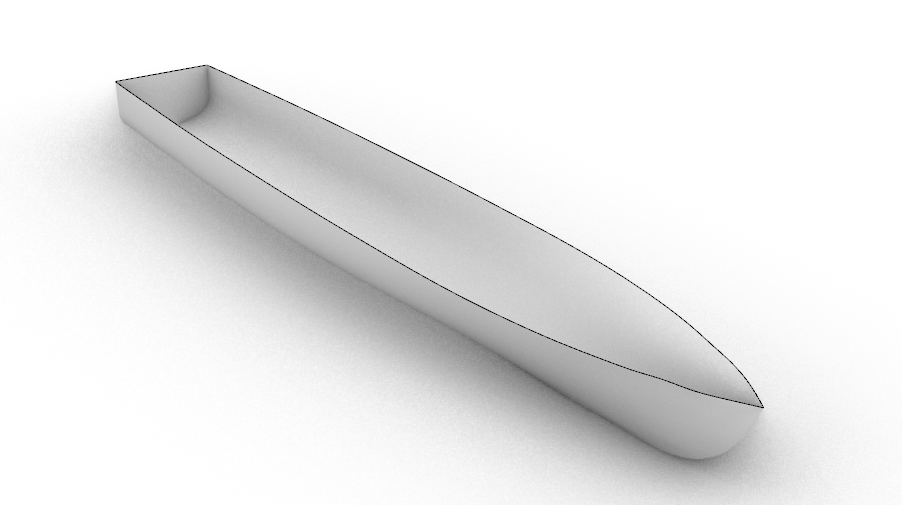
\includegraphics[width=\textwidth]{CHAPTER 3/RHINO MODEL.png}
        \caption{Model Generated in Rhino \cite{rhino}}
        \label{fig:rhino_model}
    \end{minipage}
    \hfill
    \begin{minipage}{0.48\textwidth}
        \centering
        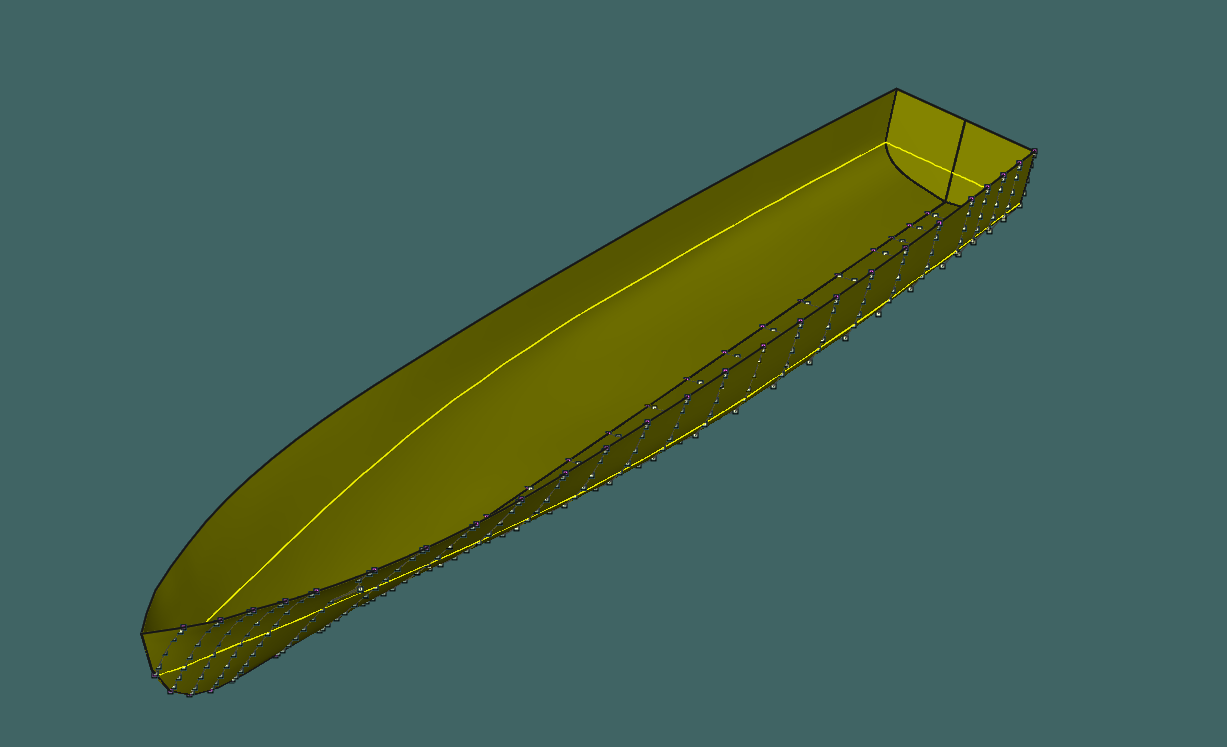
\includegraphics[width=\textwidth]{CHAPTER 3/MAXSURF MODEL.png}
        \caption{Model Generated in Maxsurf \cite{maxsurf}}
        \label{fig:maxsurf_model}
    \end{minipage}

\end{figure}



\vspace{\baselineskip}\par\noindent After importation, the hull was positioned with respect to the design waterline (LWL). The LWL was checked to ensure that it intersected the hull in the intended design draft and that the underwater portion of the model represented the required displacement condition. The imported surface was also inspected for gaps, discontinuities, or unwanted edges, since any surface defect can affect the accuracy of the hydrostatic calculations.
\subsection{Hydrostatic Verification}
Once the geometry was verified, Maxsurf was used to calculate the hydrostatic characteristics of the imported hull at the LWL. The displacement, volume, waterplane area, LCB, LCF, KB, and other hydrostatic parameters obtained from Maxsurf were compared with the corresponding values obtained from offset-based Excel calculations. This comparison provided an additional check on the accuracy of the hull geometry generated from the NPL offsets.

\vspace{\baselineskip}\par\noindent The hydrostatic results obtained from both methods showed close agreement for the major parameters, confirming the consistency of the independently calculated values with the Maxsurf results. The differences between the two sets of results were evaluated to quantify the deviation and identify any significant discrepancies. This verification process established confidence in the developed hull model and confirmed that the generated geometry was suitable for further hydrostatic and stability analysis.

\begin{figure}[htbp]
    \centering
    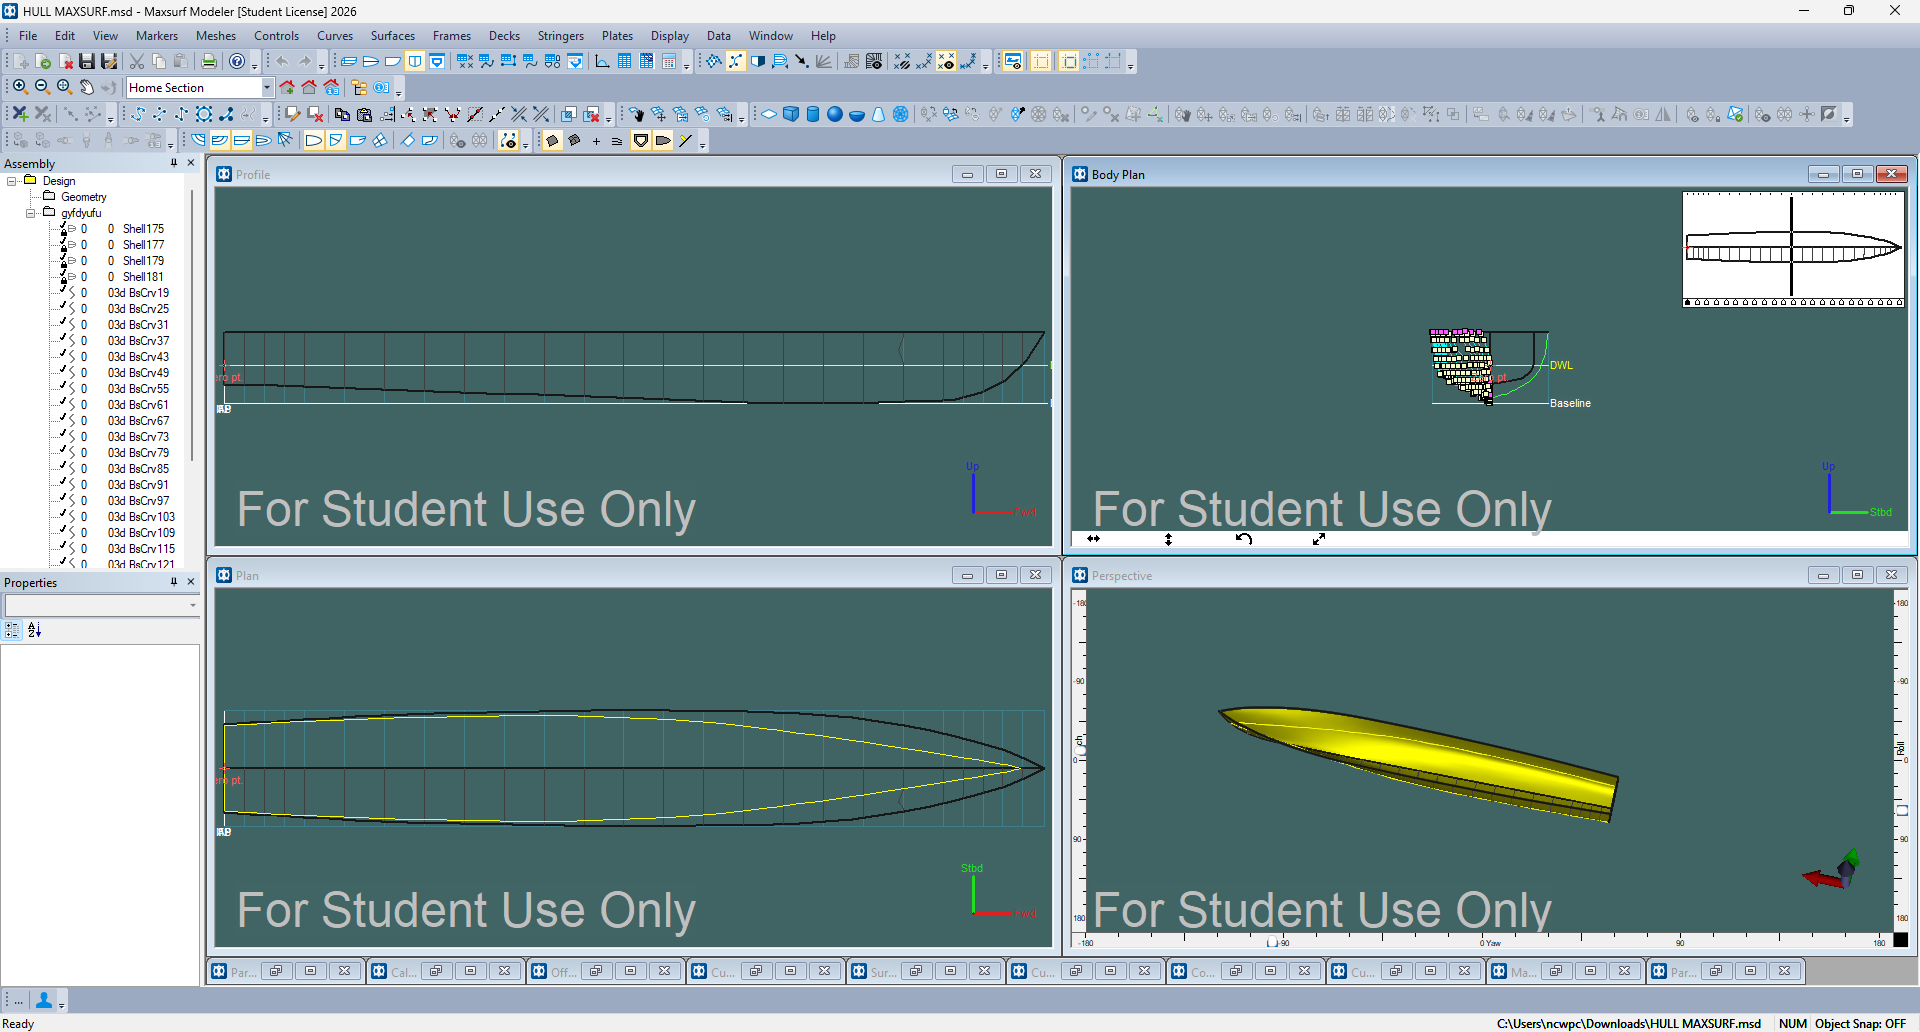
\includegraphics[width=1\linewidth]{CHAPTER 3/maxsurf interface.png}
    \caption{MAXSURF Interface Rhino \cite{rhino}}
    \label{fig:MAXSURF Interface}
\end{figure}


\begin{table}[H]
\centering
\caption{Hydrostatics obtained from MAXSURF}
\label{tab:hydrostatics_dwl}
\renewcommand{\arraystretch}{1.15}
\begin{tabular}{c l c c}
\hline
\textbf{No.} & \textbf{Measurement} & \textbf{Value} & \textbf{Unit} \\
\hline
1  & Displacement              & 3601       & t \\
2  & Volume (displaced)        & 3613.600   & m$^3$ \\
3  & WL Length                 & 112.675    & m \\
4  & Beam max extent           & 14.951     & m \\
5  & Waterpl. Area             & 1279.157   & m$^2$ \\
6  & Waterpl. Ixx (trans.)     & 18406.610  & m$^4$ \\
7  & Waterpl. Iyy (long.)      & 972862.25  & m$^4$ \\
8  & Prismatic coeff. ($C_P$)  & 0.684      & -- \\
9  & Block coeff. ($C_B$)      & 0.398      & -- \\
10 & Midship coeff. ($C_M$)    & 0.696      & -- \\
11 & Waterpl. area coeff.      & 0.759      & -- \\
12 & LCB length                & 49.378     & from AP \\
13 & LCF length                & 46.986     & from AP \\
14 & LCB \%                    & 43.824     & from AP \\
15 & LCF \%                    & 41.700     & from AP \\
16 & VCB                       & -1.625     & m \\
17 & VCF                       & 0.000      & m \\
18 & KB                        & 3.735      & m \\
19 & KG fluid                  & 5.350      & m \\
20 & BMT                       & 5.239      & m \\
21 & BML                       & 276.093    & m \\
22 & GMt corrected             & 3.613      & m \\
23 & GML                       & 276.267    & m \\
24 & KMt                       & 8.973      & m \\
25 & KML                       & 280.627    & m \\
26 & Immersion (TPC)           & 13.111     & tonnes/m \\
\hline
\end{tabular}
\end{table}


\vspace{\baselineskip}\par\noindent This verification also confirms that the design draft, waterline position, hull dimensions, and underwater volume have been correctly represented in the three-dimensional model. Any significant difference between the hydrostatics obtained from the offset calculations and those obtained from the Maxsurf model would indicate a possible error in the hull geometry or modeling process.
\vspace{\baselineskip}\par\noindent Therefore, hydrostatic verification acts as a validation step between hull-form generation and subsequent ship-design analysis. Once the model is verified, the same hull geometry can be confidently used for further calculations such as stability, resistance, propulsion, weight-displacement analysis, and other performance studies.

\subsection{Aim of Model generation}
The purpose of generating a model in Rhino is to create an accurate 3D 
geometric representation of the hull of the ship that can be imported into Maxsurf for detailed 
hydrostatic and stability analysis. By developing a precise surface model in Rhino, 
essential parameters such as volume, center of buoyancy, and waterplane area can be 
accurately computed in Maxsurf. These calculated hydrostatic properties and stability 
values are then used to validate the manual calculations to ensure accuracy in the ship design process and to confirm the reliability of both the numerical model and hand
derived results. Furthermore, a model is essential to perform CFD calculations.  
\vspace{\baselineskip}\par\noindent For the project, the verification of the area up to the main deck was validated 
with the area obtained from the rhino by making a planar surface in the rhino, and the hydrostatics 
were validated with the hydrostatic values obtained from Maxsurf.

\section{Lines Plan}
Lines plan is a set of technical drawings used to represent the three-dimensional geometry of a ship's hull in two-dimensional views. It is prepared from the generated hull offsets and provides a clear representation of the hull shape at different stations, waterlines, and longitudinal sections. The line plan is an important reference for hull construction, hull fairness check, and hull geometry communication developed. 
\vspace{\baselineskip}\par\noindent A conventional lines plan consists of three principal drawings:
\subsection{Body Plan}
The body plan shows the transverse sections of the hull at different stations when viewed from the forward and aft ends. It represents the variation of the hull's breadth and shape along its length. The body plan is particularly useful for checking the fairness and continuity of the individual hull sections.

\vspace{\baselineskip}\par\noindent The body plan is an important component of the line plan as it provides a transverse view of the hull of the ship at different stations along its length. It clearly represents the shape and variation of the hull sections from the keel to the deck and from the centreline to the sides. The body plan is useful for determining the sectional geometry, checking the fairness and continuity of hull curves, and obtaining important hydrostatic properties such as sectional areas, displacement, center of buoyancy, and moments. It also helps to accurately construct and develop the structural structure of the hull.

\begin{figure}[htbp]
    \centering
    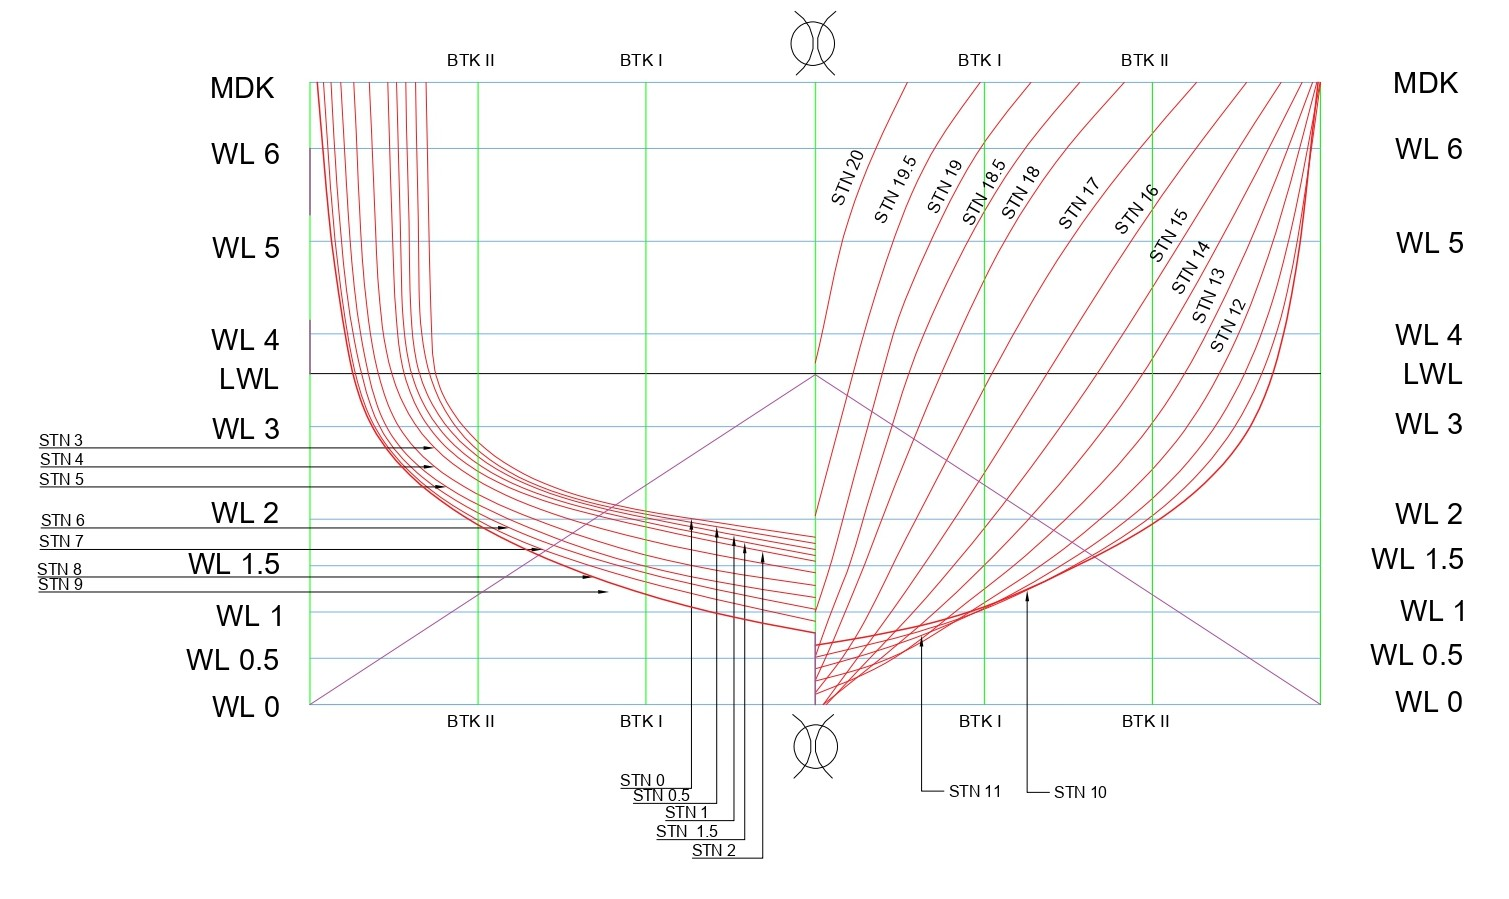
\includegraphics[width=1\linewidth]{CHAPTER 3/BODYPLAN_page-0001.jpg}
    \caption{Body Plan \cite{autocad}}
    \label{fig:body plan}
\end{figure}

\subsection{Half-Breadth Plan}
The half-breadth plan is a view of the hull from above and shows the positions of the waterlines along the length of the vessel. Since the hull is generally symmetrical about the centreline, only one half of the hull is normally represented. It illustrates how the breadth of the hull varies at different longitudinal positions and waterlines.
\begin{figure}[htbp]
    \centering
    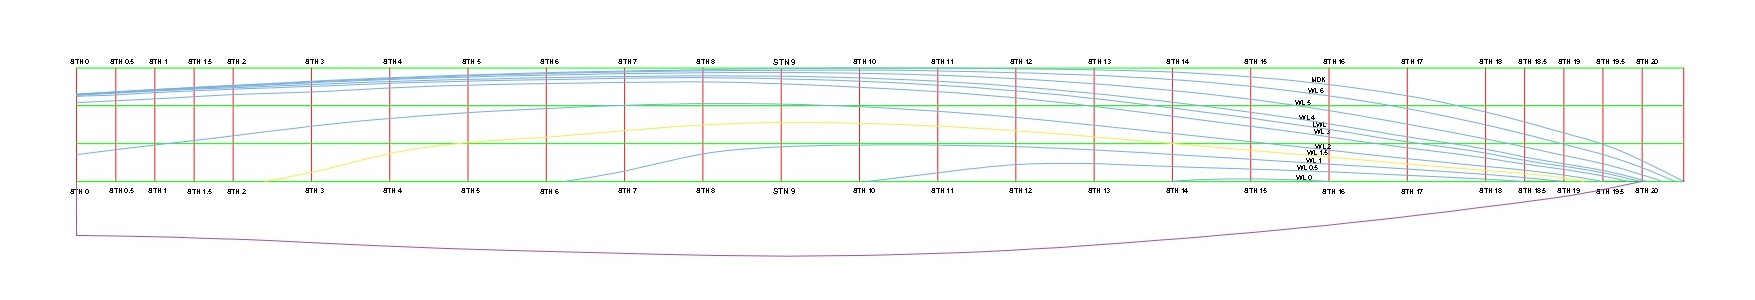
\includegraphics[width=1\linewidth]{CHAPTER 3/HALF BREADTH PLAN_page-0001.jpg}
    \caption{Half Breadth Plan \cite{autocad}}
    \label{fig:half breadth plan}
\end{figure}
\subsection{Sheer Plan}
The sheer plan, also called the profile plan, shows the hull from the side. It represents the longitudinal profile of the vessel, including the keel line, stem, stern, deck, or sheer line, and waterlines. Provides the longitudinal reference required to define the overall form and vertical dimensions of the hull.
\begin{figure}[htbp]
    \centering
    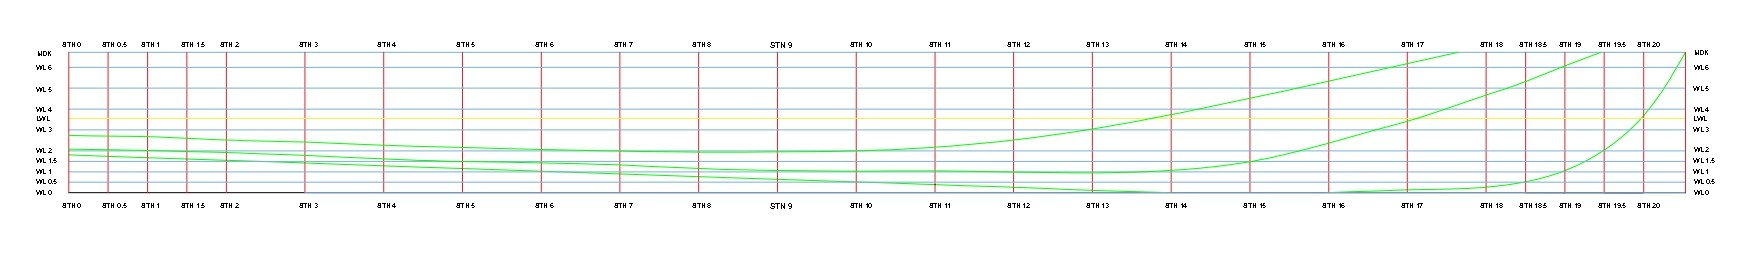
\includegraphics[width=1\linewidth]{CHAPTER 3/SHEER PLAN_page-0001.jpg}
    \caption{Sheer Plan \cite{autocad}}
    \label{fig:sheer plan}
\end{figure}
\vspace{\baselineskip}\par\noindent Together, these three views provide a complete representation of the hull geometry. The body plan describes the transverse shape, the half-breadth plan describes the plan-view shape, and the sheer plan describes the longitudinal profile. The three drawings are mutually related and are used together to verify that the hull geometry generated from the NPL offsets is consistent and fair.


\section{Bonjean Curves}
Bonjean curves are a set of curves that are used to represent the submerged sectional area of a ship at different drafts along its length. For each station of the vessel, a curve is plotted showing how the underwater sectional area changes as the draft increases. Thus, the Bonjean diagram provides a convenient way of representing the longitudinal and vertical distribution of the underwater volume of the hull.
\vspace{\baselineskip}\par\noindent The sectional areas required for the construction of the Bonjean curves are obtained from the hull geometry at different stations and waterlines. The curves therefore provide a direct relationship between draft, sectional area, and longitudinal position, allowing the underwater geometry of the vessel to be evaluated for different loading conditions.
\subsection{Applications of Bonjean Curves}
Bonjean curves are used mainly for the following:
\begin{enumerate}[\alph*)]
    \item \textbf{Displacement Calculation : }Bonjean curves provide the sectional areas at different drafts and stations. These sectional areas can be integrated along the length of the vessel to determine the underwater volume and displacement.
    \item \textbf{Determination of LCB : }The sectional areas obtained from the Bonjean curves are used to determine the longitudinal distribution of buoyancy. From this distribution, the Longitudinal Centre of Buoyancy (LCB) can be calculated.
    \item \textbf{Buoyancy Distribution : }Bonjean curves show how the underwater sectional area varies along the length of the ship for a particular draft. This helps in determining the distribution of buoyancy along the vessel.
    \item \textbf{Longitudinal Strength Analysis : }The buoyancy distribution obtained from Bonjean curves can be compared with the weight distribution to determine the net load distribution along the ship. This is useful for calculating longitudinal shear forces and bending moments.
    \item \textbf{Damage Stability Analysis : }Bonjean curves provide sectional information about the underwater portion of the hull. This information can be used when analysing changes in buoyancy and displacement after flooding of different compartments.
    \item \textbf{Trim and Loading Analysis : }Since the curves provide sectional areas at different drafts, they can be used to evaluate changes in displacement and buoyancy distribution when the vessel operates at different drafts or trim conditions.
\end{enumerate}

\section{Bonjean Calculations}
The Bonjean areas have been calculated using the methods mentioned below.    
\subsection{Area using Simpson's rules}
The area up to WL 0.5 for each station was calculated using the
trapezoidal rule.

\begin{equation}
\mathrm{AREA}_{0.5}
=
2 \times 0.5 \times h \times (y_0+y_{0.5})
\end{equation}

\vspace{\baselineskip}\par\noindent where

\begin{align*}
h &= 0.5 \\
y_0 &= \text{half ordinate at WL 0 for a station} \\
y_{0.5} &= \text{half ordinate at WL 0.5 for a station}
\end{align*}

\vspace{\baselineskip}\par\noindent The area up to WL 6 was calculated using Simpson's rule.
Simpson's rules $1,3,3,1$ and $1,4,1$ were used to calculate the area
of the water line up to waterline 6.

\vspace{\baselineskip}\par\noindent For Simpson's $1,3,3,1$ rule:

\begin{equation}
A =
3 \times \frac{h \times \sum f(x)}{8}
\end{equation}

\vspace{\baselineskip}\par\noindent For Simpson's $1,4,1$ rule:

\begin{equation}
A =
\frac{h \times \sum f(x)}{3}
\end{equation}

\vspace{\baselineskip}\par\noindent It was also found that using Simpson's $1,3,3,1$ and $1,4,1$ rules,
the obtained area was more accurate compared to the $5,8,-1$ rule.

\vspace{\baselineskip}\par\noindent The areas obtained from Simpson's rules were also compared with the
areas obtained by plotting a planar surface between the stations and
the centreline at various stations, and the area up to the main deck
was compared.
\begin{table}[H]
\centering
\caption{Bonjean Areas}
\vspace{2mm}
\label{tab:sectional_areas}

\resizebox{\textwidth}{!}{%
\begin{tabular}{c|ccccccccccc}
\toprule
\textbf{STN/WL} &
\textbf{0} &
\textbf{0.5} &
\textbf{1} &
\textbf{1.5} &
\textbf{2} &
\textbf{3} &
\textbf{LWL} &
\textbf{4} &
\textbf{5} &
\textbf{6} &
\textbf{MDK} \\
\midrule

0    & 0 & 0 & 0 & 0.24125 & 0.965 & 13.0275 & 23.0865 & 33.23 & 50.3689 & 68.65876 & 82.11935 \\
0.5  & 0 & 0 & 0 & 0.285 & 1.14 & 14.2875 & 24.4837 & 34.37 & 52.74 & 71.3025 & 85.1269 \\
1    & 0 & 0 & 0 & 0.3275 & 1.31 & 15.5475 & 25.9719 & 35.6 & 55.05 & 73.8675 & 88.03608 \\
1.5  & 0 & 0 & 0 & 0.36875 & 1.475 & 16.83 & 27.4868 & 36.99 & 57.33 & 76.3875 & 90.8646 \\
2    & 0 & 0 & 0 & 0.41 & 1.64 & 18.1125 & 28.9933 & 38.36 & 59.52 & 78.80625 & 93.58473 \\
3    & 0 & 0 & 0.08 & 0.06375 & 3.265 & 20.655 & 31.8592 & 40.73 & 63.77 & 83.565 & 98.96052 \\
4    & 0 & 0 & 0.25 & 1.1825 & 6.27 & 22.905 & 34.5292 & 43.24 & 67.54 & 87.94125 & 103.8736 \\
5    & 0 & 0 & 0.39875 & 2.135 & 9.005 & 25.65 & 37.753 & 46.18 & 72.29125 & 93.465 & 110.1802 \\
6    & 0 & 0 & 0.39875 & 2.135 & 9.005 & 25.65 & 37.753 & 46.18 & 72.29125 & 93.465 & 110.1802 \\
7    & 0 & 0.08 & 0.19125 & 3.6175 & 10.785 & 29.07 & 41.3424 & 50.11 & 75.24125 & 97.7625 & 114.7238 \\
8    & 0 & 0.25 & 1.215 & 5.815 & 12.915 & 33.64875 & 45.97435 & 55.39 & 78.235 & 102.7913 & 119.9434 \\
9    & 0 & 0.39875 & 1.64875 & 6.74875 & 13.755 & 35.1225 & 47.2703 & 56.84 & 78.66875 & 104.1413 & 121.4325 \\
10   & 0 & 0.39875 & 1.76875 & 6.92375 & 13.69 & 34.63875 & 46.42355 & 55.86 & 77.12875 & 102.8138 & 120.1602 \\
11   & 0 & 0.28375 & 2.7775 & 7.75625 & 14.32 & 33.165 & 44.4448 & 53.66 & 75.1075 & 99.63 & 116.9016 \\
12   & 0 & 0.8875 & 3.68125 & 8.3175 & 14.505 & 30.76875 & 41.32475 & 50.15 & 71.47125 & 94.48875 & 111.5695 \\
13   & 0 & 0.9875 & 3.64 & 7.75625 & 13.245 & 27.3825 & 36.9543 & 45.11 & 65.28 & 87.19875 & 104.0031 \\
14   & 0 & 0.82375 & 3.085 & 6.59625 & 11.25 & 23.49 & 31.8886 & 39.17 & 57.575 & 78.37875 & 94.66772 \\
15   & 0 & 0.79375 & 2.65375 & 5.53125 & 9.345 & 19.65375 & 26.81195 & 33.1 & 49.42375 & 68.61375 & 84.00748 \\
16   & 0 & 0.52625 & 1.9625 & 4.2 & 7.215 & 15.35625 & 21.19145 & 26.41 & 40.3225 & 57.15 & 71.1991 \\
17   & 0 & 0.32 & 1.3125 & 2.90875 & 5.055 & 11.1825 & 15.5953 & 19.63 & 30.4925 & 44.53875 & 56.7421 \\
18   & 0 & 0.20375 & 0.80375 & 1.79375 & 3.175 & 7.155 & 10.1566 & 12.93 & 20.73375 & 31.3425 & 41.0153 \\
18.5 & 0 & 0.03 & 0.14125 & 0.74625 & 1.72 & 4.77 & 7.1024 & 9.18 & 15.33125 & 24.1875 & 32.35695 \\
19   & 0 & 0 & 0.04125 & 0.2275 & 0.905 & 2.61 & 4.227 & 5.62 & 10.44875 & 17.06625 & 23.61822 \\
19.5 & 0 & 0 & 0 & 0 & 0 & 0.48375 & 1.29295 & 2.46 & 5.08 & 9.88875 & 14.76973 \\
20   & 0 & 0 & 0 & 0 & 0 & 0 & 0.0252 & 0.13 & 1 & 3.16125 & 5.946817 \\
\bottomrule
\end{tabular}%
}
\end{table}



\subsection{Area obtained from RHINO}
The Bonjean areas of the vessel were calculated independently using an Excel-based approach. The sectional areas at different stations and waterline levels were determined from the corresponding hull dimensions and sectional geometry. These calculations were carried out systematically for all the stations to obtain the sectional area distribution required for the preparation of the Bonjean curves and for subsequent hydrostatic calculations.

\vspace{\baselineskip}\par\noindent To validate Excel-based calculations, the sectional areas of the hull were also obtained from the three-dimensional hull model developed in Rhino. The area up to the main deck was determined for each station using the sectioning and area-measurement functions available in Rhino. The values obtained from Rhino were then tabulated along with the corresponding values calculated using Excel.

\vspace{\baselineskip}\par\noindent Subsequently, a station-wise comparison was performed between the Rhino and Excel results. The difference between the two values was calculated for each station, followed by the corresponding percentage difference. This comparison provides a direct measure of the agreement between the geometrically obtained sectional areas from Rhino and the independently calculated values from Excel. The results show close agreement at most of the stations, with the percentage differences generally remaining within a small range.

\vspace{\baselineskip}\par\noindent The comparison serves as a validation of Excel-based Bonjean area calculations and helps identify any discrepancies arising from geometric interpretation, numerical approximation, or measurement of sectional areas. The close correspondence between the two methods indicates that the Excel procedure can satisfactorily reproduce the sectional area distribution obtained from the Rhino hull model. These validated Bonjean areas can subsequently be used for further hydrostatic calculations and analysis of the vessel's hull form.

\begin{table}[H]
\centering
\caption{Comparison of Bonjean Areas Obtained from Rhino and Excel}
\vspace{2mm}
\label{tab:rhino_excel_bonjean}

\small
\setlength{\tabcolsep}{4pt}

\begin{tabular}{c c c c}
\hline

\textbf{RHINO} &
\textbf{EXCEL} &
\textbf{DIFFERENCE} &
\textbf{PERCENTAGE} \\

\hline

83.6454061  & 82.11935   & 1.5260561  & 1.858339234 \\
85.944850  & 85.126900   & 0.8175845  & 0.960402518 \\
88.3086881  & 88.0360833  & 0.2726048  & 0.309651175 \\
90.9034518  & 90.8646000  & 0.0388518  & 0.042759057 \\
93.4916162  & 93.5847333  & -0.0931171 & -0.09950346 \\
98.0685243  & 98.9605167  & -0.8931171 & -0.904090234 \\
104.495040  & 103.8375500  & 0.6205490  & 0.597779996 \\
109.079794  & 110.1801833  & -1.1003893 & -0.978718009 \\
112.467250  & 110.1801833  & 2.285217  & 2.071626310 \\
115.6431830 & 114.7247833  & 0.9183997  & 0.801402848 \\
118.6753540 & 119.9433500  & -1.2679960 & -1.057162402 \\
119.6451650 & 121.4324500  & -1.7872850 & -1.471834753 \\
118.5143100 & 120.1602333  & -1.6188023 & -1.347203054 \\
115.6994190 & 116.9015833  & -1.2021643 & -1.028355903 \\
111.0938730 & 111.5695167  & -0.4756437 & -0.426320451 \\
103.9877350 & 104.0031000  & -0.0153650 & -0.014773598 \\
92.1707576  & 94.6677167   & -2.4969591 & -2.637603562 \\
83.9649890  & 84.0074833   & -0.0424943 & -0.050589866 \\
71.3297323  & 71.1991000   & 0.1306323  & 0.183474651 \\
56.6341820  & 56.7421000   & -0.1079180 & -0.19042611 \\
40.9735133  & 41.0153000   & -0.0417867 & -0.101880762 \\
32.3527945  & 32.3569500   & -0.0041555 & -0.012842681 \\
23.9193660  & 23.6182167   & 0.2957433  & 1.252208571 \\
14.9372268  & 14.7697333   & 0.1674935  & 1.134031759 \\
5.8722996   & 5.9468167    & -0.0745171 & -1.253505583 \\

\hline
\end{tabular}

\end{table}



\subsection{Moment calculations using Simpson's rules}
The moment of area, or the first moment of area, was also calculated
using Simpson's rule. The moment up to waterline three for each station
was calculated using Simpson's $3,10,-1$ rule, and beyond waterline three
was calculated using Simpson's rule.

\vspace{\baselineskip}\par\noindent Simpson's $3,10,-1$ rule provides the moment between the first two
ordinates when three equally spaced ordinates are available.

\begin{equation}
\text{Simpson's }3,10,-1\text{ rule:}
\qquad
M = \frac{h^2}{24}\times\sum f(x)
\end{equation}

\vspace{\baselineskip}\par\noindent In Bonjean analysis, moment of area converts sectional area data into
hydrostatic levels and stiffness measures needed to locate the center
of buoyancy, compute transverse metacentric radius, and build righting
capability across drafts, trims, and heel angles. By taking first and
second moments of the waterplane and immersed-sectional areas about
reference axes, Bonjean tables become directly usable for displacement,
LCB/LCF, KM, and stability curve construction, linking geometry to
equilibrium and strength checks in design and loading.
\begin{table}[H]
\centering
\caption{Bonjean Momnets}
\vspace{2mm}
\label{tab:first_moments}

\resizebox{\textwidth}{!}{%
\begin{tabular}{c|ccccccccccc}
\toprule
\textbf{STN/WL} &
\textbf{0} &
\textbf{0.5} &
\textbf{1} &
\textbf{1.5} &
\textbf{2} &
\textbf{3} &
\textbf{LWL} &
\textbf{4} &
\textbf{5} &
\textbf{6} &
\textbf{MDK} \\
\midrule

0    & 0 & 0 & 0 & 0.361875 & 7.599375 & 67.76438 & 96.58432 & 197.5568 & 328.5593 & 478.8218 & 566.9693 \\
0.5  & 0 & 0 & 0 & 0.4275   & 10.08    & 71.7518  & 100.81303 & 204.1003 & 338.6278 & 492.9853 & 583.5162 \\
1    & 0 & 0 & 0 & 0.49125  & 12.45375 & 75.61875 & 105.5521 & 211.1483 & 348.8033 & 506.8283 & 599.6151 \\
1.5  & 0 & 0 & 0 & 0.553125 & 14.69813 & 80.09813 & 110.6715 & 218.4615 & 359.0115 & 520.4115 & 615.1995 \\
2    & 0 & 0 & 0 & 0.615    & 16.9425  & 84.6075  & 115.7887 & 225.4912 & 368.6587 & 533.2762 & 630.0398 \\
3    & 0 & 0 & 0.09 & 0.065625 & 22.58438 & 93.59438 & 125.6977 & 238.9852 & 387.6202 & 588.8542 & 659.6112 \\
4    & 0 & 0 & 0.28125 & 1.68 & 28.1475 & 103.3875 & 136.6171 & 253.5833 & 407.1008 & 584.1983 & 688.482 \\
5    & 0 & 0 & 0.392344 & 2.602969 & 31.92047 & 110.093 & 144.1265 & 263.8303 & 420.9928 & 602.5753 & 709.7141 \\
6    & 0 & 0 & 0.448594 & 3.052969 & 34.49672 & 114.4017 & 148.9493 & 270.5618 & 430.5293 & 615.6368 & 725.0315 \\
7    & 0 & 0.069375 & 0.111094 & 4.422656 & 38.38641 & 119.8214 & 154.8498 & 277.9623 & 439.9623 & 627.5523 & 738.5404 \\
8    & 0 & 0.184688 & 1.089844 & 6.315469 & 42.54047 & 124.4105 & 159.6081 & 283.2756 & 446.4006 & 635.5956 & 747.7949 \\
9    & 0 & 0.233438 & 1.504688 & 7.123125 & 43.77938 & 124.1419 & 158.8767 & 281.618 & 444.8705 & 634.823 & 747.8767 \\
10   & 0 & 0.245625 & 1.621406 & 7.241719 & 42.90047 & 120.203 & 153.9729 & 274.1642 & 435.9167 & 625.1792 & 738.5393 \\
11   & 0 & 0.04125 & 2.014219 & 7.396406 & 41.00391 & 114.3464 & 146.712 & 262.4858 & 420.6683 & 607.2608 & 720.0354 \\
12   & 0 & 0.328125 & 2.327344 & 7.298906 & 37.91391 & 105.7364 & 136.0837 & 245.2574 & 397.3799 & 578.9624 & 690.3364 \\
13   & 0 & 0.383438 & 2.229375 & 6.619688 & 33.45094 & 93.93094 & 121.5304 & 221.5391 & 364.8116 & 538.9541 & 648.2909 \\
14   & 0 & 0.315 & 1.898906 & 5.636719 & 28.40672 & 80.49422 & 104.7909 & 193.8721 & 325.8196 & 489.6271 & 595.3211 \\
15   & 0 & 0.263438 & 1.562813 & 4.625625 & 23.32313 & 66.92813 & 87.69812 & 164.6969 & 282.6944 & 432.4619 & 532.0025 \\
16   & 0 & 0.203438 & 1.206094 & 3.591094 & 18.23859 & 53.18859 & 70.16524 & 133.6677 & 234.2952 & 365.4627 & 455.9436 \\
17   & 0 & 0.119063 & 0.82875 & 2.528438 & 13.03219 & 38.99719 & 51.8662 & 100.425 & 180.3075 & 288.18 & 366.3761 \\
18   & 0 & 0.076875 & 0.500625 & 1.56375 & 8.2125 & 25.445 & 34.24461 & 67.46211 & 125.3396 & 206.4671 & 268.0564 \\
18.5 & 0 & 0.0225 & 0.125156 & 0.823594 & 5.398594 & 14.48859 & 25.30712 & 50.96087 & 97.47587 & 164.0609 & 215.8738 \\
19   & 0 & 0 & 0.046406 & 0.325781 & 3.044531 & 11.84953 & 16.62141 & 34.58391 & 69.21891 & 120.4439 & 161.7917 \\
19.5 & 0 & 0 & 0 & 0 & 0.48375 & 3.24375 & 5.6315 & 15.82025 & 38.43275 & 73.97525 & 104.5264 \\
20   & 0 & 0 & 0 & 0 & 0 & 0.195 & 0.282212 & 0.777478 & 8.157478 & 23.57748 & 40.49028 \\

\bottomrule
\end{tabular}%
}
\end{table}

\begin{figure}[htbp]
    \centering
    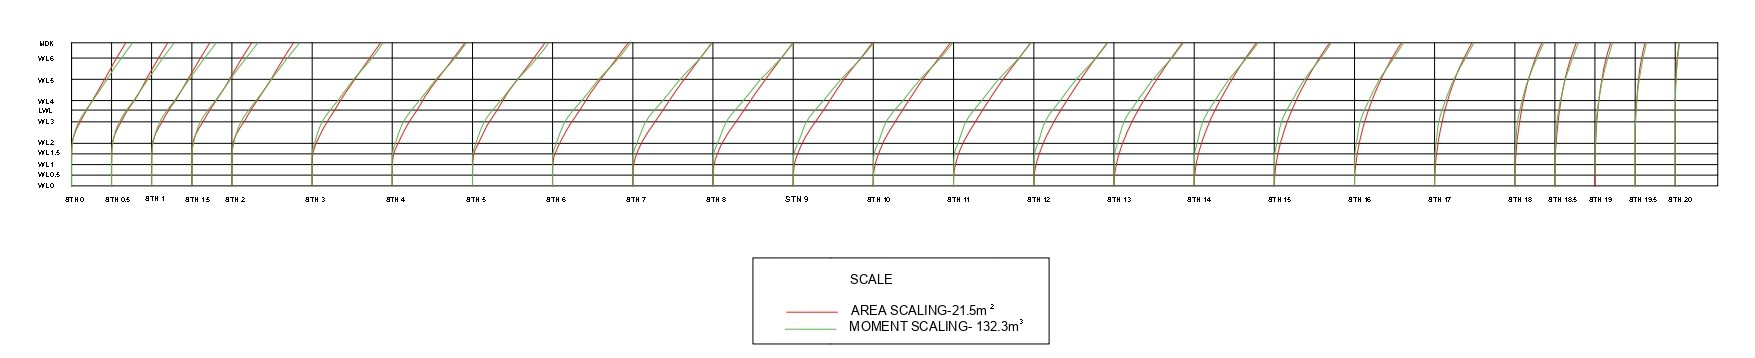
\includegraphics[width=1\linewidth]{CHAPTER 3/BONJEANS_page-0001.jpg}
    \caption{Bonjean Curves \cite{autocad}}
    \label{fig:placeholder}
\end{figure}

\subsection{Bonjeans obtained from MASSPROP}

% -----------------------------------------------------------
% SECTIONAL AREA AND MOMENT COMPARISON
% -----------------------------------------------------------

The sectional properties of the hull at different stations were determined
using the \texttt{MASSPROP} command in AutoCAD and compared with the
values obtained by numerical calculations in Excel. For each station,
the hull section was represented as a closed region before applying the
\texttt{MASSPROP} command. The command provides the sectional area,
centroidal location, moments of inertia, and other geometric properties of
the selected section. The sectional area represents the underwater
cross-sectional area of the hull at the respective station, while the
moment provides a measure of the distribution of this area about the
reference axis.

\vspace{\baselineskip}\par\noindent The values obtained from AutoCAD were compared with the corresponding
values calculated in Excel using sectional offsets and numerical
integration procedures. This comparison provides an independent check of
the accuracy of the hull geometry and the numerical calculations. Small
differences between the two methods can occur due to differences in the
geometric representation of the curves, the interpolation of offsets, and
numerical integration. However, the overall agreement between the two sets
of values confirms that the geometry of the developed station and the calculated
sectional properties are consistent.

\vspace{\baselineskip}\par\noindent The comparison of sectional area and moment values at the different
stations is presented in Table~\ref{tab:massprop_excel}. Subsequently, these values are used in the hydrostatic analysis of the vessel, particularly
 to determine the distributions of sectional areas and to verify the
hydrostatic characteristics of the hull. The use of \texttt{MASSPROP}
therefore provides a reliable CAD-based verification of the manually
calculated sectional properties and helps to ensure the accuracy of the hull
model used in the present design study.

\begin{table}[H]
\centering
\caption{Comparison of Sectional Area and Moment Obtained from MASSPROP and Excel}
\vspace{2mm}
\label{tab:massprop_excel}

\small
\setlength{\tabcolsep}{4pt}

\begin{tabular}{c c c c c}
\hline
\textbf{STN} &
\multicolumn{2}{c}{\textbf{MASSPROP}} &
\multicolumn{2}{c}{\textbf{EXCEL}} \\

\cline{2-5}

& \textbf{Area} & \textbf{Moment}
& \textbf{Area} & \textbf{Moment} \\

\hline

0    & 83.0644  & 558.2924 & 82.11935 & 566.9693 \\
0.5  & 85.7268  & 574.4039 & 85.1269  & 583.5162 \\
1    & 88.3109  & 589.7579 & 88.03608 & 599.6151 \\
1.5  & 90.8929  & 604.4105 & 90.8646  & 615.1995 \\
2    & 93.4945  & 618.6999 & 93.58473 & 630.0398 \\
3    & 98.6829  & 645.8697 & 98.96052 & 659.6112 \\
4    & 104.2922 & 674.9270 & 103.8736  & 688.4820 \\
5    & 109.0883 & 697.3906 & 110.1802  & 709.7141 \\
6    & 112.8115 & 714.2886 & 110.1802  & 725.0315 \\
7    & 116.1719 & 727.6311 & 114.7238  & 738.5404 \\
8    & 118.6667 & 736.4099 & 119.9434  & 747.87949 \\
9    & 119.6457 & 738.0465 & 121.4325  & 747.8767 \\
10   & 118.5372 & 731.0189 & 120.1602  & 738.5393 \\
11   & 115.6933 & 714.9615 & 116.9016  & 720.0354 \\
12   & 111.0954 & 688.7804 & 111.5695  & 690.3364 \\
13   & 103.7889 & 651.5348 & 104.0031  & 648.2909 \\
14   & 94.7186  & 694.7704 & 94.66772  & 595.3211 \\
15   & 83.9648  & 728.3527 & 84.00748  & 532.0025 \\
16   & 71.3282  & 605.1841 & 71.1991   & 455.9436 \\
17   & 56.6325  & 384.4497 & 56.7421   & 366.3761 \\
18   & 41.3486  & 288.4065 & 41.0153   & 268.0564 \\
18.5 & 32.5266  & 232.6888 & 32.35695  & 215.8738 \\
19   & 23.5827  & 175.6345 & 23.61822  & 161.7917 \\
19.5 & 14.9101  & 117.9359 & 14.76973  & 104.5264 \\
20   & 5.5580   & 48.32014 & 5.946817  & 40.49028 \\

\hline
\end{tabular}

\end{table}

\subsection{Features of Bonjean Curves}
The curves are plotted on the sheer plan of the ship with the draft on the vertical axis 
and the area (or the moment of the area) on the horizontal, one set per station arrayed along 
the length; differing horizontal and vertical scales are commonly used to keep the 
drawing compact and readable. 
\vspace{\baselineskip}\par\noindent Smooth, fuller curves near midship indicate higher area growth with draft 
and thus stronger buoyancy contribution, whereas finer bow/stern curves show slower 
growth, shaping the longitudinal buoyancy lever and affecting trim. 
\vspace{\baselineskip}\par\noindent Inclusion of vertical moments with the area curves accelerates computation 
of hydrostatic levers needed for KM/GM and righting moment development across 
drafts and trims in early design stages.

\section{Hydrostatics}
Hydrostatics deals with the behavior of a vessel when it is at rest in water and describes the relationship between the hull geometry and its buoyancy characteristics. Hydrostatic curves are graphical representations of important hydrostatic parameters plotted against the draft of the vessel. They provide a convenient way to understand how the underwater characteristics of the hull change as the vessel's draft varies.
\vspace{\baselineskip}\par\noindent The commonly plotted hydrostatic parameters include displacement, volume of displacement, waterplane area, LCB, LCF, KB, BM, KM, and TPC. These curves are generated from the geometry of the hull and provide the necessary information to evaluate the vessel under different loading conditions.
\subsection{Uses of Hydrostatic Curves}
Hydrostatic curves are used to determine the displacement and buoyancy characteristics of the vessel at different drafts. They help in checking whether the hull can provide the required buoyancy for the intended loading condition.

\vspace{\baselineskip}\par\noindent They are also used in stability calculations, particularly for obtaining parameters such as \(KB\), \(BM\), \(KM\), and metacentric height. These values are required to assess the initial stability of the vessel at different drafts.

\vspace{\baselineskip}\par\noindent The curves provide LCB and LCF information, which is useful to analyze the longitudinal position of buoyancy and flotation. This is important when studying the trim and loading conditions of the vessel.

\vspace{\baselineskip}\par\noindent Hydrostatic curves are also used during weight and displacement verification, as well as in subsequent stability and loading calculations. Thus, they provide the basic hydrostatic data required for several later stages of the ship design process.\cite{roh2018shipstability}

\begin{enumerate}[\alph*)]

\item \textbf{Volume of displacement} $(\nabla)$
\begin{equation}
\nabla =
\left(\frac{1}{3}\right)
(\text{station spacing})
\sum f(V)
\end{equation}

\item \textbf{Mass displacement} $(\Delta)$
\begin{equation}
\Delta = \nabla \times (1.006) \times (1.025)
\end{equation}

\item \textbf{Transverse moment of inertia} $(I_T)$
\begin{equation}
I_T =
\left(\frac{2}{9}\right)
(\text{station spacing})
\sum f(I_T)
\end{equation}

\item \textbf{Longitudinal moment of inertia} $(I_L)$
\begin{equation}
I_L =
\left[
\left(\frac{2}{3}\right)
(\text{station spacing})
\sum f(I_L)
\right]
-
\left[AWP \times (LCF)^2\right]
\end{equation}

\item \textbf{Tons per cm immersion} $(TPC)$
\begin{equation}
TPC =
\frac{AWP \times 1.025}{100}
\end{equation}

\item \textbf{Moment causing a trimming of 1 cm} $(MCT)$
\begin{equation}
MCT =
\frac{\Delta \times {GM_L}}{LBP \times 100}
\end{equation}

\item \textbf{Longitudinal metacentric radius} $(BM_L)$
\begin{equation}
BM_L = \frac{I_L}{\nabla}
\end{equation}

\item \textbf{Transverse metacentric radius} $(BM_T)$
\begin{equation}
BM_T = \frac{I_T}{\nabla}
\end{equation}

\item \textbf{Longitudinal Center of Buoyancy} $(LCB)$
\begin{equation}
LCB = \frac{\sum f(M)}{\sum f(V)}
\end{equation}

\item \textbf{Longitudinal Center of Flotation} $(LCF)$
\begin{equation}
LCF =
h \times
\frac{\sum f(M)}{\sum f(A)}
\end{equation}

\item \textbf{Vertical Center of Buoyancy} $(VCB)$
\begin{equation}
VCB =
h \times
\frac{\sum f(M)}{\sum f(V)}
\end{equation}

\item \textbf{Block coefficient} $(C_B)$
\begin{equation}
C_B =
\frac{\nabla}{L \times B \times T}
\end{equation}

\item \textbf{Prismatic coefficient} $(C_P)$
\begin{equation}
C_P =
\frac{\nabla}{A_{\text{midships}} \times L}
\end{equation}

\item \textbf{Midship coefficient} $(C_M)$
\begin{equation}
C_M =
\frac{A_{\text{midships}}}{B \times T}
\end{equation}

\item \textbf{Waterplane area coefficient} $(C_W)$
\begin{equation}
C_W =
\frac{AWP}{L \times B}
\end{equation}

\end{enumerate}

\begin{table}[H]
\centering
\caption{Hydrostatics}
\vspace{2mm}
\label{tab:hydrostatic_particulars}

\resizebox{\textwidth}{!}{%
\begin{tabular}{lrrrrrrrrrrr}
\toprule
\textbf{Parameter} &
\textbf{WL 0} &
\textbf{WL 0.5} &
\textbf{WL 1} &
\textbf{WL 1.5} &
\textbf{WL 2} &
\textbf{WL 3} &
\textbf{LWL} &
\textbf{WL 4} &
\textbf{WL 5} &
\textbf{WL 6} &
\textbf{MDK} \\
\midrule

MOMENT &
0 & 2450.903 & 10266.38 & 26943.71 & 52855.57 &
126225.4 & 174578.9 & 214192.7 & 316317.7 & 429235.2 & 517408.9 \\

VOLUME &
0 & 33.21258 & 145.5911 & 420.5083 & 912.0136 &
2479.658 & 3519.019 & 4360.03 & 6486.426 & 8673.824 & 10348.68 \\

MASS &
0 & 34.0429 & 149.2309 & 431.021 & 934.8139 &
2541.649 & 3606.994 & 4469.03 & 6648.587 & 8890.669 & 10607.4 \\

$I_T$ &
0.029292 & 23.37902 & 377.3441 & 1930.003 & 5746.626 &
15316.66 & 18404.11 & 20132.69 & 23366.47 & 26681.42 & 29612.49 \\

AREA &
2.787333 & 71.416 & 240.238 & 503.6033 & 826.369 &
1188.195 & 1279.461 & 1331.366 & 1430.166 & 1525.726 & 1600.419 \\

LCF &
84.5973 & 77.75306 & 66.7228 & 57.03584 & 48.63651 &
46.19513 & 46.98442 & 47.78763 & 49.79274 & 51.87801 & 53.46576 \\

VCB &
0.003784 & 0.073333 & 0.118658 & 0.013038 & 0.31396 &
0.59158 & 0.58823 & 0.56043 & 0.46346 & 0.34071 & -0.23462 \\

$I_L$ &
2.339833 & 7830.415 & 60144.95 & 222706 & 533078 &
874560.8 & 973830.2 & 1036714 & 1172478 & 1317525 & 1433521 \\

TPC &
0.02857 & 0.732014 & 2.46244 & 5.161934 & 8.470282 &
12.1719 & 13.11448 & 13.6465 & 14.6592 & 15.63869 & 16.40429 \\

$BM_L$ &
0 & 235.7665 & 413.1088 & 529.6115 & 584.5066 &
352.6941 & 276.7335 & 237.7769 & 180.7587 & 151.8967 & 138.522 \\

$BM_T$ &
0 & 0.703921 & 2.591808 & 4.589691 & 6.301031 &
6.176923 & 5.229897 & 4.617558 & 3.602364 & 3.076086 & 2.861475 \\

MCT &
0 & 0.002124 & 0.034289 & 0.175377 & 0.522189 &
1.391806 & 1.672359 & 1.829433 & 2.132283 & 2.424509 & 2.690852 \\

LCB &
0 & 73.79441 & 70.51519 & 64.07414 & 57.95481 &
50.90436 & 49.4101 & 49.12644 & 48.7661 & 49.4862 & 49.99756 \\

$C_B$ &
0 & 0.390672 & 0.321638 & 0.231504 & 0.246138 &
0.343124 & 0.389879 & 0.421065 & 0.481272 & 0.517326 & 0.54152 \\

$C_P$ &
0 & 0.542 & 0.562 & 0.637964 & 0.605187 &
0.63922 & 0.671898 & 0.688357 & 0.734743 & 0.72728 & 0.742448 \\

$C_M$ &
0 & 0.221528 & 0.280754 & 0.36288 & 0.406714 &
0.536785 & 0.580266 & 0.611695 & 0.655021 & 0.711317 & 0.72937 \\

$C_W$ &
0.685185 & 0.630037 & 0.796096 & 0.623815 & 0.669072 &
0.739877 & 0.758668 & 0.77145 & 0.795853 & 0.818979 & 0.84332 \\

KB &
0 & 0.3975 & 0.795 & 1.1925 & 1.59 &
2.385 & 2.83656 & 3.18 & 3.975 & 4.77 & 5.3371 \\

KMT &
0 & 1.101421 & 3.386808 & 5.782191 & 7.891031 &
8.561923 & 8.066457 & 7.797558 & 7.577364 & 7.846086 & 8.198575 \\

KML &
0 & 236.164 & 413.9038 & 530.804 & 586.0966 &
355.0791 & 279.57 & 240.9569 & 184.7337 & 156.6667 & 143.8591 \\

\bottomrule
\end{tabular}%
}
\end{table}
\begin{figure}[htbp]
    \centering
    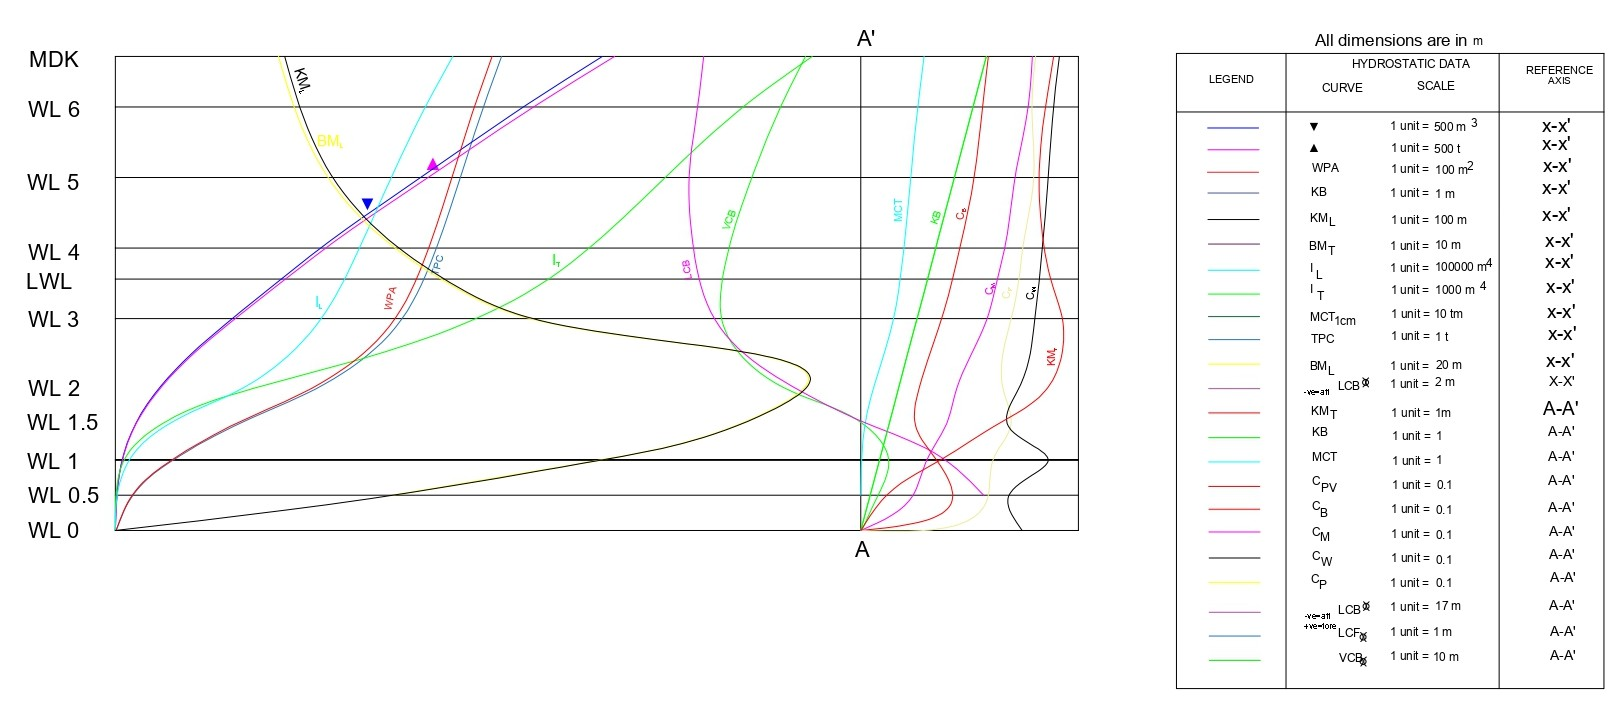
\includegraphics[width=1\linewidth]{CHAPTER 3/HYDROSTATICS_page-0001.jpg}
    \caption{Hydrostatics \cite{autocad}}
    \label{fig:hydrostatics}
\end{figure}




\subsection{Hydrostatics from Maxsurf Stability}
The hydrostatic details of the designed vessel were first calculated independently using an Excel-based approach. The required hydrostatic parameters were obtained by applying the relevant naval architecture formulae to the principal dimensions, displacement, waterplane properties, and sectional characteristics of the vessel. The calculations were systematically organized in Excel to determine parameters such as displacement, volume of displacement, waterplane area, coefficients, centers of buoyancy and flotation, metacentric heights and other relevant hydrostatic properties.

\vspace{\baselineskip}\par\noindent To Validate Excel-based calculations, the same vessel model and the corresponding hydrostatic condition were analyzed using Maxsurf Stability. The hydrostatic parameters obtained from both methods were then compared on a parameter-by-parameter basis. The percentage error between the Excel results and the Maxsurf results was calculated to assess the level of agreement between the two approaches. This comparison serves to verify the accuracy of the independently developed Excel calculations and to determine how closely the calculated hydrostatic particulars reproduce the results obtained from the established Maxsurf analysis.

\begin{figure}[htbp]
    \centering
    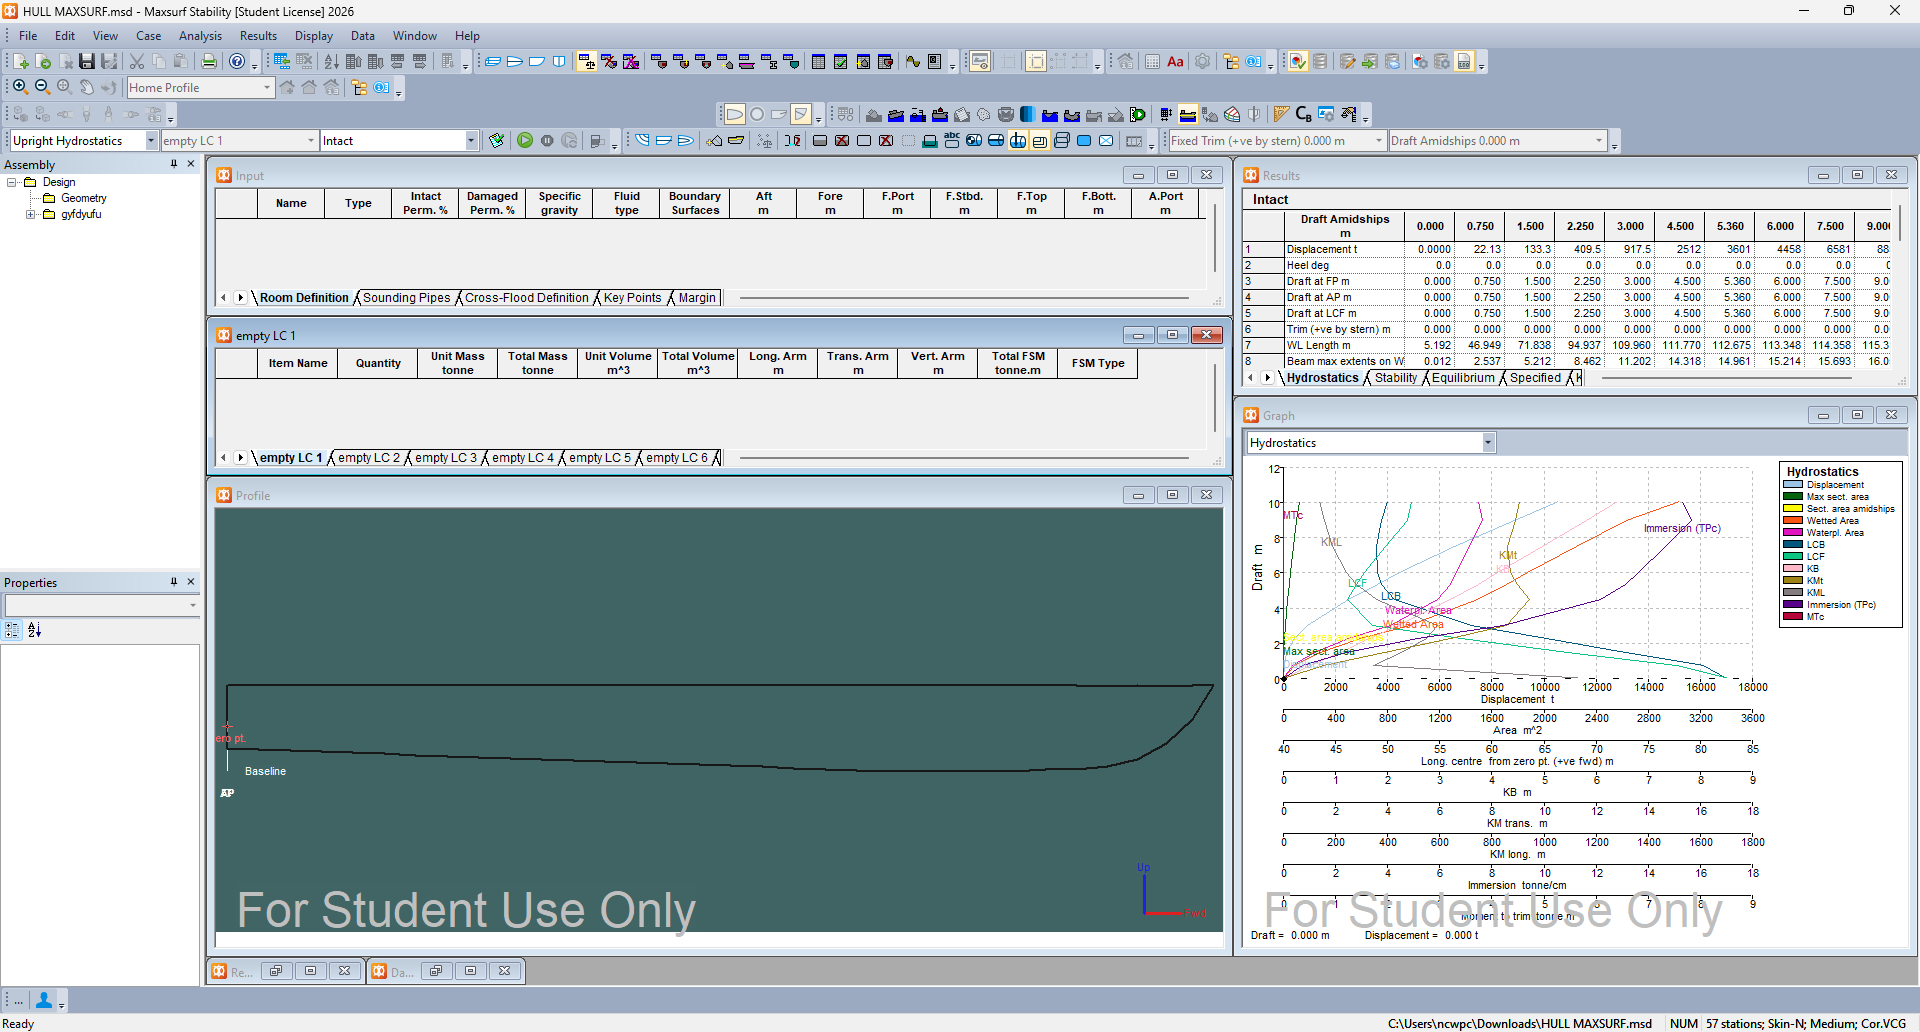
\includegraphics[width=1\linewidth]{CHAPTER 3/maxsurf stability interface.png}
    \caption{Interface of Maxsurf Stability \cite{maxsurf}}
    \label{fig : Interface of Maxsurf Stability}
\end{figure}

\begin{table}[H]
\centering
\caption{Hydrostatic values obtained from MAXSURF Stability}
\vspace{2mm}
\label{tab:excel_hydrostatics}
\resizebox{\textwidth}{!}{%
\begin{tabular}{lrrrrrrrrrrr}
\toprule
\textbf{Parameter} &
\textbf{WL 0} &
\textbf{WL 0.5} &
\textbf{WL 1} &
\textbf{WL 1.5} &
\textbf{WL 2} &
\textbf{WL 3} &
\textbf{LWL} &
\textbf{WL 4} &
\textbf{WL 5} &
\textbf{WL 6} &
\textbf{MDK} \\
\midrule
Displacement (t)
& 0 & 22.13 & 133.3 & 409.5 & 917.5 & 2512 & 3601 & 4458 & 6581 & 8852 & 10567 \\

WL Length (m)
& 5.192 & 46.949 & 71.838 & 94.937 & 109.96 & 111.77 & 112.675 & 113.348 & 114.358 & 115.315 & 115.998 \\

Beam max extent (m)
& 0.012 & 2.537 & 5.212 & 8.462 & 11.202 & 14.318 & 14.961 & 15.214 & 15.693 & 16.057 & 16.356 \\

Wetted Area (m$^2$)
& 0.029 & 86.789 & 284.425 & 591.246 & 966.066 & 1489.434 & 1714.362 & 1875.759 & 2251.22 & 2630.117 & 3040.266 \\

Waterpl. Area (m$^2$)
& 0.026 & 69.377 & 235.523 & 500.374 & 822.676 & 1185.106 & 1279.157 & 1330.154 & 1429.4 & 1526.188 & 1494.131 \\

Prismatic coeff. ($C_P$)
& 0.381 & 0.529 & 0.525 & 0.534 & 0.564 & 0.660 & 0.684 & 0.696 & 0.717 & 0.734 & 0.744 \\

Block coeff. ($C_B$)
& 0.191 & 0.241 & 0.231 & 0.221 & 0.242 & 0.340 & 0.389 & 0.420 & 0.477 & 0.518 & 0.539 \\

Max. sect. area coeff. ($C_M$)
& 0.500 & 0.557 & 0.588 & 0.580 & 0.605 & 0.664 & 0.696 & 0.717 & 0.757 & 0.786 & 0.799 \\

Waterpl. area coeff. ($C_{WP}$)
& 0.435 & 0.583 & 0.629 & 0.623 & 0.668 & 0.741 & 0.759 & 0.771 & 0.796 & 0.824 & 0.788 \\

LCB from zero point (m)
& 82.468 & 80.264 & 72.828 & 65.199 & 57.998 & 50.612 & 49.378 & 48.994 & 48.930 & 49.426 & 49.969 \\

LCF from zero point (m)
& 82.707 & 77.735 & 67.240 & 57.058 & 48.556 & 46.133 & 46.986 & 47.783 & 49.797 & 51.934 & 52.283 \\

KB (m)
& -0.001 & 0.524 & 1.087 & 1.650 & 2.207 & 3.214 & 3.735 & 4.109 & 4.964 & 5.809 & 6.415 \\

KG (m)
& 5.360 & 5.360 & 5.360 & 5.360 & 5.360 & 5.360 & 5.360 & 5.360 & 5.360 & 5.360 & 5.360 \\

BM$_T$ (m)
& 0.009 & 1.028 & 2.773 & 4.778 & 6.370 & 6.221 & 5.239 & 4.619 & 3.633 & 3.084 & 2.655 \\

BM$_L$ (m)
& 1161.935 & 345.345 & 452.240 & 548.485 & 588.583 & 354.595 & 276.093 & 238.227 & 182.735 & 153.207 & 133.144 \\

GM$_T$ (m)
& -5.352 & -3.808 & -1.500 & 1.068 & 3.217 & 4.074 & 3.613 & 3.368 & 3.237 & 3.533 & 3.710 \\

GM$_L$ (m)
& 1156.575 & 340.509 & 447.966 & 544.776 & 583.453 & 352.449 & 275.267 & 236.976 & 182.339 & 153.656 & 134.199 \\

KM$_T$ (m)
& 0.008 & 1.552 & 3.860 & 6.428 & 8.577 & 9.434 & 8.973 & 8.728 & 8.597 & 8.893 & 9.070 \\

KM$_L$ (m)
& 1161.935 & 345.869 & 453.326 & 550.136 & 590.790 & 357.809 & 280.627 & 242.336 & 187.699 & 159.016 & 139.559 \\

Immersion (TPC)
& 0 & 0.711 & 2.414 & 5.129 & 8.432 & 12.147 & 13.111 & 13.634 & 14.651 & 15.643 & 15.315 \\

RM at 1 deg (t-m)
& 0 & -1.471 & -3.490 & 7.635 & 51.515 & 178.620 & 227.105 & 262.023 & 371.823 & 545.859 & 684.150 \\

\hline
\end{tabular}%
}
\end{table}

\vspace{\baselineskip}\par\noindent Maxsurf Stability provides a dedicated hydrostatics plotting function that automatically generates hydrostatic curves from the hydrostatic values calculated by the software. These curves graphically represent the variation of important parameters with respect to displacement or draft, such as displacement, waterplane area, KB, BM, KM, GM, and other hydrostatic particulars. Automatically generated graphs provide a convenient visual representation of the hydrostatic characteristics of the vessel and can also be used alongside independently calculated Excel results for comparison and validation.

\begin{figure}
    \centering
    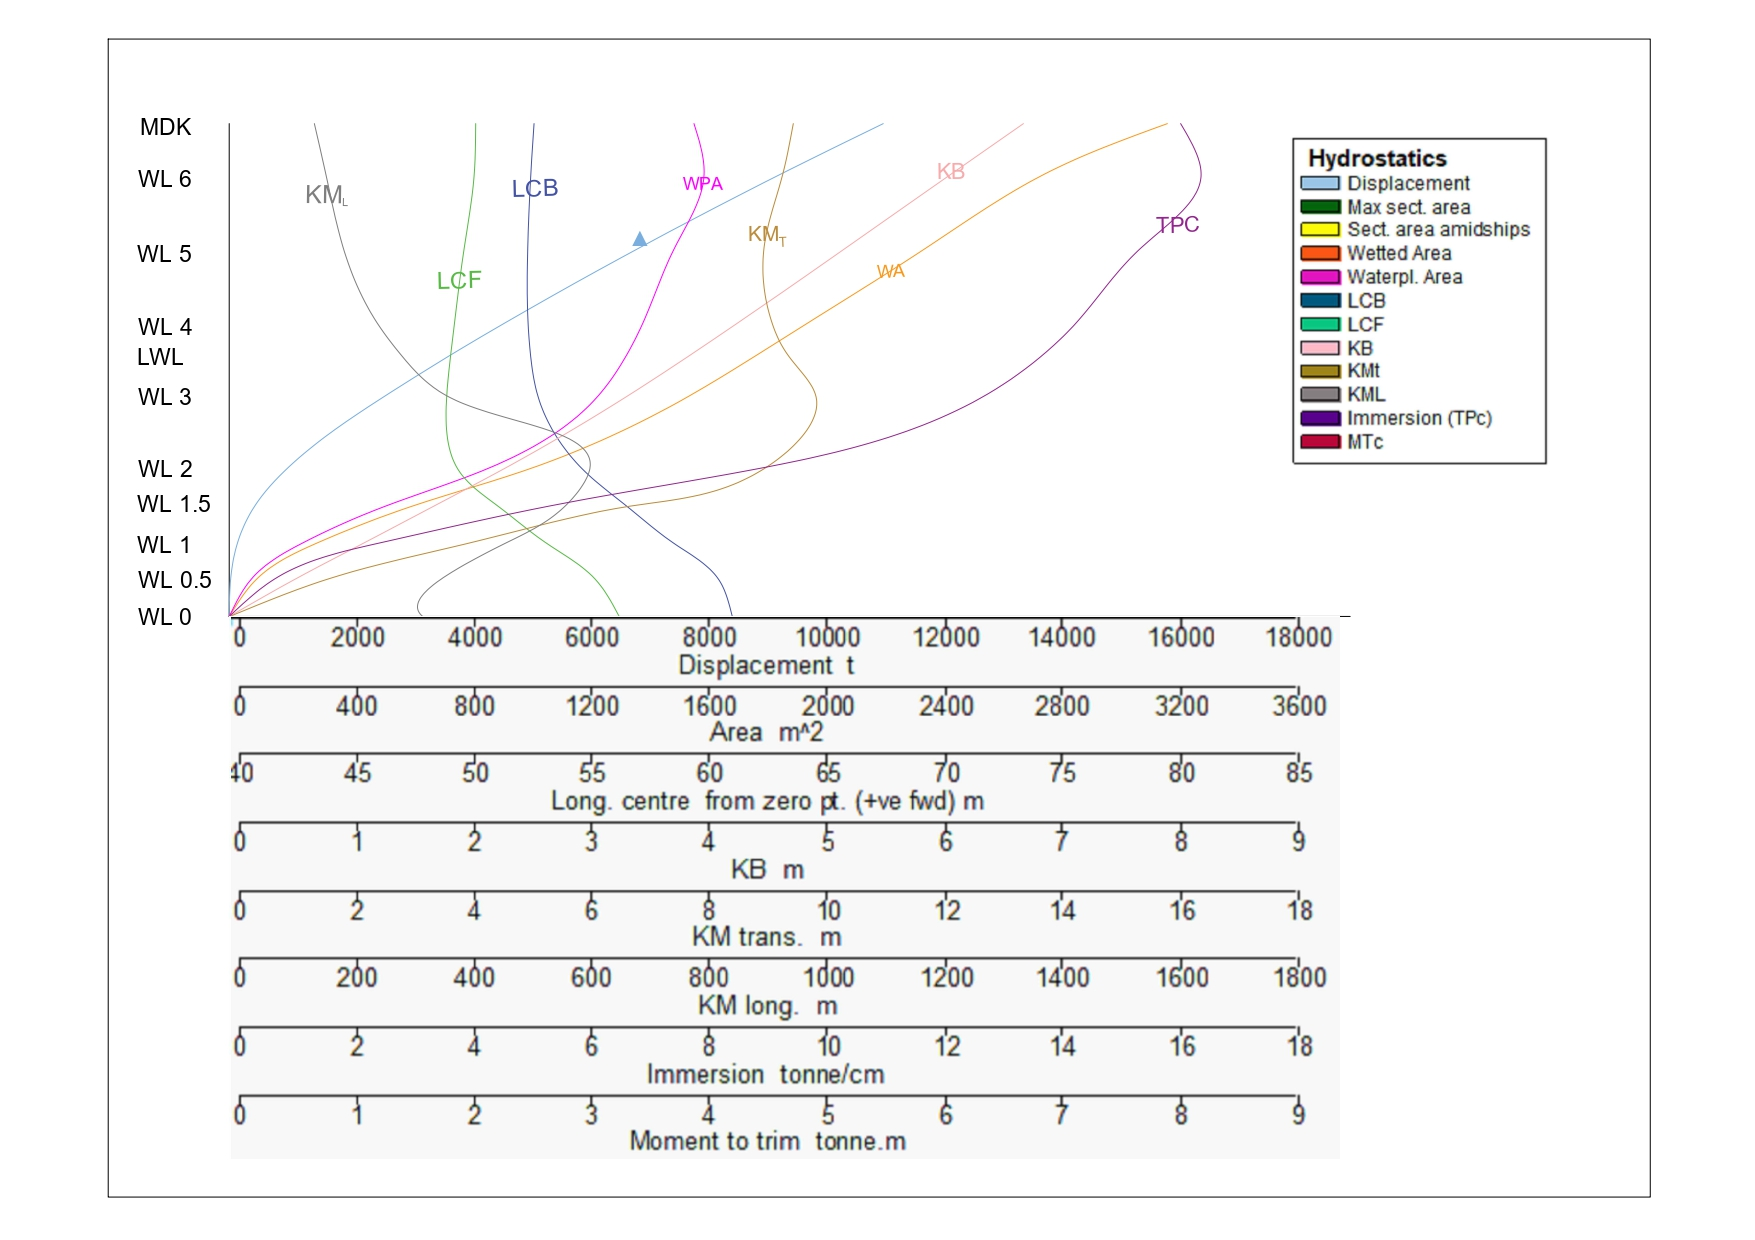
\includegraphics[width=1\linewidth]{CHAPTER 3/HYDROSTATICS FROM MAXSURF (1).jpg}
   \caption{Hydrostatic curves obtained from MAXSURF Stability \cite{maxsurf}\cite{autocad}}
    \label{fig:Hydrostatic curves obtained from MAXSURF Stability }
\end{figure}

\section{Conclusion}

This chapter presented the development and analysis of the hull geometry of the proposed vessel, beginning with the selection of a suitable hull form and progressing through the generation of offsets, lines plan, sectional properties, Bonjean data and hydrostatic characteristics. The hull form was developed with consideration of the main dimensions and the design requirements of the vessel. The NPL series was selected as the basis for the hull-form development because of its suitable geometric characteristics and its applicability to a high-speed naval vessel. The selected parent form was subsequently modified to obtain the required principal dimensions and displacement while maintaining a practical and hydrodynamically suitable hull geometry.

\vspace{\baselineskip}\par\noindent The hull geometry was developed using a combination of computational and CAD-based techniques. The offsets obtained from the hull-form generation procedure were used to construct the body plan, the half-width plan, and the sheer plan, thereby forming the complete lines plan of the vessel. The line plan provides an essential representation of the three-dimensional hull geometry and ensures that the transitions between stations, waterlines, and buttock lines are smooth and continuous. Particular attention was paid to the fairness of the hull surface because abrupt discontinuities or changes in curvature can adversely affect the resistance and flow characteristics of the vessel. The developed lines plan therefore serves as the fundamental geometric reference for the subsequent hydrostatic and hydrodynamic analysis.

\vspace{\baselineskip}\par\noindent The sectional characteristics of the hull were determined at the selected stations using the generated offsets. Sectional areas were evaluated using numerical integration techniques in Excel, while the corresponding geometric properties were also obtained directly from the CAD model. The use of AutoCAD's \texttt{MASSPROP} command provided an independent method for determining the area, centroidal location, and moments of the individual station sections. This approach was particularly useful for verifying the numerical calculations performed from the offset data. The comparison between the values obtained from \texttt{MASSPROP} and Excel showed reasonable agreement, confirming that the station geometry represented in the CAD model was consistent with the offset data used in the analytical calculations.

\vspace{\baselineskip}\par\noindent The Bonjean sectional areas were also generated for the hull at different stations and waterline levels. Bonjean data provide a convenient means of representing the variation of the draft-immersed sectional area and are particularly useful for determining the displacement and longitudinal distribution of the buoyancy under different loading conditions. The Bonjean areas obtained from the Rhino model were compared with the corresponding values calculated in Excel. The differences observed between the two methods were generally small and primarily attributed to differences in curve representation, interpolation, and numerical integration. The comparison therefore provided an additional validation of the developed hull geometry and the calculated sectional properties.

\vspace{\baselineskip}\par\noindent The hydrostatic analysis carried out using the sectional data is an important part of the overall design process. The calculated sectional areas were integrated along the length of the vessel to obtain the underwater volume and displacement characteristics. From hydrostatic calculations, important parameters can be determined, such as the longitudinal distribution of the buoyancy, the center of the buoyancy, the characteristics of the waterplane, and other principal hydrostatic coefficients. These parameters are essential to evaluate the suitability of the hull form in the selected design condition and provide the necessary foundation for subsequent stability, resistance, propulsion, and structural calculations.

\vspace{\baselineskip}\par\noindent An important outcome of this chapter is the establishment of a consistent computational workflow between the hull-form generation software, the CAD modeling environment, and the calculations based on spreadsheets. Rhino and AutoCAD were used for the geometric development and verification of the hull, while Excel was used for numerical calculations and systematic processing of the sectional data. The use of multiple methods for evaluating the same geometric quantities reduces the possibility of errors and provides greater confidence in the final results. The comparison of sectional areas and moments demonstrates that the developed hull model can be reliably used for further analysis and design calculations.

\vspace{\baselineskip}\par\noindent In general, the work presented in this chapter establishes the geometric and hydrostatic foundation of the proposed vessel. The final form of the hull satisfies the principal design requirements while maintaining a continuous and fair geometry suitable for further naval architectural analysis. The generated lines plan, offset table, sectional properties, Bonjean data, and hydrostatic calculations together provide a complete representation of the underwater hull geometry. The verification carried out using independent CAD and numerical methods further improves the reliability of the results. Consequently, the form of the hull developed in this chapter provides a suitable basis for subsequent stages of the design of the vessel, including resistance estimation, propulsion selection, stability assessment, structural design, and evaluation of the overall performance of the proposed vessel.
\section{Scope for Next Chapter}
With the hull geometry and hydrostatic characteristics established, the next chapter focuses on the resistance of the vessel. The developed hull form will be analyzed to determine its resistance characteristics at the required operating speeds.
\vspace{\baselineskip}\par\noindent The resistance analysis will include the selection of an appropriate resistance prediction method, the calculation of the major resistance components, and the estimation of the total resistance and the effective power required for the vessel. The results will subsequently provide the basis for the calculations of the propulsion system and the power requirement.

\begin{figure}[htbp]
    \centering

    \begin{minipage}{0.2\textwidth}
        \centering
        
\includegraphics[width=\linewidth]{CHAPTER 3/QR CODE.png}
    \end{minipage}
    \hfill
    \begin{minipage}{0.68\textwidth}
        \raggedright
        \textit{Scan the QR code to access the digital copy of this chapter,
        together with the LaTeX code, Excel calculations, 3D hull
        form, appendix, and reference bib.tex}.
    \end{minipage}
\end{figure}
\clearpage
\thispagestyle{empty}
\null
\newpage
\bibliographystyle{IEEEtran}

\bibliography{refernce}
\clearpage
\appendix
\begin{appendices}
\chapter{List of Symbols and Abbrevations}


% Add these packages to your document preamble:
% \usepackage{longtable}
% \usepackage{booktabs}
% \usepackage{array}

%========================================================
% APPENDIX A: LIST OF SYMBOLS AND ABBREVIATIONS
%========================================================


%--------------------------------------------------------
\section*{Latin Symbols}
%--------------------------------------------------------

\renewcommand{\arraystretch}{1.15}
\setlength{\tabcolsep}{5pt}

\begin{longtable}{@{}p{0.17\textwidth}
                      p{0.63\textwidth}
                      p{0.15\textwidth}@{}}
\toprule
\textbf{Symbol} & \textbf{Description} & \textbf{Unit} \\
\midrule
\endfirsthead

\toprule
\textbf{Symbol} & \textbf{Description} & \textbf{Unit} \\
\midrule
\endhead

\bottomrule
\endfoot

$A$ & Sectional or waterplane area, as applicable & m$^2$ \\
$A_{\mathrm{midships}}$ & Immersed midship sectional area & m$^2$ \\
$A_{\mathrm{tunnel}}$ & Tunnel surface area allowance & m$^2$ \\
$A_{WP}$ & Waterplane area & m$^2$ \\

$B$ & Moulded breadth of the vessel & m \\
$B_{WL}$ & Breadth at the waterline & m \\
$BM$ & Metacentric radius & m \\
$BM_L$ & Longitudinal metacentric radius & m \\
$BM_T$ & Transverse metacentric radius & m \\

$C_A$ & Correlation allowance coefficient & -- \\
$C_{AA}$ & Air resistance coefficient, as defined in the resistance calculation & -- \\
$C_{AS}$ & Steering resistance coefficient & -- \\
$C_B$ & Block coefficient & -- \\
$C_F$ & Frictional resistance coefficient & -- \\
$C_M$ & Midship section coefficient & -- \\
$C_P$ & Prismatic coefficient & -- \\
$C_R$ & Residual resistance coefficient & -- \\
$C_T$ & Total resistance coefficient & -- \\
$C_W$ & Waterplane area coefficient & -- \\

$d$ & Centre-girder depth in the structural rule calculation & mm \\
$D$ & Moulded depth of the vessel & m \\

$Fn$ & Froude number & -- \\
$G$ & Centre of gravity & Reference point \\
$g$ & Acceleration due to gravity & m/s$^2$ \\
$GB$ & Distance between the centres of gravity and buoyancy & m \\
$GM$ & Metacentric height & m \\
$GM_L$ & Longitudinal metacentric height & m \\
$GM_T$ & Transverse metacentric height & m \\
$GZ$ & Righting arm & m \\

$h$ & Spacing between successive ordinates or waterlines & m \\
$I_L$ & Longitudinal second moment of waterplane area & m$^4$ \\
$I_T$ & Transverse second moment of waterplane area & m$^4$ \\

$K$ & Keel reference point & Reference point \\
$KB$ & Vertical distance from keel to centre of buoyancy & m \\
$KG$ & Vertical distance from keel to centre of gravity & m \\
$KM$ & Height of metacentre above keel & m \\
$KM_L$ & Longitudinal metacentric height above keel & m \\
$KM_T$ & Transverse metacentric height above keel & m \\

$L$ & Reference length of the vessel & m \\
$L/B$ & Length-to-breadth ratio & -- \\
$L/T$ & Length-to-draft ratio & -- \\
$L_{BP}$ & Length between perpendiculars & m \\
$L_{OA}$ & Length overall & m \\
$L_{WL}$ & Length at the waterline & m \\

$LCB$ & Longitudinal centre of buoyancy & m \\
$LCF$ & Longitudinal centre of flotation & m \\

$M$ & Moment ordinate used in numerical integration & Context-dependent \\
$M_{BW}$ & Mass of ballast water & t \\
$M_{DF}$ & Mass of diesel fuel & t \\
$M_{FW}$ & Mass of fresh water & t \\
$M_{LO}$ & Mass of lubricating oil & t \\
$M_{PR}$ & Mass of provisions & t \\
$MCT$ & Moment to change trim by one centimetre & t\,m/cm \\

$N_{\mathrm{crew}}$ & Number of crew members & persons \\

$P_B$ & Brake power & W \\
$P_D$ & Delivered power & W \\
$P_E$ & Effective power & W \\

$QPC$ & Quasi-propulsive coefficient & -- \\

$R_T$ & Total resistance & N \\
$Re$ & Reynolds number & -- \\

$S$ & Wetted surface area of the hull & m$^2$ \\

$T$ & Draft of the vessel & m \\
$TPC$ & Tonnes per centimetre immersion & t/cm \\

$V$ & Ship speed in resistance and powering equations & m/s \\
$V_{CB}$ & Vertical centre of buoyancy coordinate & m \\
$V_{md}$ & Volume up to the main deck & m$^3$ \\

$W$ & Weight or mass allowance, according to context & Context-dependent \\

$y_0$ & Half-ordinate at the reference waterline & m \\


\end{longtable}

%--------------------------------------------------------
\section*{Greek Symbols}
%--------------------------------------------------------

\begin{longtable}{@{}p{0.17\textwidth}
                      p{0.63\textwidth}
                      p{0.15\textwidth}@{}}
\toprule
\textbf{Symbol} & \textbf{Description} & \textbf{Unit} \\
\midrule
\endfirsthead

\toprule
\textbf{Symbol} & \textbf{Description} & \textbf{Unit} \\
\midrule
\endhead

\bottomrule
\endfoot

$\Delta$ & Mass displacement of the vessel & t \\
$\Delta C_R$ & Correction to the residual resistance coefficient & -- \\
$\Delta T$ & Change in draft & m \\
$\Delta W$ & Change in weight & t \\
$\Delta V$ & Change in submerged volume & m$^3$ \\

$\eta$ & Propulsion efficiency & -- \\

$\theta$ & Angle of heel & degrees or rad \\
$\nabla$ & Volume of displacement & m$^3$ \\

$\nu$ & Kinematic viscosity of water & m$^2$/s \\
$\rho$ & Density of water & kg/m$^3$ \\

\end{longtable}

%--------------------------------------------------------
\section*{Abbreviations}
%--------------------------------------------------------

\begin{longtable}{@{}p{0.22\textwidth}
                      p{0.72\textwidth}@{}}
\toprule
\textbf{Abbreviation} & \textbf{Full Form} \\
\midrule
\endfirsthead

\toprule
\textbf{Abbreviation} & \textbf{Full Form} \\
\midrule
\endhead

\bottomrule
\endfoot


AP & After Perpendicular \\
ASW & Anti-Submarine Warfare \\
B/T & Breadth-to-draft ratio \\
CAD & Computer-Aided Design \\
CFD & Computational Fluid Dynamics \\
CODAG & Combined Diesel and Gas Turbine \\
COG & Centre of Gravity \\
DE & Diesel-Electric \\
FP & Forward Perpendicular \\
IMO & International Maritime Organization \\
IRS & Indian Register of Shipping \\
ISO & International Organization for Standardization \\
LCB & Longitudinal Centre of Buoyancy \\
LCF & Longitudinal Centre of Flotation \\
LBP & Length Between Perpendiculars \\
LOA & Length Overall \\
LWL & Length at Waterline \\
MCT & Moment to Change Trim by One Centimetre \\
NPL & National Physical Laboratory (hull series) \\
QPC & Quasi-Propulsive Coefficient \\
TPC & Tonnes per Centimetre Immersion \\
VLS & Vertical Launching System \\

\end{longtable}

%========================================================
% APPENDIX B: GLOSSARY OF TERMS
%========================================================
\clearpage
\thispagestyle{empty}
\null
\newpage
\chapter{Glossary of Terms}

\begin{description}[
    leftmargin=4.3cm,
    labelwidth=3.8cm,
    labelsep=0.25cm,
    align=left,
    style=multiline,
    itemsep=0.65em,
    parsep=0pt,
    font=\normalfont\bfseries
]

\item[Appendages]
Components projecting from or attached to the main hull, such as rudders, bilge keels, shaft brackets, and stabilising fins, which may affect resistance and manoeuvring.

\item[Bending Moment]
The internal moment produced by the distribution of loads along a structural member. In a ship's hull girder, it causes longitudinal bending under the combined effects of weight and buoyancy.

\item[Cavitation]
The formation of vapour cavities in a liquid when local pressure falls sufficiently low, followed by their collapse when pressure increases. In propellers, it can cause noise, vibration, erosion, and loss of performance.

\item[Complement]
The total number of personnel required to operate, maintain, and support a ship.

\item[Course-Keeping]
The ability of a ship to maintain a desired course with minimal deviation despite environmental disturbances.

\item[Freeboard]
The vertical distance measured at the ship's side between the waterline and the applicable freeboard deck line or deck reference.

\item[Froude Number ($Fn$)]
A dimensionless number expressing the ratio of inertial effects to gravitational effects in free-surface flow. It is given by
$Fn = \frac{V}{\sqrt{gL}}$, where $V$ is ship speed, $g$ is gravitational acceleration, and $L$ is a characteristic length.

\item[General Arrangement (GA)]
A drawing showing the layout of a ship's compartments, decks, machinery, equipment, accommodation, and other principal spaces.

\item[Length of Run ($L_R$)]
The longitudinal length of the afterbody over which the hull narrows towards the stern and the flow is directed towards the propeller. Its precise limits depend on the hull-form convention used.

\item[Lines Plan]
A set of technical drawings representing the three-dimensional hull form through the body plan, half-breadth plan, and sheer plan.

\item[Maneuverability]
The ability of a ship to change its speed, heading, or direction of motion in response to control inputs.

\item[Metacentric Height ($GM$)]
The vertical distance between the ship's centre of gravity and metacentre. It is an important measure of the ship's initial static stability.

\item[Metacentric Radius ($BM$)]
The distance between the centre of buoyancy and the metacentre. It is calculated as the waterplane's second moment of area about the relevant axis divided by the underwater displacement volume.

\item[Offset Table]
A table containing the coordinates of the hull surface at specified stations and waterlines, used to generate and represent the ship's hull geometry.

\item[Payload]
The total weight or mass of mission-specific equipment, weapons, sensors, cargo, and other operational loads carried by a vessel.

\item[Quasi-Propulsive Coefficient (QPC)]
The ratio of effective power required to overcome ship resistance to the delivered power supplied to the propeller, accounting for hull--propeller interaction effects.

\item[Redundancy]
The provision of duplicate or alternative equipment and systems so that essential functions can continue if a component fails.

\item[Reynolds Number ($Re$)]
A dimensionless number representing the ratio of inertial forces to viscous forces in a fluid flow. It is given by
$Re = \frac{VL}{\nu}$, where $V$ is characteristic velocity, $L$ is characteristic length, and $\nu$ is kinematic viscosity.

\item[Reserve Buoyancy]
The watertight volume of a ship above the current waterline that can provide additional buoyancy as the vessel sinks deeper into the water, provided the relevant boundaries remain watertight.

\item[Seakeeping]
The ability of a ship to maintain safe and effective operation in waves, considering its motions, accelerations, and overall performance.

\item[Shear Force]
The internal force acting across a structural section due to the distribution of external loads. In a ship's hull girder, it results from the longitudinal distribution of weight and buoyancy.

\item[Sheer]
The longitudinal curvature or rise of a ship's deck towards the bow and stern relative to the deck line at midship.

\item[Stealth Design]
The application of design techniques and materials to reduce a ship's detectability by radar, infrared, acoustic, and other sensing systems.

\item[Superstructure]
The structure built above the main deck of a ship, generally accommodating navigation spaces, operational equipment, and other facilities.

\item[Turbine]
A rotary machine that extracts energy from a moving fluid and converts it into mechanical power. In marine propulsion, gas turbines may be used to drive the propulsion system.

\end{description}

% ============================================================
% APPENDIX C - SHIP MAIN DIMENSION GENERATOR
% ============================================================

\chapter{Python code used for  Estimation of Dimensions}
\label{app:ship_dimension_generator}

The following Python program was developed to generate feasible
combinations of the principal dimensions of the proposed vessel.
The program evaluates combinations of length overall (LOA), breadth
(B), depth (D), block coefficient ($C_B$), and displacement, and
calculates the corresponding waterline length, breadth at the design
waterline, draft, and principal dimensional ratios.

\begin{lstlisting}[language=Python,
    caption={Python program for generating feasible ship main dimensions},
    label={lst:ship_dimension_generator}]
import csv

# ============================================================
# SHIP MAIN DIMENSION GENERATOR
# ============================================================

# MAIN DIMENSIONS
LOA_MIN = 114
LOA_MAX = 118
LOA_STEP = 1

B_MIN = 14
B_MAX = 16
B_STEP = 1

D_MIN = 9
D_MAX = 10
D_STEP = 1

# BLOCK COEFFICIENT
CB_VALUES = [0.380, 0.39, 0.395, 0.400]

# DISPLACEMENT
DISP_MIN = 3600
DISP_MAX = 3850
DISP_STEP = 50

# CONSTANTS
LWL_RATIO = 0.975
B_DWL_RATIO = 0.94
RHO = 1.025


# ============================================================
# GENERATE INTEGER VALUES
# ============================================================

LOA_VALUES = range(LOA_MIN, LOA_MAX + 1, LOA_STEP)
B_VALUES = range(B_MIN, B_MAX + 1, B_STEP)
D_VALUES = range(D_MIN, D_MAX + 1, D_STEP)
DISP_VALUES = range(DISP_MIN, DISP_MAX + 1, DISP_STEP)


# ============================================================
# CALCULATE POSSIBLE DIMENSIONS
# ============================================================

results = []

for LOA in LOA_VALUES:

    # LWL is calculated from LOA
    LWL = 0.975 * LOA

    for B in B_VALUES:

        # Breadth at DWL
        B_DWL = 0.94 * B

        for D in D_VALUES:

            for CB in CB_VALUES:

                for displacement in DISP_VALUES:

                    # ----------------------------------------
                    # DISPLACEMENT EQUATION
                    #
                    # Delta = rho x LWL x B_DWL x T x CB
                    #
                    # T = Delta / (rho x LWL x B_DWL x CB)
                    # ----------------------------------------

                    T = displacement / (
                        RHO *
                        LWL *
                        B_DWL *
                        CB
                    )

                    # Ratios
                    L_B = LOA / B
                    B_T = B / T
                    D_T = D / T

                    # Draft must be less than depth
                    if T < D:

                        results.append([
                            LOA,
                            LWL,
                            B,
                            B_DWL,
                            D,
                            CB,
                            displacement,
                            T,
                            L_B,
                            B_T,
                            D_T
                        ])


# ============================================================
# DISPLAY RESULTS
# ============================================================

print()
print("=" * 120)
print("POSSIBLE SHIP MAIN DIMENSIONS")
print("=" * 120)

print()

print(
    f"{'No.':<5}"
    f"{'LOA':<7}"
    f"{'LWL':<9}"
    f"{'B':<7}"
    f"{'B_DWL':<9}"
    f"{'D':<7}"
    f"{'CB':<8}"
    f"{'Disp':<9}"
    f"{'Draft':<9}"
    f"{'L/B':<8}"
    f"{'B/T':<8}"
    f"{'D/T':<8}"
)

print("-" * 120)


for i, row in enumerate(results, 1):

    (
        LOA,
        LWL,
        B,
        B_DWL,
        D,
        CB,
        displacement,
        T,
        L_B,
        B_T,
        D_T
    ) = row

    print(
        f"{i:<5}"
        f"{LOA:<7}"
        f"{LWL:<9.3f}"
        f"{B:<7}"
        f"{B_DWL:<9.2f}"
        f"{D:<7}"
        f"{CB:<8.3f}"
        f"{displacement:<9}"
        f"{T:<9.3f}"
        f"{L_B:<8.2f}"
        f"{B_T:<8.2f}"
        f"{D_T:<8.2f}"
    )


# ============================================================
# SAVE RESULTS TO CSV
# ============================================================

filename = "ship_possible_dimensions.csv"

with open(
    filename,
    "w",
    newline="",
    encoding="utf-8"
) as file:

    writer = csv.writer(file)

    writer.writerow([
        "LOA (m)",
        "LWL (m)",
        "Breadth B (m)",
        "Breadth at DWL (m)",
        "Depth D (m)",
        "CB",
        "Displacement (t)",
        "Draft T (m)",
        "L/B",
        "B/T",
        "D/T"
    ])

    for row in results:
        writer.writerow(row)


# ============================================================
# FINAL MESSAGE
# ============================================================

print()
print("=" * 120)
print("TOTAL FEASIBLE COMBINATIONS =", len(results))
print("=" * 120)
print()
print("Results saved as:", filename)
\end{lstlisting}


\end{appendices}
\clearpage


\end{document}